\documentclass[UTF8,fontset=windows,zihao=-4]{ctexart}
\xeCJKDeclareCharClass{CJK}{"2160->"2162}
\usepackage[a4paper,left=25mm,right=25mm,top=24mm,bottom=24mm]{geometry}
\usepackage{amsmath,amssymb,booktabs,graphicx,longtable,tabularx,caption,placeins,float,fancyhdr,xurl,hyperref,multicol}
\setCJKmainfont[AutoFakeBold=2]{SimSun}\setCJKsansfont{SimHei}\setCJKmonofont{SimSun}\setmonofont{Consolas}
\ctexset{section={format=\centering\heiti\zihao{4}},subsection={format=\heiti\zihao{-4}}}
\linespread{1}\setlength{\parindent}{2em}\setlength{\parskip}{.12em}
\setlength{\tabcolsep}{4pt}\renewcommand{\arraystretch}{1.13}
\captionsetup{font=normalsize,labelfont=bf}\hypersetup{colorlinks=true,linkcolor=black,citecolor=black,urlcolor=blue}
\pagestyle{fancy}\fancyhf{}\fancyfoot[C]{\thepage}\renewcommand{\headrulewidth}{0pt}\renewcommand{\footrulewidth}{0pt}
\setcounter{tocdepth}{1}\renewcommand{\contentsname}{目录}
\raggedbottom\clubpenalty=10000\widowpenalty=10000\displaywidowpenalty=10000\setlength{\textfloatsep}{12pt}\setlength{\floatsep}{12pt}
\makeatletter\setlength{\@fptop}{0pt}\setlength{\@fpsep}{16pt}\setlength{\@fpbot}{0pt plus 1fil}\makeatother
\usepackage{listings,xcolor}
\lstset{basicstyle=\ttfamily\fontsize{8}{9.5}\selectfont,numberstyle=\tiny\color{gray},numbers=left,numbersep=5pt,frame=tb,
  columns=fullflexible,keepspaces=true,breaklines=true,breakatwhitespace=false,showstringspaces=false,tabsize=4,
  commentstyle=\color{black!65},keywordstyle=\color{black},stringstyle=\color{black},
  literate={₂}{{$_2$}}1 {→}{{$\to$}}1 {≤}{{$\le$}}1 {≥}{{$\ge$}}1 {×}{{$\times$}}1 {≈}{{$\approx$}}1 {–}{{--}}1 {—}{{---}}1 {±}{{$\pm$}}1}
\begin{document}
\begin{center}{\heiti\zihao{3}建设时滞与重复冲击下的多能源转型\\多主体仿真与安全优化}\end{center}
\begin{center}\heiti\zihao{4}摘要\end{center}
建设投入何时形成可交付能力，储能和协调如何缓解连续冲击，是多能源转型的关键问题。本文基于2010—2024年统计资料，构建政府、消费载能群、发电与储能投资、燃料供给四类主体，以217维状态、建设队列及三燃料守恒连接年度演化与小时运行，并在MATLAB/Simulink和AnyMath中完成实际仿真。

针对现状评价，2024年一次能源消费59.60亿吨标准煤，煤炭占53.2\%，风光发电占18.3\%；供给暴露、产区集中与燃料价格共同确定协同需求。针对双碳推演，基准2030年能源CO$_2$为11.351 Gt，至2060年窗口末端仍未确认达峰，剩余净排12.639 Gt；政策强化降至9.325 Gt。全因子机制对照表明，三类主动反馈合计减少终点能源CO$_2$ 0.283 Gt，同时增加累计未供有用服务3.011 PWh。

针对安全优化，以逐年五类服务缺失不超过1\%筛查2460组投资控制。名义折中方案在48组开发扰动中仅3组年度可靠，保供修复提高至20组，另48组独立设计中21组达标；名义折现资本增加26.526万亿元、2060年净排增加2.037 Gt。196条建设时点路径显示，窗口内扩建改善6组2030年油缺口，全期扩建却使可靠数由20降至19组，必须同时评价规模、资金配置与投产时钟。

小时层连续反馈实际库存与电量。协调相对可达全电源余量规则少缺供109.455 GWh（2.073\%），共同满电终点下收益保留；增加50\%储能功率在29/32格削峰，仅5格减少累计缺供。八组离线参照给出对应电量边界，四夜守恒解释原相位5.170 TWh下界。在该边界内，保峰仍可省费12.861—20.924亿元；再守排放后，六组只余698.316—2738.648万元，两组数值等费。建设兑现、时序分配、可交付能量与资源准备应据此分别配置。
\par\medskip
\noindent\textbf{关键词：}多主体仿真；多能源转型；建设时滞；可靠性约束；多目标优化；连续冲击
\thispagestyle{fancy}\clearpage\tableofcontents\clearpage
\section{问题分析与系统框架}
我国多能源系统同时受需求增长、数年建设时滞与小时供给波动影响。赛题的三个问题对应一条决策链：以历史现状建立统一初态，以多主体演化评价双碳路径，再以安全约束筛查投资和运行方案\cite{contest}。

本文将煤、油、气及电力服务需求与七类电源、两类储能和三类燃料供应资产统一到资源清算环境。政府通过碳价传递排放目标，消费载能群依据相对成本和上期缺供调整请求，投资主体依据分类运行反馈提出订单；订单经资本与建设约束进入队列，经过建设后形成供能能力。关键年快照进一步进入连续小时仿真，追踪能流、库存和债务的全过程。

\begin{figure}[H]\centering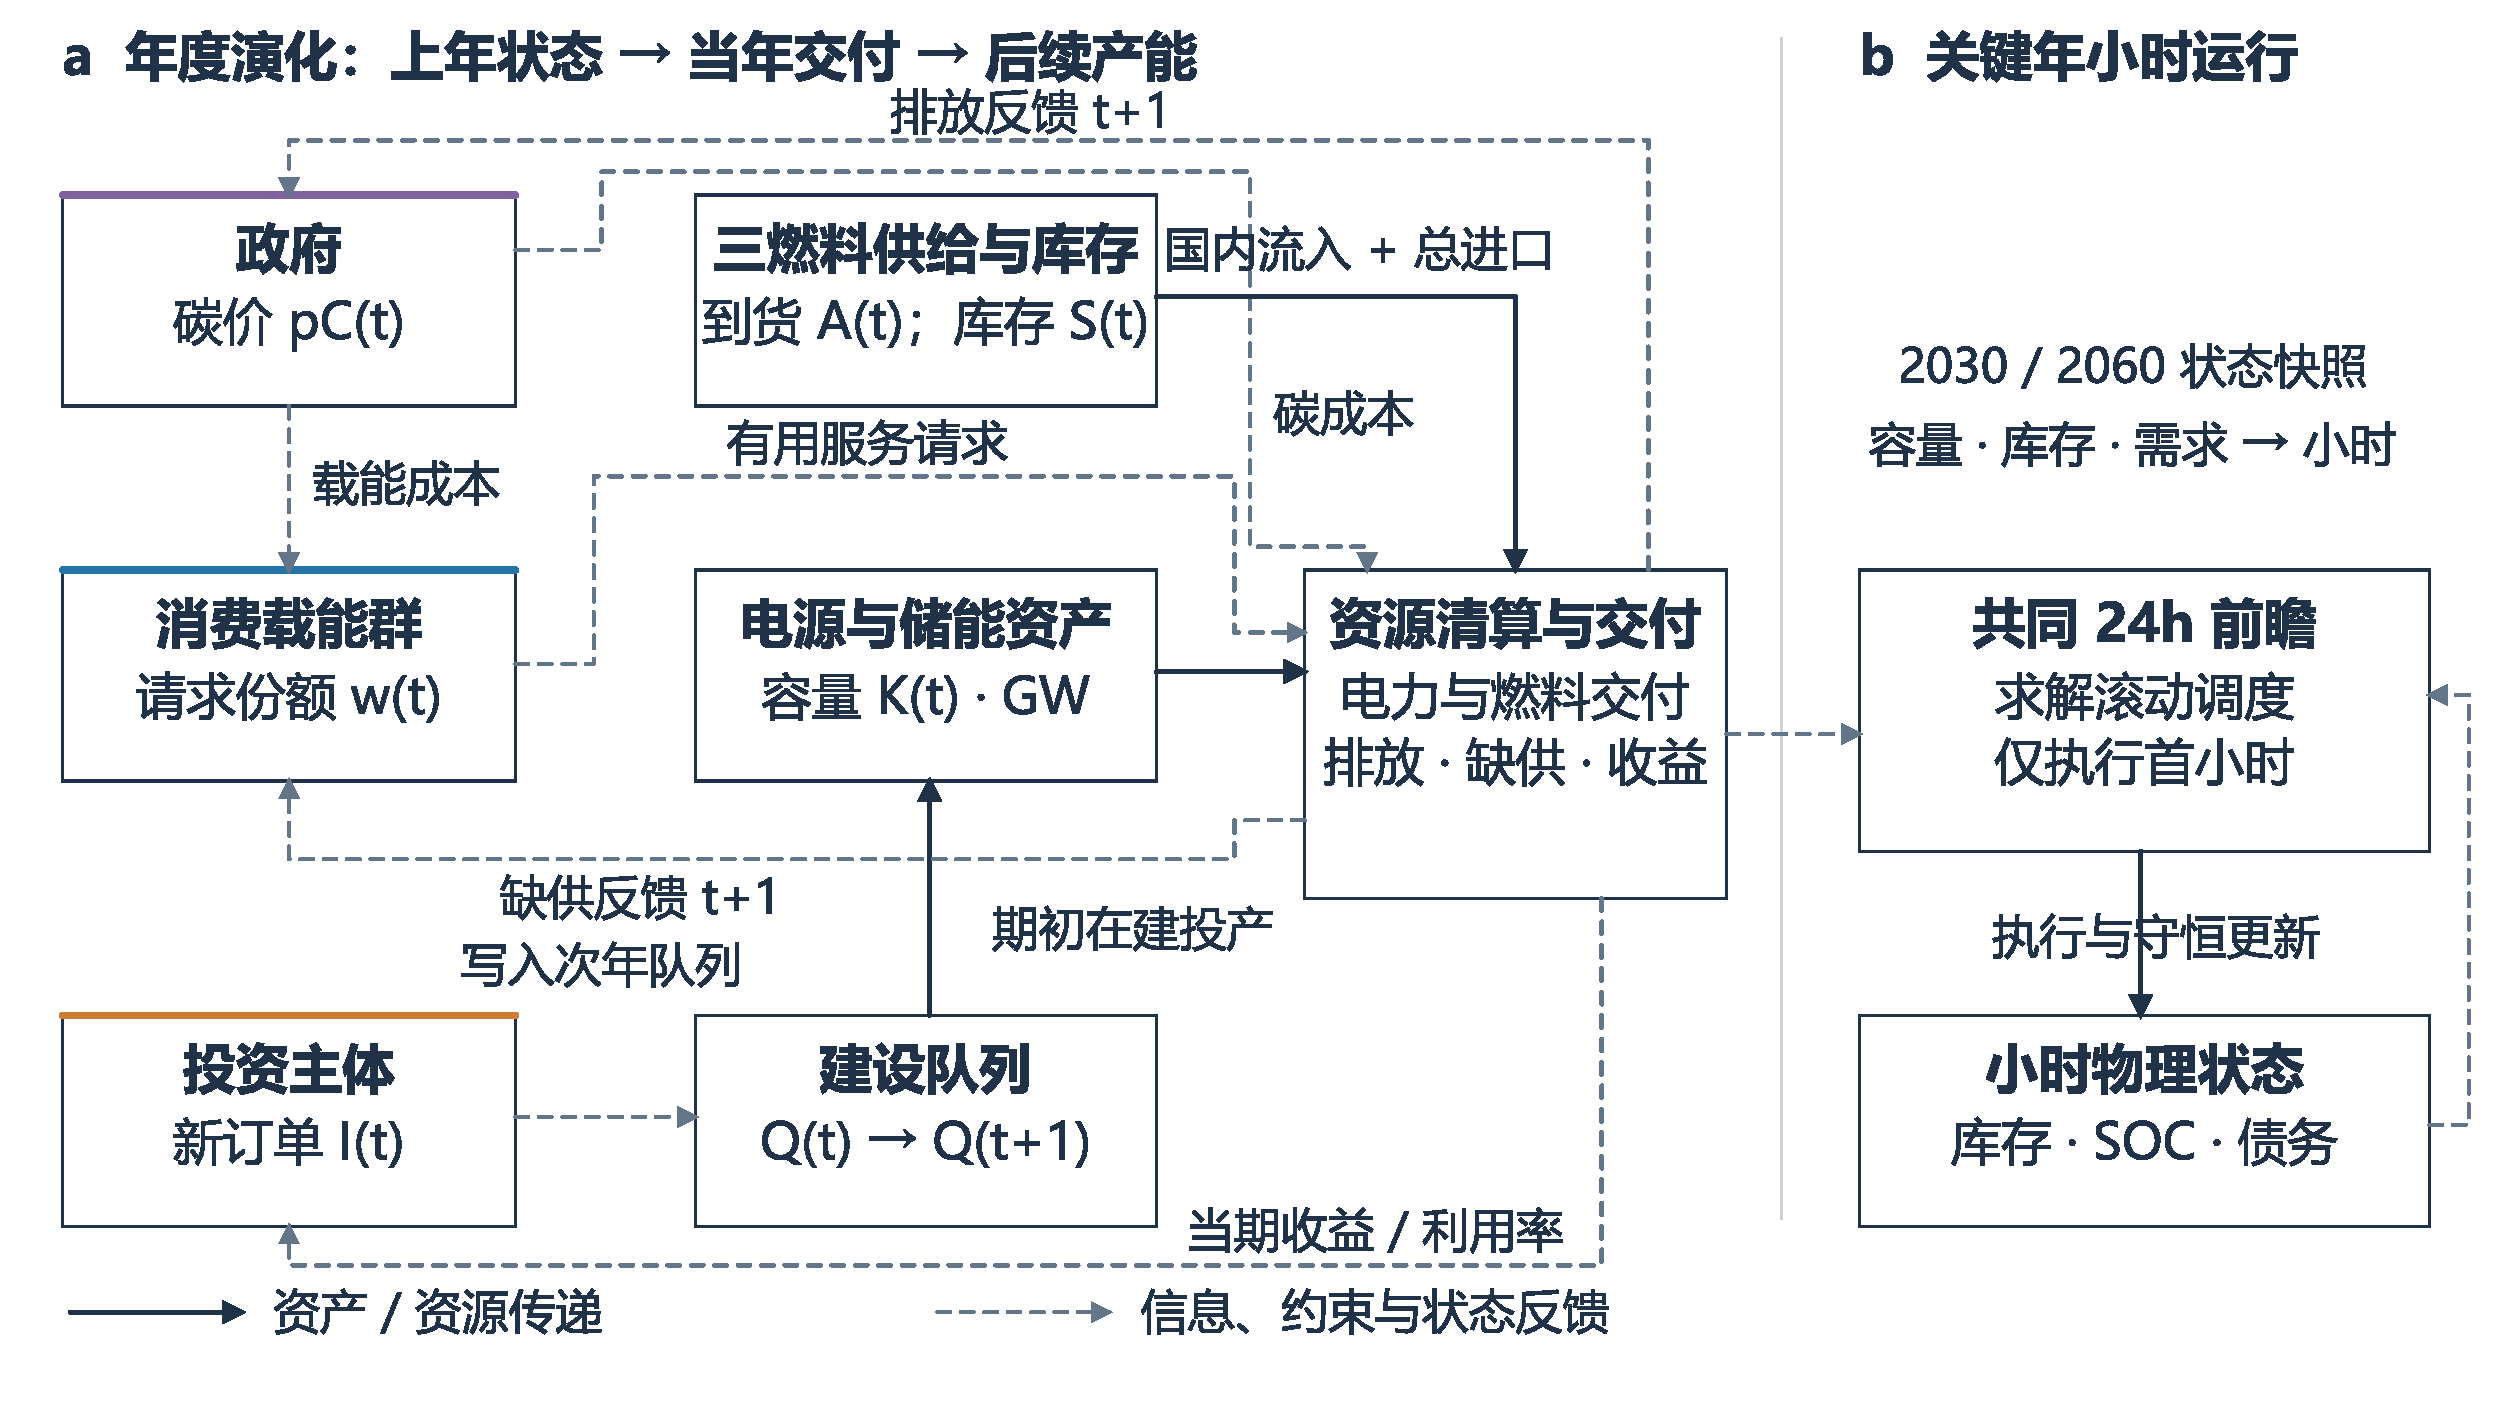
\includegraphics[width=\linewidth]{figures/fig01_system_architecture.pdf}\caption{主体决策—建设队列—资源清算—小时运行架构。实线表示物理状态或资源转移，虚线表示信息反馈；年度状态单向传入小时层。}\label{fig:fig01_system_architecture}\end{figure}


\textbf{长期转型路径能否成立，不仅取决于2060年的技术结构，还取决于此前每一年形成的供能能力及其安全约束。}因此，本文先由历史变化识别供给与结构矛盾，再用主体反事实解释长期结果，最后同时检验投资路径的逐年交付和冲击后的资源恢复。

\begin{table}[H]\centering\caption{三问的决策链与检验证据}
\begin{tabularx}{\linewidth}{p{.16\linewidth}XX}\toprule
任务 & 进入下一环节的结果 & 对应证据\\\midrule
现状评价 & 统一需求、装机、进口与库存初态 & 同版统计序列、分类口径与基年资源闭合\\
双碳推演 & 主体动作经建设队列形成关键年系统状态 & 共享历史组件、全因子机制对照与四情景指标\\
安全优化 & 投资路径筛查后，从相同初态比较运行规则与补库 & 固定方案扰动、原生反馈、强基线、能量守恒与多目标约束\\
\bottomrule\end{tabularx}\end{table}

\section{问题一：能源现状与协同潜力}
\subsection{历史总量、结构与电源演化}
历史窗口为2010—2024年，能源生产与消费采用《中国统计年鉴2025》同版次资料\cite{nbs_yearbook_2025_9_2,nbs_yearbook_2025_9_1}；电源装机和分技术发电分别使用国家统计局连续序列与Ember历史面板\cite{ember_latest_2026_10_16}，各自在原统计口径内分析。GDP为世界银行2015年不变美元序列\cite{worldbank_NY.GDP.MKTP.KD}，燃料CO$_2$为GCB经OWID整理的煤、油、气和放空分项\cite{owid_gcb_2025}。

\begin{figure}[H]\centering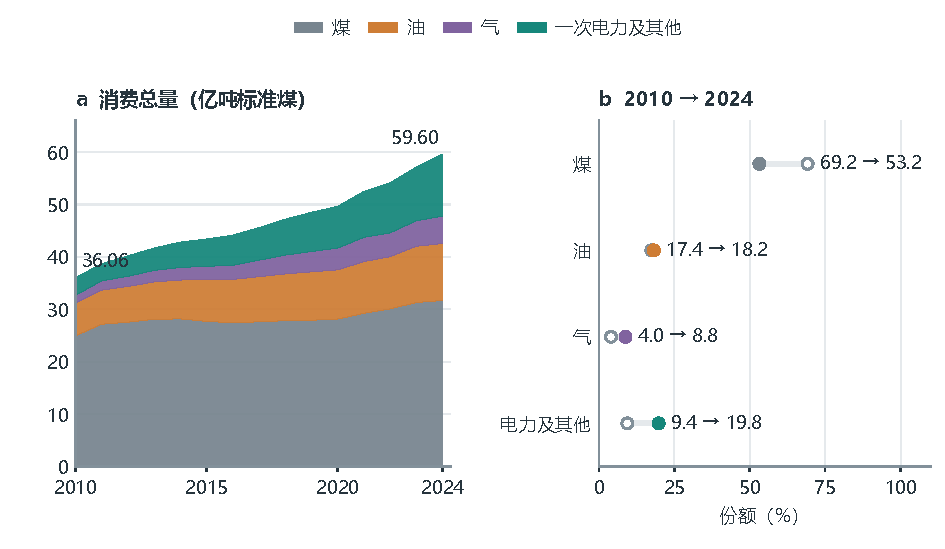
\includegraphics[width=\linewidth]{figures/fig00a_observed_consumption.pdf}\caption{同版年鉴下的一次能源消费规模与结构演变。}\label{fig:fig00a_observed_consumption}\end{figure}

\begin{figure}[H]\centering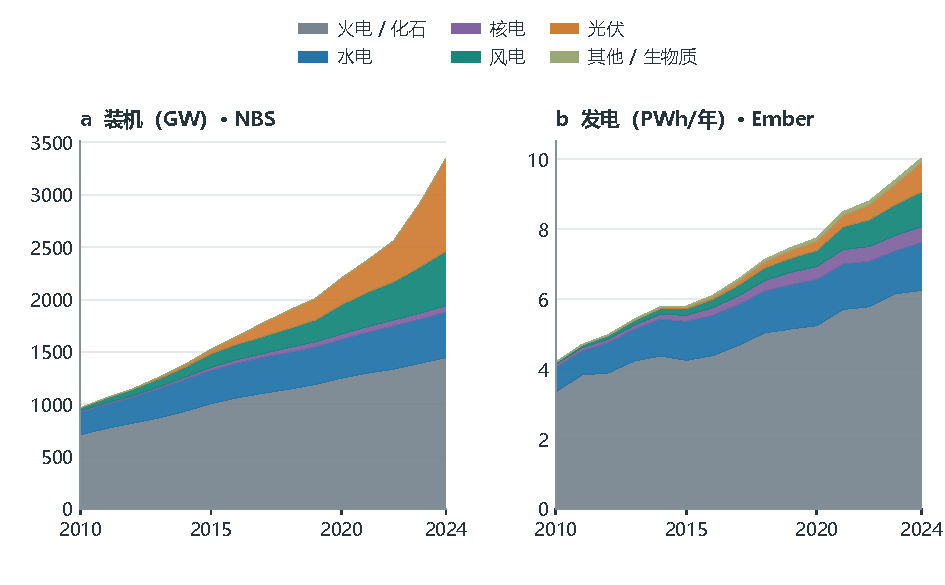
\includegraphics[width=\linewidth]{figures/fig00b_observed_power.pdf}\caption{电源装机与发电结构在各自连续统计口径内的演变。}\label{fig:fig00b_observed_power}\end{figure}

2024年一次能源消费为 5,960 Mtce，煤、油、气及“一次电力及其他能源”份额分别为53.2\%、18.2\%、8.8\%与19.8\%。历史图保留这一原始分类。Ember口径电力总需求为10069.88 TWh，国家能源局全社会用电量9852.1 TWh另按其消费端定义记录\cite{nea_electricity_2024}。电力作为二次能源，在总量核算中与发电燃料分别处理；宏观一次电力折标遵循能源平衡口径\cite{nbs_energy_method,nbs_energy_faq}。

2010—2024年一次能源消费增长65.3\%，同期实际GDP指数增长139.7\%。燃料相关CO$_2$由7.865升至11.485 Gt，增加46.0\%；2024年风光发电占比为18.3\%。能源规模增长与化石份额下降同时发生，说明结构改善需要与总量、效率和服务交付一起评价。
赛题附件1—4给出火电、水电、抽蓄、风电与核电五类电站名录，分别含633/193/31/16/17条非空记录\cite{official_station_lists}。名录的参考年份与抽样设计未声明，部分表存在重复记录，且只有抽蓄与风电提供经纬度。本文保留原始名录，用于核对给定场站规模与空间分布；全国年度总量、结构和模型初态采用上述连续统计序列，避免把名录容量直接替代全国装机。

\subsection{燃料供应、价格与区域分布}


\begin{figure}[H]\centering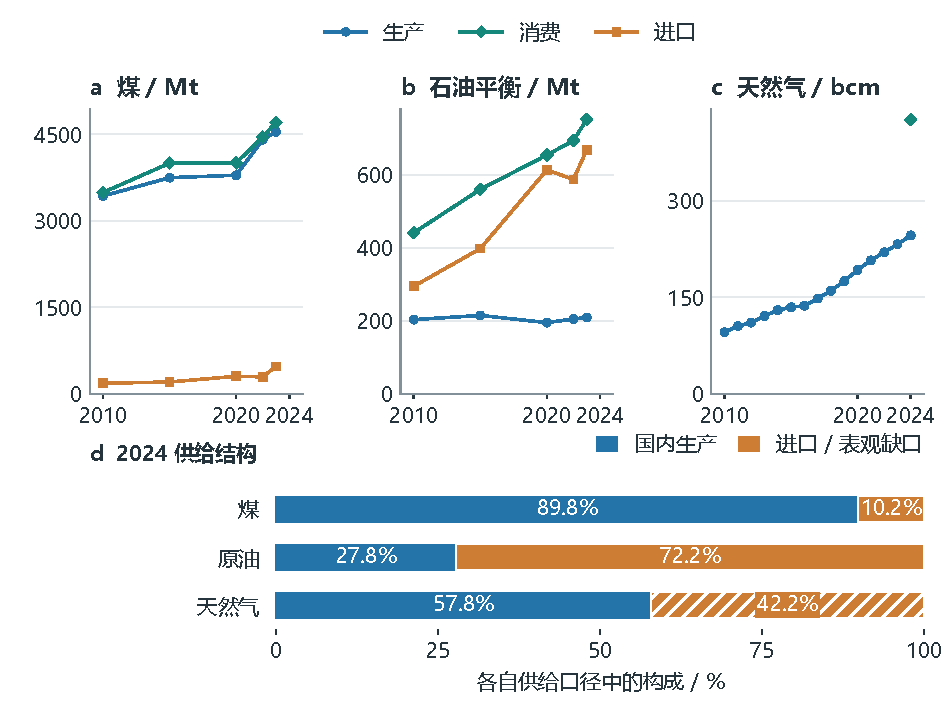
\includegraphics[width=\linewidth]{figures/fig00c_fuel_balance_exposure.pdf}\caption{三燃料历史供需与2024年供给结构。a—c保持Mt与bcm原始量纲，煤、油仅连接选定观测年，气消费仅显示2024年点。d的煤、原油比例分别以国内生产加进口为分母，气以表观消费为分母，斜纹段表示消费减生产的表观缺口。上排石油平衡含成品油贸易，下排使用原油生产与进口；气表观缺口不等同总进口。}\label{fig:fig00c_fuel_balance_exposure}\end{figure}

煤及褐煤、原油、成品油的2024年进口分别为542.70、553.42、48.23 Mt\cite{nbs_communique_2024}；天然气总进口181.7 bcm，由管道气76.0与LNG气化体积105.7 bcm构成\cite{nea_gas_development_2025}。三种燃料进口均作为独立渠道，库存、直接使用和发电领用按各自燃料守恒。

煤原料供应集中于晋陕蒙，天然气集中于西部产区，水电集中于西南。按年鉴全国总量作分母，煤前三产区约占70.30\%，天然气前三约58.37\%，水电前三约60.71\%\cite{nbs_yearbook_2025_9_19}。这种空间差异说明，能源品种的互补需要同时考虑料源、输送与灵活性。

\begin{figure}[H]\centering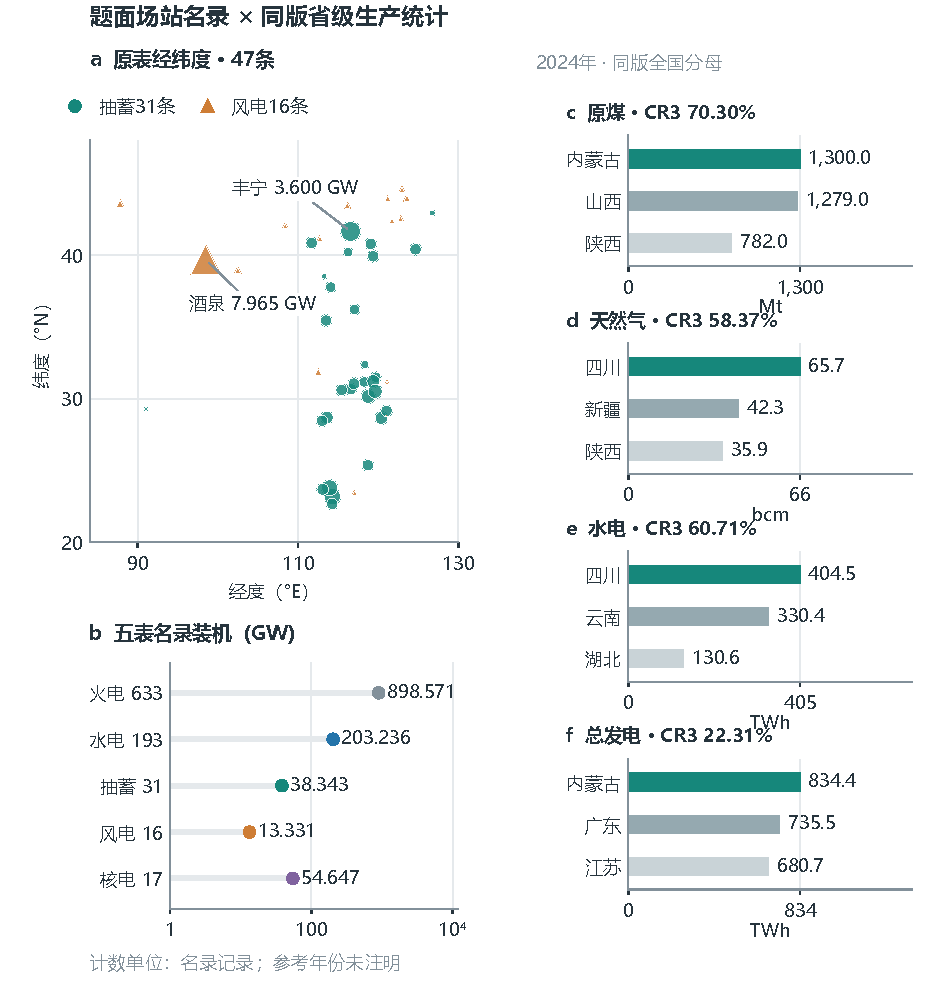
\includegraphics[width=\linewidth]{figures/fig00e_observed_regions.pdf}\caption{题面电站名录与2024年省级生产集中度。左上按附件原值绘制47条经纬度记录，点面积与装机成正比，坐标图不含行政边界；左下汇总五张表全部890条名录记录，火电、水电、核电843条未提供坐标。右侧四组沿用同版年鉴的全国分母和前三省原值。名录参考年份未注明，同名与重复记录保留，装机合计不代表2024年全国总量。}\label{fig:fig00e_observed_regions}\end{figure}

经济性以工程资本与燃料资源账分别评价。2024年12月下旬5500大卡煤767.9元/吨、LNG4413.8元/吨为流通领域价格快照\cite{nbs_prices_2024_dec_late}；长期技术资本系数采用工程参数。生物质2024年以45.99 GW和208.3 TWh成套资料建立初态\cite{nea_renewable_2024}。氢能总产量超过36.5百万吨、已建可再生电解水产能约0.125百万吨/年\cite{nea_hydrogen_2025}，纳入现状研判；本次动态模型重点评价电源、储能与三燃料交付。

现状的主要矛盾是化石燃料仍承担高比例服务、新能源发电快速增长、料源与可用出力存在空间和时间错配。协同方向对应三类资源：建设端提前形成可靠能力，运行端利用储能和服务偿还协调波动，保障端按煤油气分别维护进口渠道与库存。

\subsection{多能源发展现状的四维定量评价}
供给保障、清洁低碳、经济性与协调性分别对应不同物理量。表\ref{tab:current-four}以同口径事实识别优势与约束，再将其转为后续主体和资源规则。
\begin{table}[H]\centering\caption{2024年现状的四维定量证据与协同方向}\label{tab:current-four}
\begin{tabularx}{\linewidth}{p{.14\linewidth}p{.42\linewidth}X}\toprule
评价维度 & 定量证据 & 优势、约束与协同方向\\\midrule
供给保障 & 煤、原油进口占生产加进口分别10.2\%、72.2\%；气表观供给缺口占42.2\% & 煤具有国内供应基础，油气渠道暴露较高；按品种配置国内能力、进口与库存\\
清洁低碳 & 煤消费份额由2010年69.2\%降至53.2\%；风光发电占18.3\% & 结构改善与总量增长并存，评价排放同时检查服务交付\\
经济性 & 2024年12月下旬5500大卡煤767.9元/吨、LNG4413.8元/吨 & 分别记录燃料价格快照；工程资本、运行资源费和采购现金独立核算\\
时空协调 & 煤、气、水电前三产区占全国分别70.30\%、58.37\%、60.71\% & 料源集中与电源时序差异并存；建设工期、小时出力及资源准备共同检验\\
\bottomrule\end{tabularx}\end{table}
历史“一次电力及其他能源”19.8\%沿用年鉴原分类；前瞻模型的非化石份额另按七类电源形成。燃料吨价在各自品种和统计时点内解释，不将不同热值品种的吨价直接当作供能经济性排序。

\begin{table}[H]\centering\caption{现状证据如何进入协同模型}
\begin{tabularx}{\linewidth}{p{.14\linewidth}XX}\toprule
能源环节 & 优势与主要约束 & 模型中的实际处理\\\midrule
煤炭 & 承担主要服务，燃烧排放与料源集中并存 & 国内/进口分账，直接使用与发电竞争同一库存\\
油气 & 载能用途独立，跨境供给影响资源准备 & 两类独立进口、库存与直接服务，天然气另进入发电\\
风光 & 发电占比增长，可用出力随时段变化 & 建设订单经工期形成装机，小时可用率约束交付\\
水核生物质 & 补充稳定出力，分别受工期、来水及料源制约 & 工期队列、外生水电可用率与生物质料源预算\\
储能与移峰 & 重分配交付时点，作用受功率、能量与偿还期限约束 & 两类SOC守恒、充放功率上限与服务债务归还\\
氢能 & 可再生电解水已形成产业起点，需配套链条资料 & 现状单列；本次运行模型覆盖电源、储能与三燃料服务\\
\bottomrule\end{tabularx}\end{table}
\FloatBarrier

\section{多主体模型与历史检验}
\subsection{主体属性、行为与信息}
系统由四类有用服务载能群、七类发电投资单元、两类储能投资单元、三个燃料供给单元与政府组成。载能群按煤、油、气和电设备划分。电力市场以工程边际排序和比例燃料配给清算，形成稀缺价格与利用率反馈。

每年先从既有建设队列投产并退役，再根据历史形成的预期提出服务请求，按实际容量与料源清算。随后投资主体根据利润、利用率创新、弃电及服务缺口下单，政府根据排放误差更新下一年碳价。模型保存217个内生状态，其中180维为12类资产的15个未来投产槽。



\begin{table}[!htbp]\centering\small\caption{主体的可观察属性与实际决策}\begin{tabularx}{\textwidth}{lXX}
\toprule
主体 & 状态/接收信息 & 改变系统的动作 \\\midrule
消费载能群 & 设备份额、预期需求、相对成本、上一年缺供 & 在流量计算前改变四种载能请求份额 \\
发电/储能投资 & 装机、在建、利润、利用率、弃电与短缺 & 提出毛订单并在共同资金和建设上限内下单 \\
燃料供给 & 生产能力、进口渠道、库存与直接/发电领用 & 实际供给、库存释放与后续能力订单 \\
政府 & 实际模型排放、参考路径、既有碳价 & 改变下一期碳价，不能直接强迫净零 \\
运行清算环境 & 可用电源与同载能资源竞争 & 实现发电、直接交付、缺供、收益和稀缺信号 \\
\bottomrule
\end{tabularx}
\end{table}

\subsection{预期与载能选择}
有用服务$U_t$与电力预期由历史低维规则形成；候选为近期增量、GDP弹性和强度漂移，按每个训练起点以前的内层滚动结果选择。预期形成服务请求，装机与供给随后按物理状态实现。设$b_{f,t}$为基准预期份额，$z_{f,t-1}$为上一期缺供比例，目标份额与调整为
\begin{align}
q_{f,t}&=\operatorname{softmax}_f\{\log b_{f,t}-\beta_c\Delta c_{f,t}-\beta_z z_{f,t-1}\},\\
\tilde s_{f,t-1}&=\operatorname{norm}_f\{b_{f,t}s_{f,t-1}/b_{f,t-1}\},\quad
s_{f,t}=(1-\lambda)\tilde s_{f,t-1}+\lambda q_{f,t}.
\end{align}
其中成本为相对预期的变化，避免把固定价差逐年重复积分；$\lambda=0.5$、响应系数属于工程行为假设。先算份额，再由$D_{f,t}=U_ts_{f,t}/(\eta_f\chi)$计算直接燃料请求，$D^E_t=U_ts_{E,t}/\eta_E$计算电力请求，$\chi=29.3076/3.6$ TWh/Mtce。主动响应关闭时设$s=b_t$，保留自主趋势；独立的冻结份额诊断在流量计算前固定$s=s_{2024}$，同时移除趋势与响应。

\subsection{建设、退役与共同资本}
发电、储能和供给能力由物理存量演化：
\begin{align}
K_{j,t}&=(1-\delta_j)K_{j,t-1}+Q^{(1)}_{j,t-1},\\
Q^{(\ell)}_{j,t}&=Q^{(\ell+1)}_{j,t-1}+I_{j,t}\mathbf1\{\ell=L_j\},\qquad Q^{(16)}=0,\\
I_{j,t}&=\bar I_{j,t}\min\{1,B_t/\sum_k c_{k,t}\bar I_{k,t}\},\quad
\sum_jc_{j,t}I_{j,t}\le B_t.
\end{align}
本年末订单$I_{j,t}$经建设后供能；例如2025年下单、五年工期在2030年投产。基准工期煤/气2年、核5年、水4年、风2年、光1年、生物质2年、电池1年、抽蓄4年，燃料供应2/3/2年。历史容量差是净增，参考毛订单须加声明退役补偿。初始队列按近期吞吐推算，为后续建设时序提供工程初态。

期望订单由近期净增锚、退役补偿以及实际运行创新构成，利润响应以起点已知的市场价格与技术利用率构造参照回报，再与当年实际回报比较，避免实际市场价格和实际发电量在差分中被共同抵消。优先权仅乘在期望订单上，之后依次接受生物质料源、年度建设上限和共同资本约束，再进入建设队列。基准资本规模采用工程代理。成本下降作用于风、光、生物质和电池的资本系数，终端装机由实际订单逐期形成。



\begin{figure}[H]\centering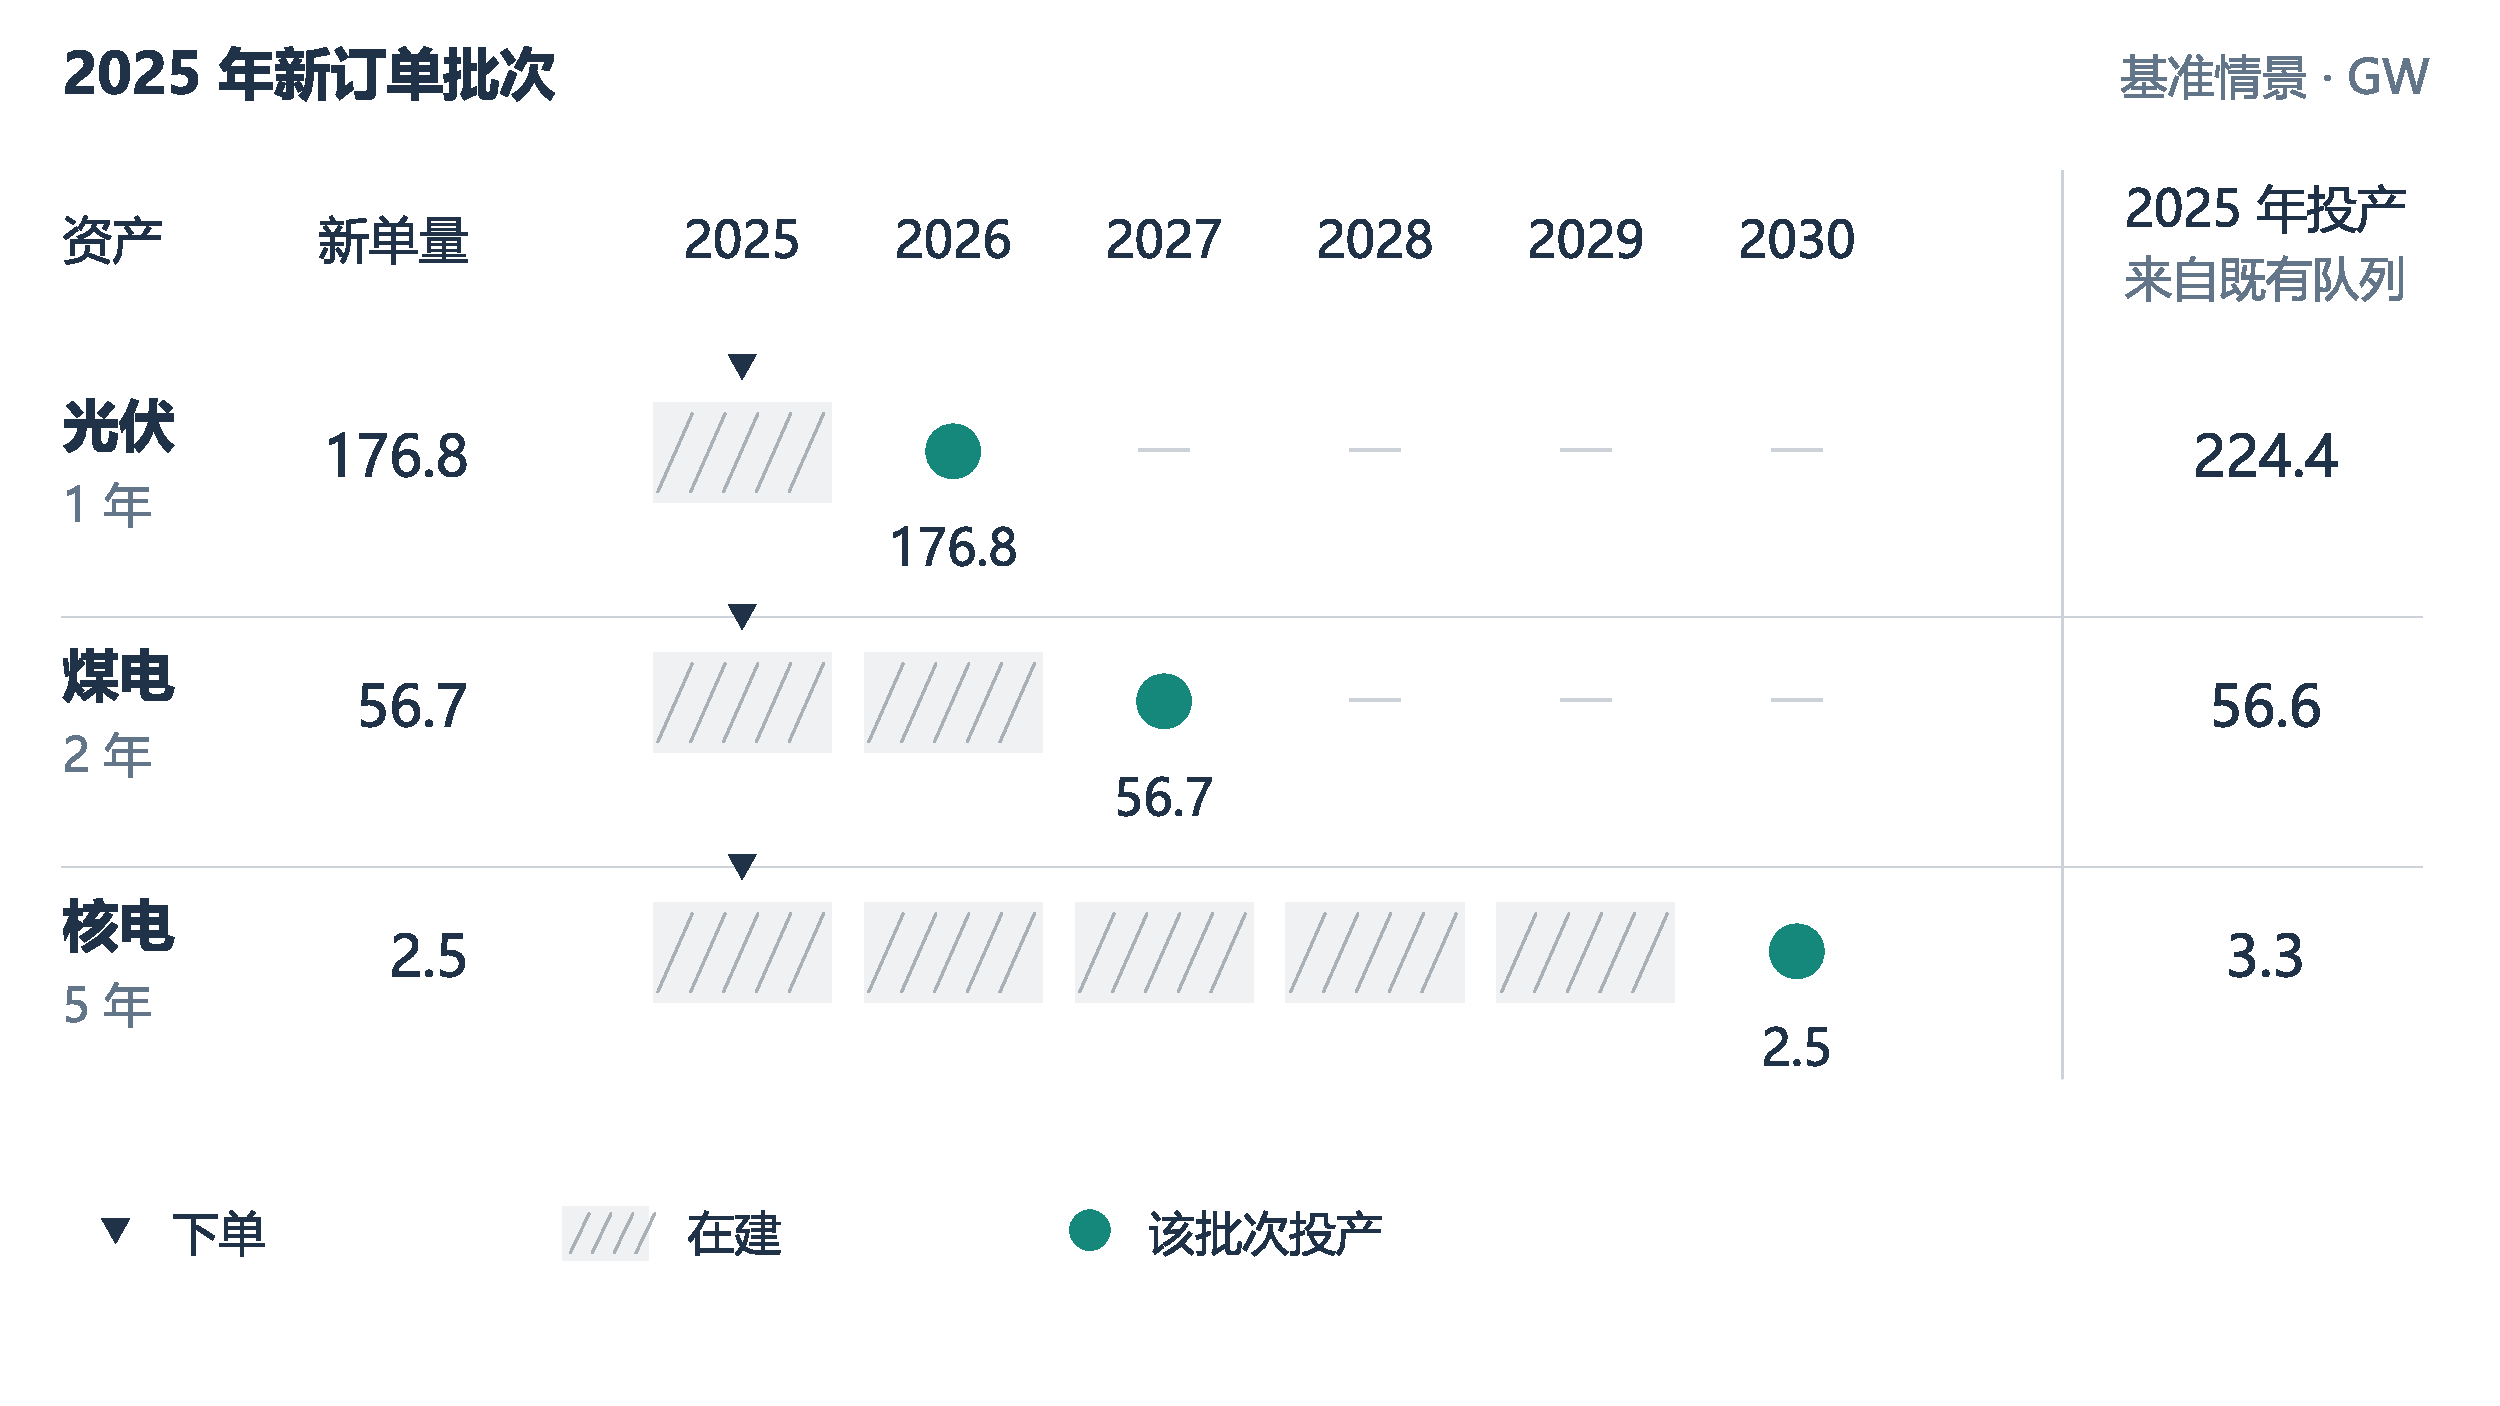
\includegraphics[width=\linewidth]{figures/fig02_queue_matrix.pdf}\caption{建设队列矩阵：2025年订单经过各技术工期后投产；同年投产的既有项目单列，避免将初始在建量归入新订单。}\label{fig:fig02_queue_matrix}\end{figure}
\subsection{可解释的投资收益响应}
投资主体的实际利润与参照利润必须由不同信息集形成。对发电技术$j$，以起点已知的利用率$u_{j,0}$、市场价$p_0$、碳价$c_0$和资本系数$C_{j,0}$构成每单位装机的参照回报，而非同时代入实际市场价与实际发电量：
\begin{align}
\pi_{j,t}&=G_{j,t}(p_t-v_j-c_t e_j)-0.08C_{j,t}K_{j,t},\\
\pi^{\rm ref}_{j,t}&=K_{j,t}\{8.76u_{j,0}(p_0-v_j-c_0e_j)-0.08C_{j,0}\},\\
\rho_{j,t}&=\frac{\pi_{j,t}-\pi^{\rm ref}_{j,t}}{\max(0.08C_{j,0}K_{j,t},1)},\qquad
m_{j,t}=\operatorname{clip}(1+0.25\rho_{j,t},0,2).
\end{align}
$G$为TWh、$p$为元/MWh，故利润以百万元计；$e_j$为年度有效燃烧映射下的排放系数。起点市场价450元/MWh、碳价100元/吨为工程初态。$m$只修正期望订单，之后仍要通过共同资本与建设上限；利用率创新、短缺及弃电另作用于订单反馈。收益响应系数0.25与8\%年资本费用为工程行为设定。该规则使当期市场价格和利用率改变后续订单，保供与排放效应由完整动态实验检验。

\subsection{独立进口渠道与基年资源闭合}
对燃料$f$，以观测国内生产$P_{f,0}$、观测消费$C_{f,0}$和独立总进口$I_{f,0}$确定国内留用比例：
\begin{equation}
r_f=(C_{f,0}-I_{f,0})/P_{f,0},\qquad 0\le r_f\le1,\qquad r_fP_{f,0}+I_{f,0}=C_{f,0}.
\end{equation}
进口渠道与国内生产能力分别演化，$r_f$作用于国内可用供应。$P_{f,0}+I_{f,0}-C_{f,0}$作为模型平衡调节项单列。进口实物量采用官方来源，折标采用工程参考：煤0.7143 tce/t，原油1.4286 tce/t，天然气1.2143 kgce/m$^3$\cite{ndrc_conversion,nbs_conversion}；成品油聚合按燃料油系数1.4286 tce/t代表。该映射同时保留煤进口和国内供应约束。

\begin{table}[H]\centering\caption{2024年三燃料的独立进口与初态闭合（Mtce）}
\begin{tabular}{lrrrr}\toprule
燃料 & 国内生产 & 总进口 & 留用比例 & 模型供应\\\midrule
煤 & 3,182.22 & 387.65 & 0.8746 & 3,170.72 \\
油 & 303.78 & 859.52 & 0.7413 & 1,084.72 \\
气 & 308.76 & 220.64 & 0.9841 & 524.48 \\
\bottomrule\end{tabular}\end{table}
\noindent{\small 表中容量、流量与留用比例按展示位数舍入，模型供应使用未舍入值计算并闭合。}\par
\subsection{燃料账与政策反馈}
煤、油、气各有独立守恒式
\begin{equation}
S_{f,t}=S_{f,t-1}+P^{\rm in}_{f,t}+M^{\rm in}_{f,t}-C^D_{f,t}-G_{f,t}/(\eta^G_f\chi).
\end{equation}
$P^{\rm in}$与$M^{\rm in}$为实际进入资源账的国内和进口流量，分别受可用上界限制；国内上界为$r_fP_{f,t}\mu^P_t$。同一燃料的直接使用与发电领用竞争当期可用供给，短缺时按请求比例配给。正常进口渠道$K^M_{f,t}$随经济规模演化，当年有效可用上界为$M^{\rm avail}_{f,t}=K^M_{f,t}\mu^M_t\eta^{\rm shock}_{f,t}$；进口倍率$\mu^M$与冲击保留率$\eta^{\rm shock}$作用于当年流量。库存补充不超过供给余量与声明补充速率。生物质发电既受容量限制，也受独立可发电料源预算限制，且该预算传入小时层。

年度排放为按历史宏观燃料消耗识别的有效映射，另加简化工业过程项。政府更新
\begin{equation}
p^C_{t+1}=\operatorname{clip}\{p^C_t+d_C+\kappa(E^N_t/E^R_t-1),\,0,\,2000\}.
\end{equation}
参考路径$E^R_t$仅影响控制误差，不直接规定真实排放。固定碳汇为800 Mt/年；模型净CO$_2$为能源与简化工业合计减该碳汇，未安装CCS。剩余移除需求$\max(E^N_t-800,0)$量化现有技术组合与目标之间的缺口。


\subsection{共享预期模块的历史检验}
以一年距2017—2023年七个起点、三年距2017—2021年五个起点检验服务预期与资产演化组件。各起点只用已有历史校准，并条件给定之后已实现GDP；动态主体、近期三年净增和持平采用同一目标。该组件沿用共享的既有预期与资产逻辑，2024年独立进口映射仅用于当前初态的前瞻试验。

\begin{figure}[H]\centering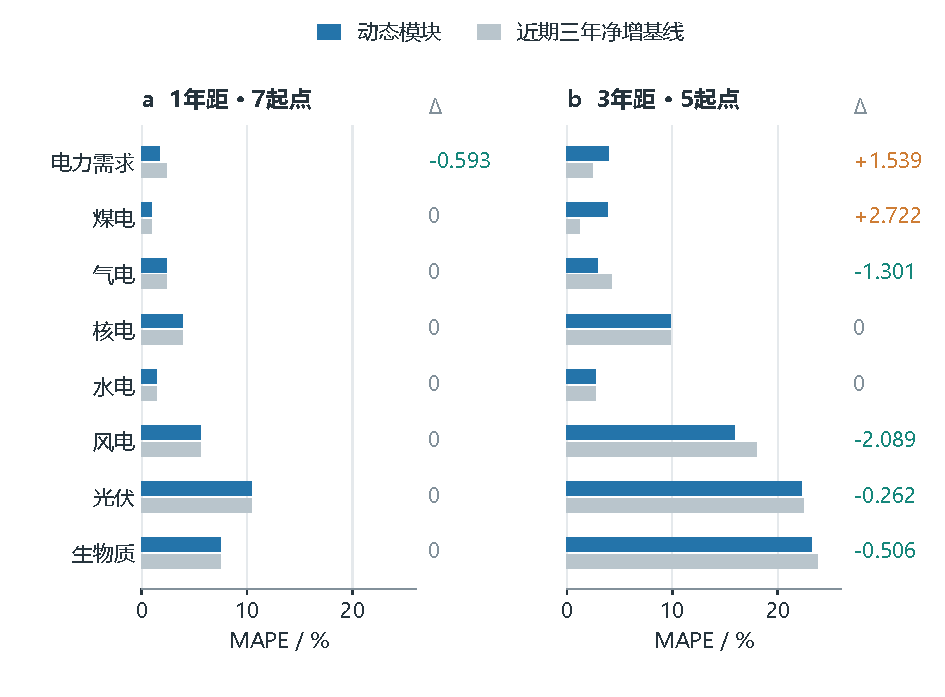
\includegraphics[width=\linewidth]{figures/fig03_validation.pdf}\caption{历史滚动验证的绝对误差与相对改进。两列同尺度横条分别为动态模块和近期三年净增基线的MAPE，右列$\Delta$为动态减基线，单位百分点；负值表示动态误差较低。全部8目标、16项比较保留；一年距7个、三年距5个起点。一年距7项容量及三年距核电、水电的两臂逐起点预测在数值精度内相等，|$\Delta$|$\le$$10^{-12}$显示0，图中其余差值保留3位小数。验证针对共享预期/资产组件，条件给定已实现GDP。}\label{fig:fig03_validation}\end{figure}

\begin{table}[H]\centering\caption{共享预期模块电力需求MAPE（\%）}
\begin{tabular}{lrrr}\toprule
预测年距 & 动态主体组件 & 近期净增 & 持平\\\midrule
1 & 1.713 & 2.306 & 5.855 \\
3 & 3.992 & 2.452 & 15.916 \\
\bottomrule\end{tabular}\end{table}

一年电力误差低于近期净增，三年则高于该基线；风光及生物质快速增长时的中期偏差更大。组件验证帮助确定条件推演的适用范围，完整资源模型另通过基年资源闭合、状态守恒和机制对照检验。
\FloatBarrier

\section{问题二：2030/2060双碳情景与主体作用}
\subsection{可比情景与目标指标}
为保持同一主体框架下的跨期可比性，本节并列展示问题二的基准推演与问题三的政策强化、供应承压和技术降本情景，后两节继续评价安全风险与投资—运行措施。四情景共享2024年初态与建设结构，GDP增速在2025—2030、2031—2040与其后分别设4.5\%、3.0\%、1.8\%。基准延续工程趋势；政策强化提高碳价漂移、资本和服务效率；供应承压在2030、2045、2060年降低进口和风光水可用出力；技术降本提高资本成本下降速率。

\begin{table}[H]\centering\caption{四情景干预参数}
\begin{tabular}{lrrrr}\toprule
情景 & 碳价漂移/元每吨年 & 年降本/\% & 资本倍率 & 年效率改善/\%\\\midrule
基准延续 & 3 & 1.5 & 1.00 & 0.0 \\
政策强化 & 9 & 2.0 & 1.15 & 0.4 \\
供应承压 & 3 & 1.5 & 1.00 & 0.0 \\
技术降本 & 3 & 4.0 & 1.00 & 0.2 \\
\bottomrule\end{tabular}\end{table}

\begin{figure}[H]\centering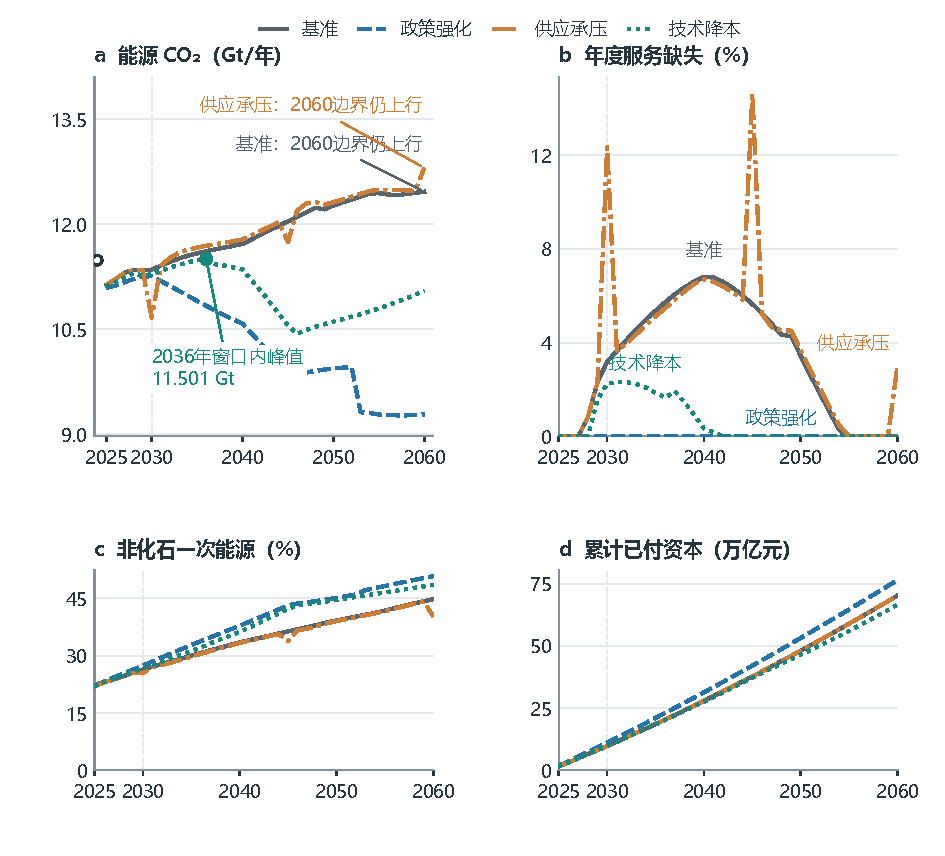
\includegraphics[width=\linewidth]{figures/figA_scenarios.pdf}\caption{终点减排与跨期交付的情景差异。排放与服务缺失为主面板，结构和资本为辅助面板；技术降本情景标注2036年窗口内峰值，末端最大值保留2060边界判定。}\label{fig:figA_scenarios}\end{figure}

\begin{table}[H]\centering\caption{2030/2060能源消费、非化石份额、排放和服务交付}
\begin{tabular}{lrrrr}\toprule
情景/年 & 一次能源/Mtce & 非化石/\% & 能源CO$_2$/Gt & 服务缺失/\%\\\midrule
基准延续/2030 & 6,716 & 26.4 & 11.351 & 3.19 \\
基准延续/2060 & 10,343 & 44.8 & 12.464 & 0.00 \\
政策强化/2030 & 6,732 & 27.4 & 11.259 & 0.00 \\
政策强化/2060 & 9,027 & 50.8 & 9.281 & 0.00 \\
供应承压/2030 & 6,071 & 25.4 & 10.664 & 12.34 \\
供应承压/2060 & 9,909 & 40.4 & 12.807 & 3.09 \\
技术降本/2030 & 6,703 & 26.7 & 11.288 & 2.25 \\
技术降本/2060 & 9,778 & 48.5 & 11.046 & 0.00 \\
\bottomrule\end{tabular}\end{table}

\begin{table}[H]\centering\caption{含2024初态的CO$_2$峰值判定}
\begin{tabular}{lrrrl}\toprule
情景 & 最大年份 & 能源/Gt & 合计/Gt & 判定\\\midrule
基准延续 & 2060 & 12.464 & 13.439 & 窗口末端，尚未确认 \\
政策强化 & 2024 & 11.485 & 12.289 & 初态为窗口最高 \\
供应承压 & 2060 & 12.807 & 13.782 & 窗口末端，尚未确认 \\
技术降本 & 2036 & 11.501 & 12.368 & 窗口内峰值 \\
\bottomrule\end{tabular}\end{table}

\begin{table}[H]\centering\caption{2060强度下降、中和率与剩余净排}
\begin{tabular}{lrrrr}\toprule
情景 & 能源强度降幅/\% & 碳强度降幅/\% & 中和率/\% & 剩余净排/Gt\\\midrule
基准延续 & 30.60 & 56.26 & 5.95 & 12.639 \\
政策强化 & 39.43 & 67.05 & 7.90 & 9.325 \\
供应承压 & 33.51 & 55.15 & 5.80 & 12.982 \\
技术降本 & 34.39 & 61.10 & 6.69 & 11.154 \\
\bottomrule\end{tabular}\end{table}

图\ref{fig:figA_scenarios}显示，技术降本的2036年峰值出现在推演窗口内部，而基准与供应承压直至2060年仍未确认达峰；这使能源结构改善与达峰判定形成不同层次的结果。能源强度以一次能源/GDP计，碳强度以能源加简化工业CO$_2$/GDP计，均相对2024年同口径初态。中和率为固定碳汇除以能源与简化工业总CO$_2$，剩余净排为总量减碳汇；固定碳汇为800 Mt/年。基准与供应承压的最大值出现在2060窗口末端，技术降本在窗口内部达到峰值，政策强化的含初态最高值出现在2024年。各结论对应给定技术和经济条件。
\subsection{多主体交互的涌现机制与条件归因}
保留自主载能趋势，仅关闭政府、消费响应或投资响应，形成四情景完整$2^3$因子实验。消费关闭时沿外生趋势形成份额；另设冻结初始份额的诊断组，考察趋势与响应共同移除的效应。政府关闭仅移除排放误差反馈，投资关闭移除收益和运行响应，所有规则仍接受同一资源约束。

\begin{figure}[H]\centering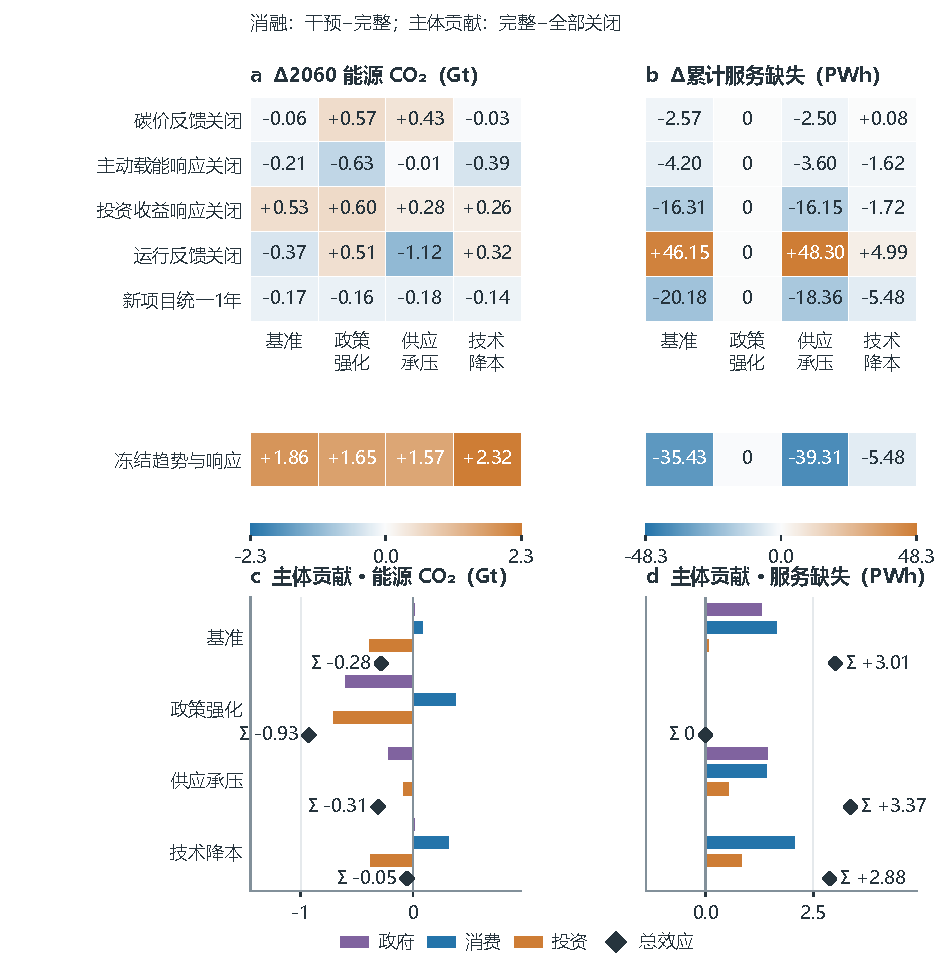
\includegraphics[width=\linewidth]{figures/figB_linked_mechanisms.pdf}\caption{主动主体反馈的减排收益与交付代价。机制反事实差值定义为干预减完整模型；条件Shapley将完整反馈减全关闭的总效应分给三主体。主动载能响应关闭保留趋势，冻结趋势另列诊断；统一一年工期只改变新订单，初始在建队列不变。}\label{fig:figB_linked_mechanisms}\end{figure}

图\ref{fig:figB_linked_mechanisms}揭示减排与交付的跨期权衡：三类主动反馈在基准下合计减少2060年能源CO$_2$ 0.283 Gt，同时增加累计未供有用服务3.011 PWh。政府价格信号、载能选择与资产订单共同作用，需沿建设队列和实际供给解释这一模型内机制结果。

投资响应的Shapley贡献为-385.330 Mt，政府与消费主动响应分别为+14.372与+87.997 Mt，后两者在这一背景下增加排放。冻结初始份额的诊断组对应消费贡献为 -2,460.877 Mt。自主趋势与主动响应对转型结果的贡献需要分开解释。



\begin{figure}[H]\centering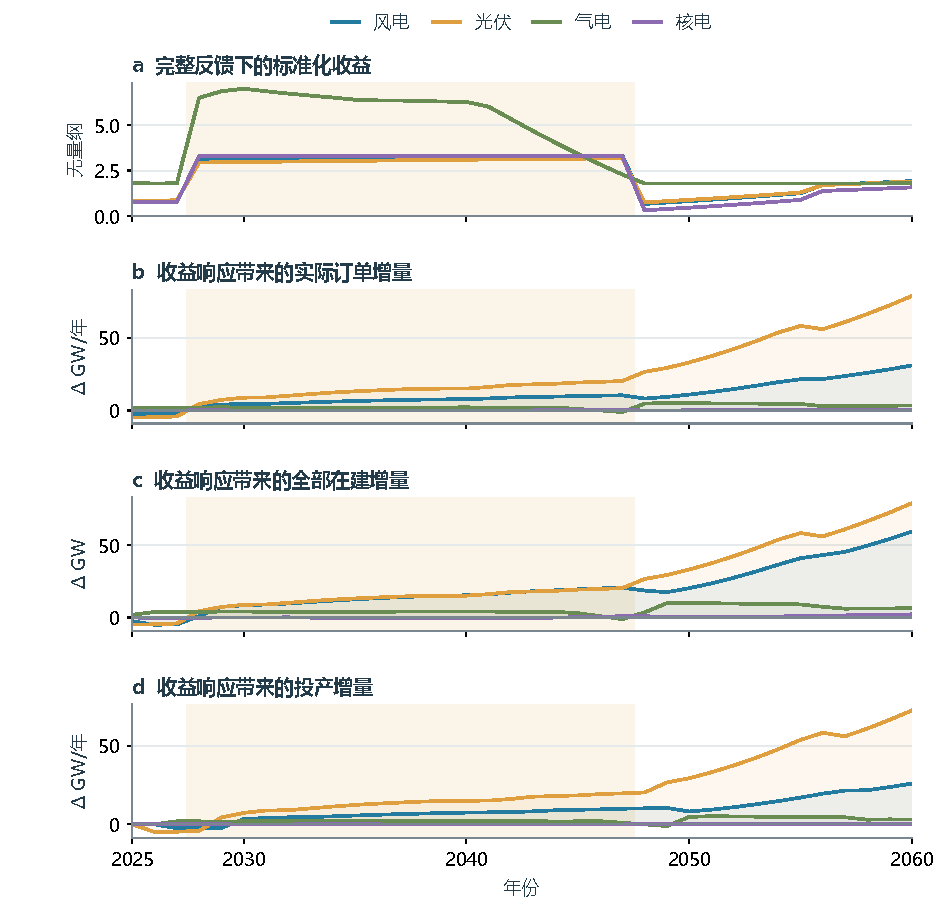
\includegraphics[width=\linewidth]{figures/figB_investment_transmission.pdf}\caption{投资收益响应的传导链。a为完整反馈的标准化收益；b—d为完整反馈减关闭收益响应的订单、全部在建及当年投产差，单位分别为GW/年、GW、GW/年。浅色区为完整反馈电价达到1200元/MWh的2028—2047年；两臂价格、四技术全部原值随表保留。}\label{fig:figB_investment_transmission}\end{figure}
\subsection{联合参数与稀缺定价敏感性}
以固定种子生成48组十维联合工程设计，改变GDP增速、技术成本、降本率、碳价、资本、建设工期、国内供应、进口和行为响应。完整执行每个设计，按排放、服务与资本共同识别敏感区间。稀缺价格另比较800、1200、1600元/MWh阶跃规则及1200元/MWh平滑规则，以检验收益反馈对定价设定的依赖。

\begin{figure}[H]\centering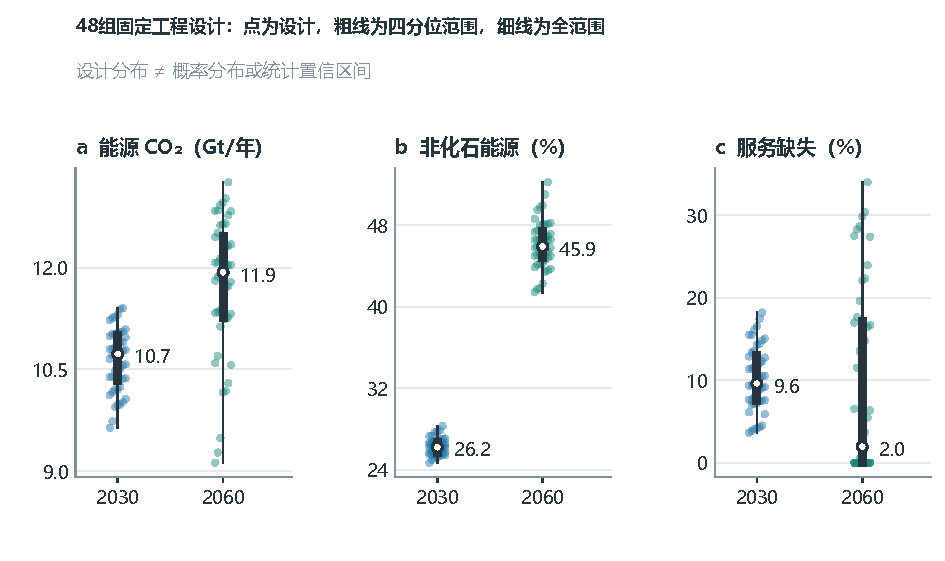
\includegraphics[width=\linewidth]{figures/fig07_joint_design.pdf}\caption{48组联合工程设计的2030与2060离散结果范围。各点为给定设计输出；中位数和极值描述设计集合，不构成概率置信区间。}\label{fig:fig07_joint_design}\end{figure}

\begin{table}[H]\centering\caption{2060年联合设计结果区间}
\begin{tabular}{lrrr}\toprule
指标 & 最小 & 中位 & 最大\\\midrule
能源CO$_2$/Gt & 9.12 & 11.93 & 13.26 \\
非化石/\% & 41.45 & 45.94 & 52.24 \\
服务缺失/\% & 0.00 & 1.95 & 33.98 \\
累计付资/万亿元 & 53.04 & 68.67 & 85.31 \\
\bottomrule\end{tabular}\end{table}

\begin{table}[H]\centering\caption{基准稀缺定价敏感性}
\begin{tabular}{lrr}\toprule
价格规则 & 2060能源CO$_2$/Gt & 累计服务缺失/PWh\\\midrule
阶跃800 & 12.664 & 19.608 \\
阶跃1200 & 12.464 & 35.427 \\
阶跃1600 & 12.411 & 46.642 \\
平滑1200 & 12.648 & 20.687 \\
\bottomrule\end{tabular}\end{table}

\begin{figure}[H]\centering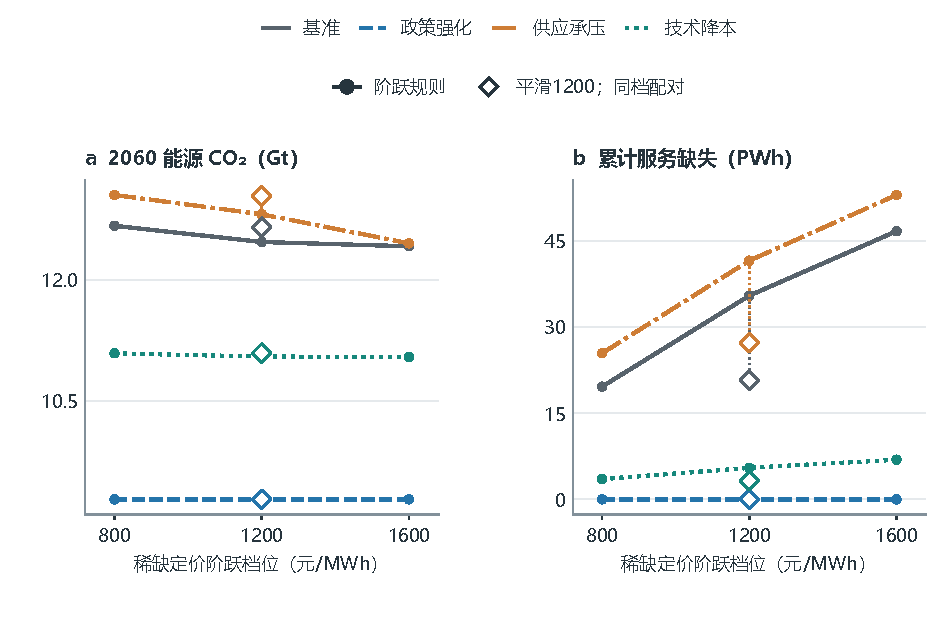
\includegraphics[width=\linewidth]{figures/fig14_price_response.pdf}\caption{稀缺定价的两类干预。阶跃800、1200、1600按数值档位比较，平滑1200以独立标记与阶跃1200配对；函数形状不当作价格数轴延伸。}\label{fig:fig14_price_response}\end{figure}

基准条件下，将稀缺定价阶跃档位由800调整至1200元/MWh，2060年能源CO$_2$由12.664 Gt降至12.464 Gt，而累计未满足服务由19.608 PWh增至35.427 PWh。较强稀缺信号改变利润、订单及后续供给路径，终点排放与跨期交付因此出现不同方向的变化。这是给定工程价格规则下的条件比较，不能直接外推为现实电价变化的数量效应。进口参考折标的敏感性同时保持基年物理留用比例约束；原低档试算因留用比例超过1判为输入不可行，修订后的低档与高档按新协议单独保存。联合工程设计用于比较条件变化。

\section{问题三：能源安全与投资—运行优化}
\subsection{可靠性约束下的投资路径}
沿用前节可比情景，安全评价采用服务交付、能源及料源约束、工程资本、重复冲击后库存恢复四个维度。年度路径要求2030—2060每年电力、各直接燃料和有用服务缺失均不超过1\%；投资决策包括三期预算、六组订单优先级及碳价漂移，共10维。每个候选从同一2024初态重新演化，投资支出通过资产建设队列，在相应投产年份转化为可用供给能力。
\begin{align}
\min_{x\in\mathcal X}\;&\big(C_{\rm cap}(x),E^{\rm net}_{2060}(x),R(x)\big),\\
C_{\rm cap}(x)&=\sum_{t=2025}^{2060}\sum_j\frac{c_{j,t}I_{j,t}(x)}{(1.04)^{t-2024}},\\
R(x)&=\max_{t\ge2030}\{r^E_t,r^D_{{\rm coal},t},r^D_{{\rm oil},t},r^D_{{\rm gas},t},r^U_t\}\le0.01.
\end{align}

\begin{figure}[H]\centering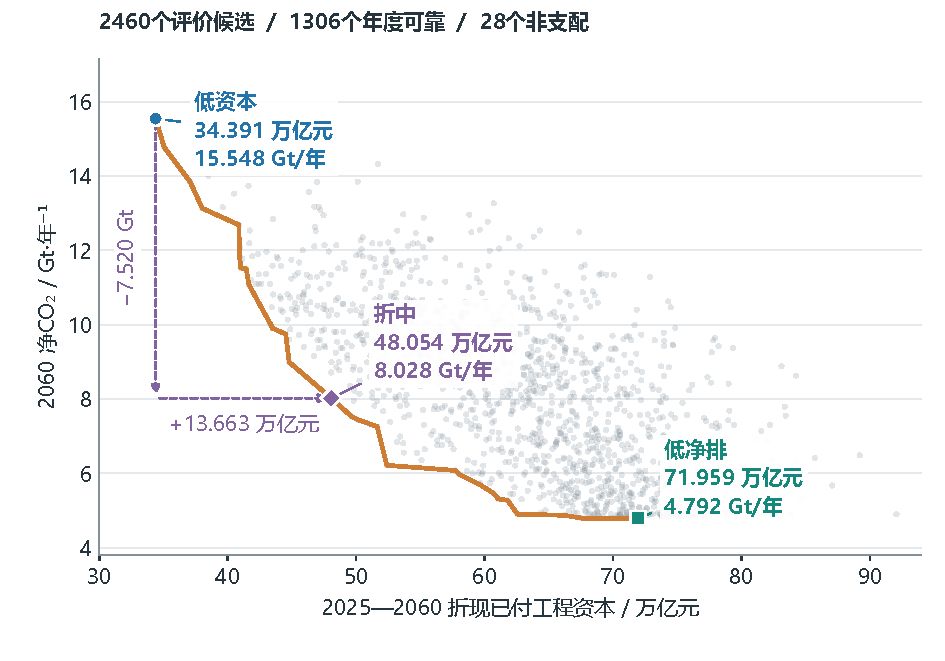
\includegraphics[width=\linewidth]{figures/figC_capital_frontier.pdf}\caption{年度可靠性约束下的资本—净排取舍。2460个评价候选中1306个年度可靠，橙线连接其中28个非支配点，三个代表点直接标注资本与净排坐标。紫色虚线箭头分解折中相对低资本的差值：资本增加13.663万亿元，2060年净排减少7.520 Gt。资本为2025—2060已付工程资本按4\%折现至2024年；技术域独立推导下界为0.175 Gt，五次固定预算搜索均未收敛。}\label{fig:figC_capital_frontier}\end{figure}

\begin{table}[H]\centering\caption{可靠性、工程资本与2060净排放的取舍}
\begin{tabular}{lrrl}\toprule
候选 & 折现资本/万亿元 & 净排/Gt & 年度可靠\\\midrule
基准参照 & 35.303 & 12.639 & 否 \\
8 Gt目标候选 & 49.643 & 7.533 & 是 \\
12 Gt目标候选 & 40.929 & 11.843 & 是 \\
最低观察净排 & 71.959 & 4.792 & 是 \\
最低观察可靠资本 & 34.391 & 15.548 & 是 \\
资本—净排折中 & 48.054 & 8.028 & 是 \\
\bottomrule\end{tabular}\end{table}

图\ref{fig:figC_capital_frontier}共评价2460个不同控制向量，1306个满足年度可靠性，形成28点已评价前沿。折中候选以48.054万亿元折现工程资本形成8.028 Gt净排路径；相对最低观察可靠资本，多投入13.663万亿元，净排减少7.520 Gt。五项固定预算搜索均达到迭代上限而未收敛，所得候选用于明确可执行的资金与技术组合。

模型2060年简化工业排放约975.346 Mt、碳汇800 Mt，能源排放非负，因而当前技术域净排下界为175.346 Mt。零净排需要扩展工业减排或新增移除能力；4 Gt目标的固定搜索尚未找到可靠候选，8和12 Gt目标已有可行路径。
\clearpage
\subsection{增量资本如何转化为不同供给组合}
折中方案多投入13.663万亿元，核水生物质、风光及燃料供应分别增加8.249、7.608、2.349万亿元，煤气发电与储能分别减少4.351、0.192万亿元。阶段长6、10、20年，年均折现增量为0.413、0.208、0.455万亿元，后期总额同时包含时间窗口长度与年均投入变化。

2060年煤气发电由14.563降至4.513 PWh，储能由179.488降至157.269 GW。三条路径均年度达标，同一连续冲击后段未供电却为0、56.870、0 TWh；这组完整组合比较说明，年度可行路径仍需冲击筛查。

\begin{figure}[H]\centering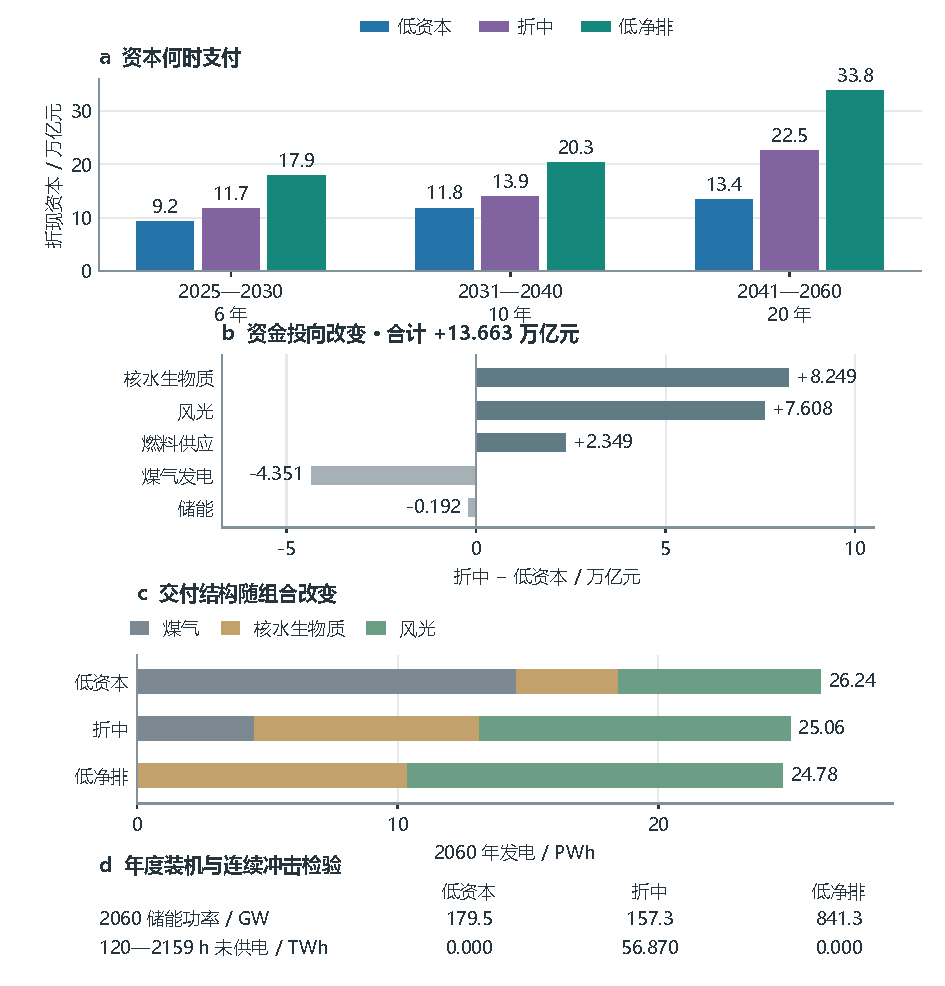
\includegraphics[width=\linewidth]{figures/figC2_investment_translation.pdf}\caption{资金投向、供给结构与冲击暴露的组合比较。a按6/10/20年分段汇总折现资本；b为折中减低资本的资金差，五组合计13.663万亿元；c为2060绝对发电量；d分列同年储能功率与连续事件h120—2159缺供。资金技术分解为完整路径的描述性分解。}\label{fig:figC2_investment_translation}\end{figure}

\clearpage
\subsection{连续小时检验与滚动协同}

\begin{figure}[H]\centering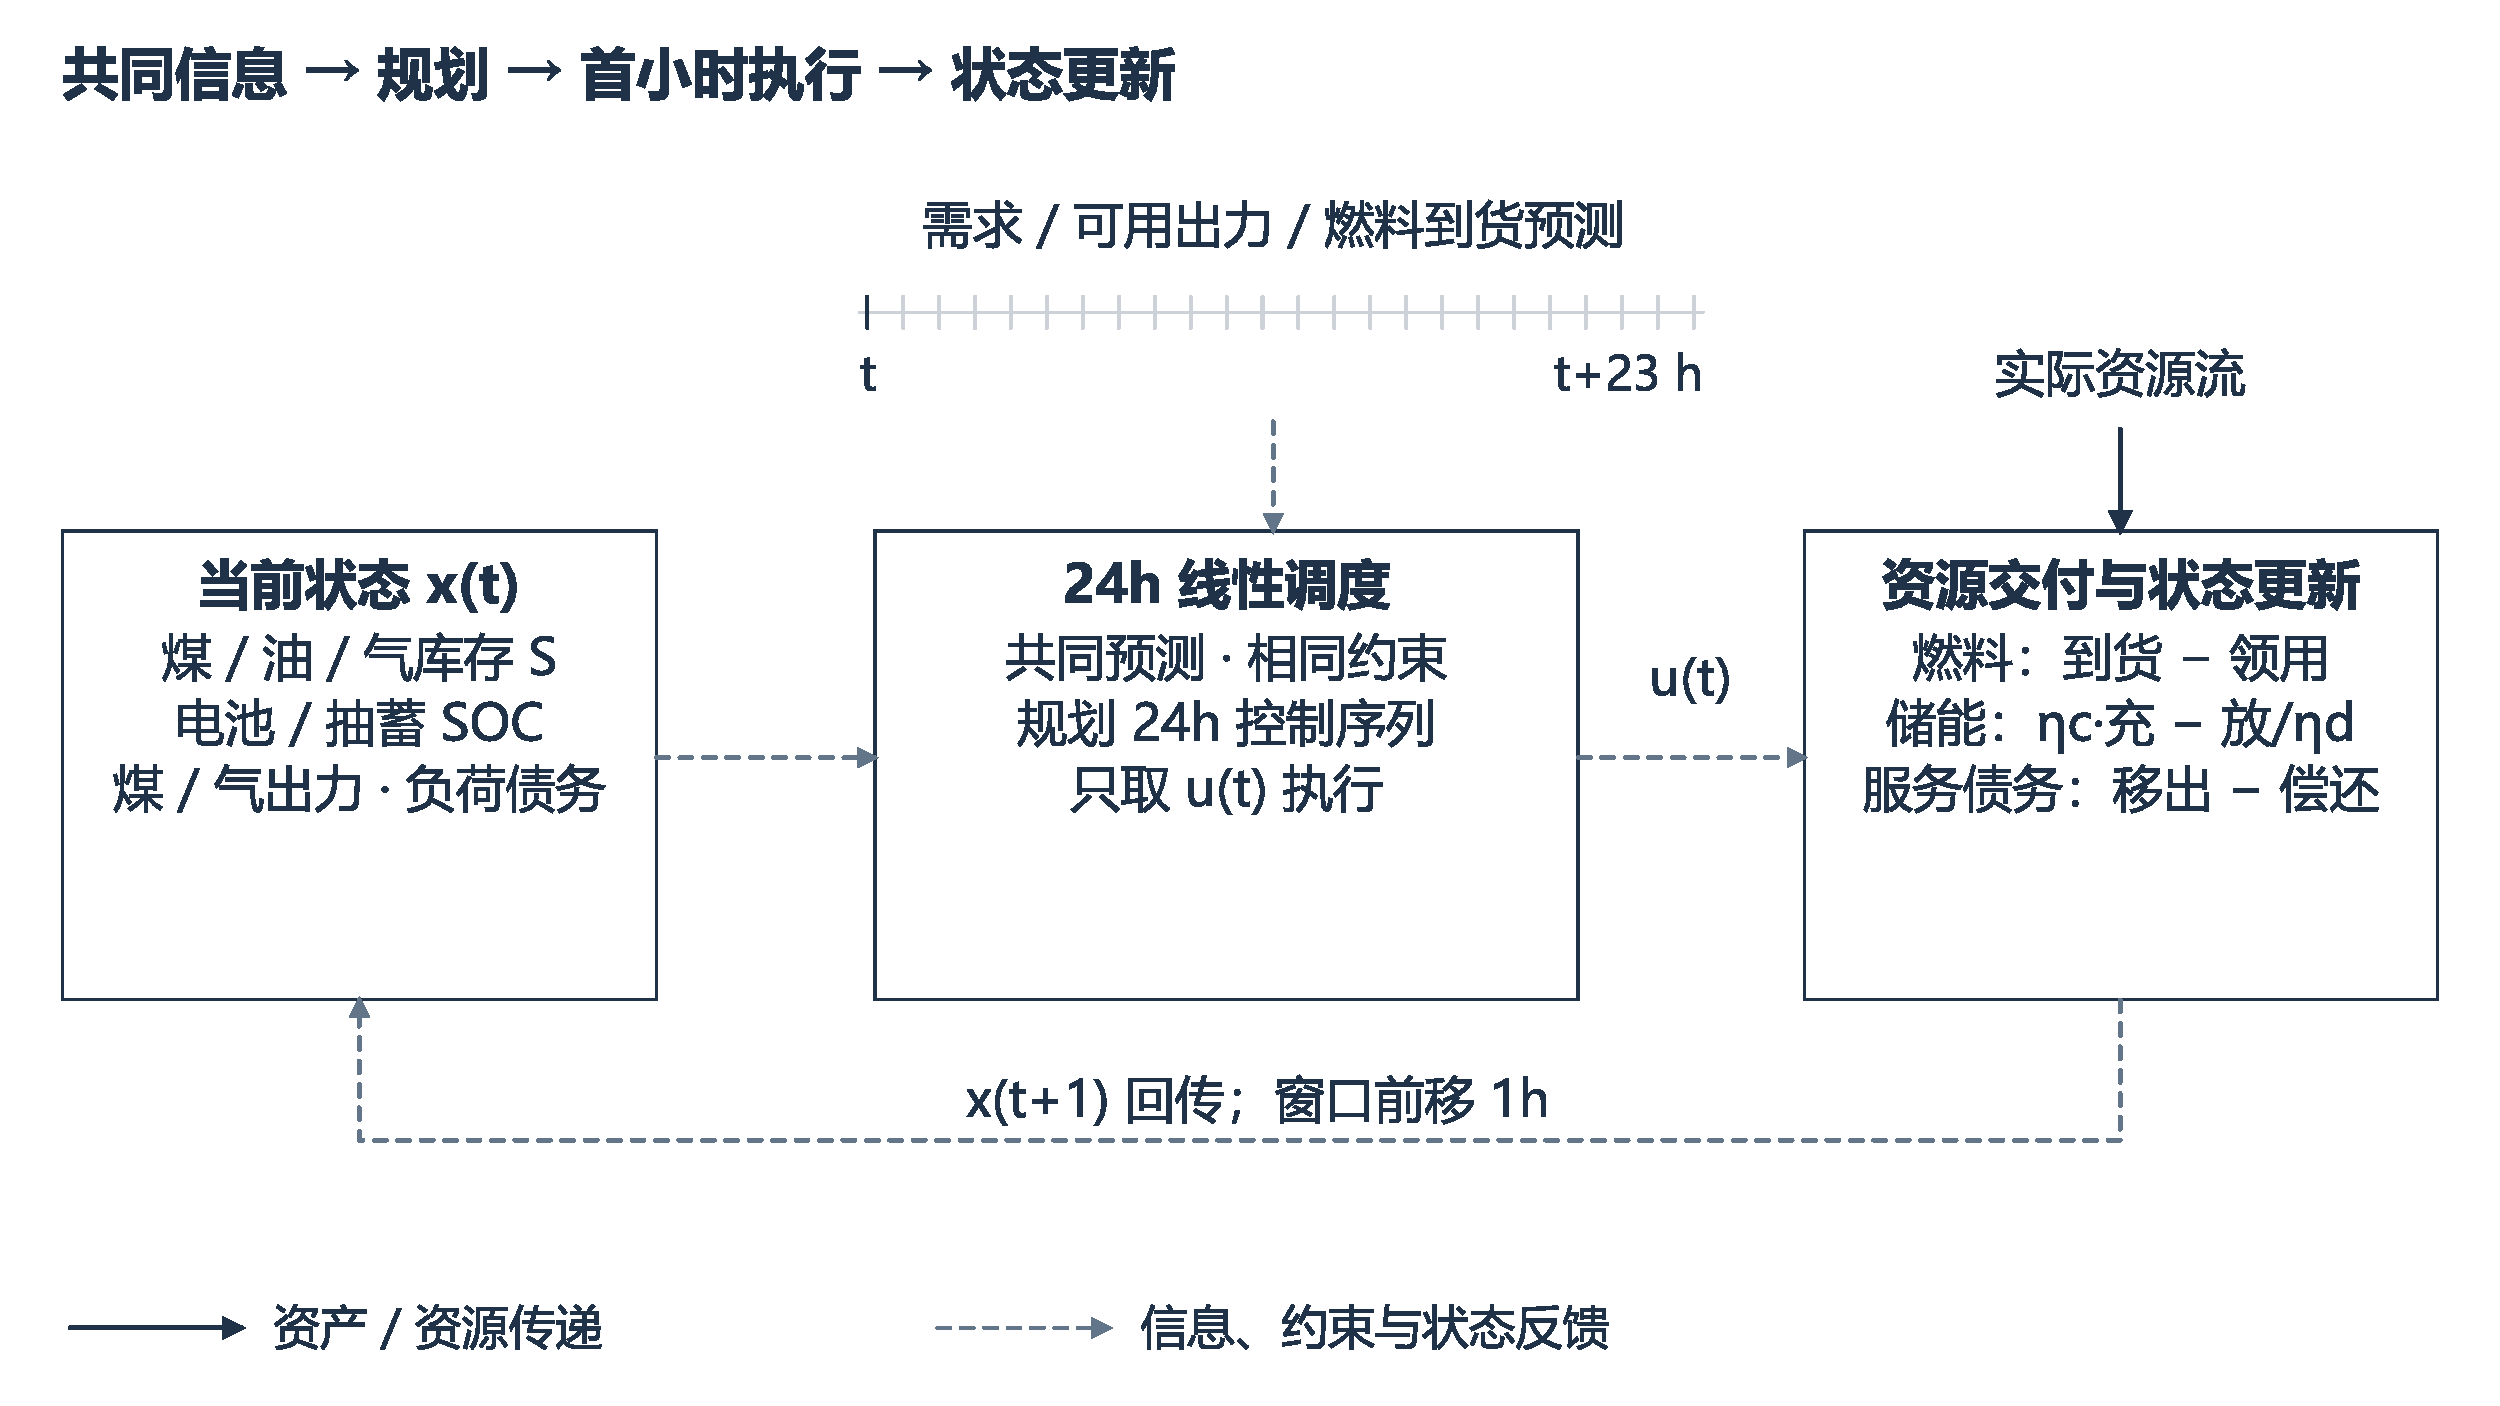
\includegraphics[width=\linewidth]{figures/fig03_rolling_control.pdf}\caption{滚动协调以当前状态和共同前瞻求解，仅执行首小时行动，再以更新库存、SOC与负荷债务进入下一小时。}\label{fig:fig03_rolling_control}\end{figure}

将三类代表投资路径的2030/2060年模拟装机、需求、料源流量、年末库存与进口渠道传入小时层。本节协调与指定非化石局部储能规则共享24小时完美前瞻，每步求解线性规划，仅执行首小时\cite{mathworks_linprog}。协调联合决定储能与资源分配；该局部规则先按需求减非化石可用出力的净负荷预期确定本地储能动作，再由同一调度器分配其余资源。燃料、SOC、热机爬坡记忆与负荷债务连续继承。
\begin{align}
S_{f,h+1}&=S_{f,h}+A_{f,h}-d_{f,h}-\mathbf1_{\{f\in\{\text{煤},\text{气}\}\}}g_{f,h}/(\eta_f\xi),\quad S_{f,h+1}\ge0,\\
E_{b,h+1}&=E_{b,h}+\eta_b^cp^c_{b,h}-p^d_{b,h}/\eta_b^d,\quad0\le E_{b,h}\le\bar E_b,\\
Z_{h+1}&=Z_h+u_h-v_h,\quad Z_{24k}=0,\quad Z_H=0,\\
g_{f,h}-g_{f,h-1}&\le R_f,\qquad0\le g_{j,h}\le\bar g_{j,h},\\
g_{f,h-1}-g_{f,h}&\le\max\{R_f,(\bar g_{f,h-1}-\bar g_{f,h})_+\},\quad f\in\{\text{煤},\text{气}\}.
\end{align}
$\xi=8141$ GWh/Mtce，煤油气化石燃烧采用IPCC默认系数\cite{ipcc}；油仅供直接服务。煤、油分别以烟煤和原油因子作聚合代表，生物源CO$_2$与生命周期排放另属其他核算范围。上爬坡受常规速率限制，下爬坡允许可用出力下降引起的受迫停机。初末库存与SOC均按同一残值计价，资源费用、合同采购现金、失供惩罚和碳价转移分别记录，生物质料源上限由年度预算传入。

每组连续运行2160小时：预运行$[0,120)$，两次冲击$[120,600)$、$[1200,1680)$，中间及末段恢复。冲击期间煤、油、气进口保留50\%、5\%、5\%，风、光、水可用出力保留25\%、55\%、70\%，电需求增加8\%。每次恢复48小时后才可有付费合同到货；合同流率不超过正常进口渠道容量50\%，每次量不超过初始库存50\%，溢价50\%。

\begin{figure}[H]\centering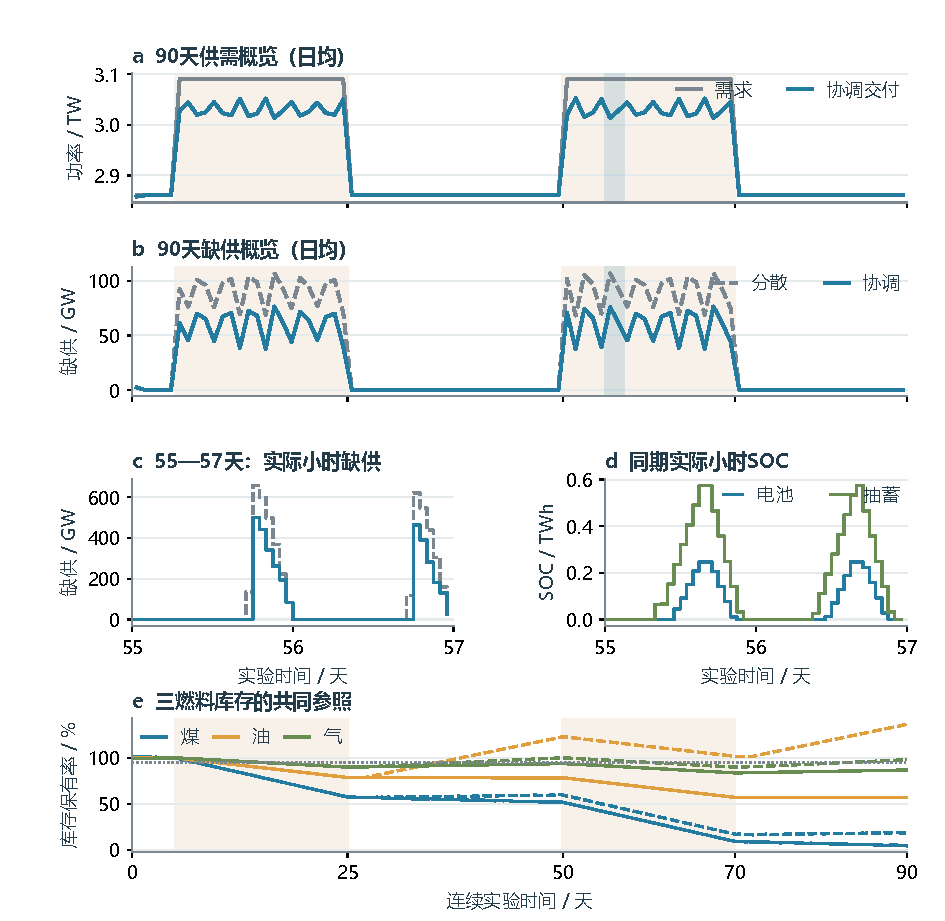
\includegraphics[width=\linewidth]{figures/figD_continuous_shocks.pdf}\caption{连续90天的运行协调与资源准备。a—b为日均功率，c—d放大55—57天实际小时缺供与SOC；浅色为两次冲击。e按三燃料各自h119库存统一归一，实线为继承供应、虚线为付费补库；95\%仅为首次事件前库存参照，不表示每次事件前归一的连续24小时联合恢复门。}\label{fig:figD_continuous_shocks}\end{figure}

\begin{table}[H]\centering\caption{继承供应下的服务交付比较}
\begin{tabular}{lrrr}\toprule
路径/年 & 预运行协调/GWh & 后续协调/TWh & 后续分散/TWh\\\midrule
最低观察可靠资本/2030 & 200.567 & 0.000 & 0.000 \\
最低观察可靠资本/2060 & 463.006 & 0.000 & 0.000 \\
资本—净排折中/2030 & 231.620 & 0.000 & 0.000 \\
资本—净排折中/2060 & 58.415 & 56.870 & 86.505 \\
最低观察净排/2030 & 109.971 & 0.000 & 0.000 \\
最低观察净排/2060 & 0.000 & 0.000 & 0.000 \\
\bottomrule\end{tabular}\end{table}

图\ref{fig:figD_continuous_shocks}中，折中2060年协调未供电为56.870 TWh，分散为86.505 TWh，减少29.635 TWh（34.3\%）；其余五类快照的预运行后电力缺失均为零。合同补库保持相同电力缺失，说明本组的新增燃料与发电可用能力约束承担不同作用。关闭煤进口渠道的同初态对照未供电上升至462.801 TWh，直接显示跨境料源对安全结果的影响。

\begin{table}[H]\centering\caption{折中2060路径的运行费用、排放与合同现金}
\begin{tabular}{lrrrr}\toprule
策略 & 后段缺供/TWh & 资源费/万亿元 & CO$_2$/Gt & 合同现金/万亿元\\\midrule
继承供应/协调 & 56.870 & 2.852 & 2.909 & 0.000 \\
继承供应/分散 & 86.505 & 2.845 & 2.894 & 0.000 \\
合同补库/协调 & 56.870 & 3.137 & 2.909 & 0.854 \\
合同补库/分散 & 86.505 & 3.130 & 2.894 & 0.854 \\
\bottomrule\end{tabular}\end{table}

费用与排放覆盖完整2160小时，缺供列为预运行后的累计值。资源费计燃料、非化石运行、储能、移峰、库存占用与合同溢价；合同全额采购现金单列。协调比同供应分散策略增加14.412 Mt排放与71.54亿元工程资源费，换取29.635 TWh交付改善。合同补库维持相同交付与排放，增加0.854万亿元采购现金并提高末期库存，反映保障储备的实际代价。
\subsection{区分服务恢复与资源恢复}
服务恢复按冲击后第一个连续24小时窗口的累计电力及各直接燃料缺供率不超过1\%判定；联合库存恢复还要求该窗口每小时三种燃料均达到各自事件前库存95\%。同一观察窗内未达到时保留未恢复状态。

\begin{figure}[H]\centering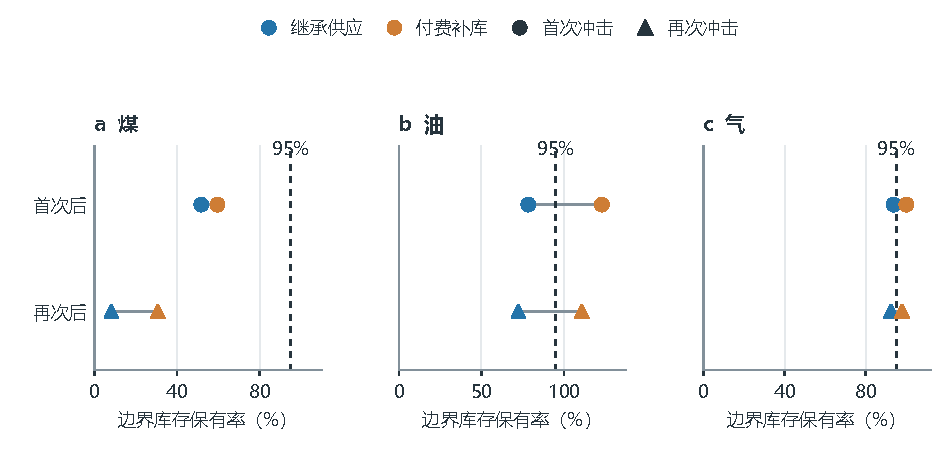
\includegraphics[width=\linewidth]{figures/fig15_service_and_stocks.pdf}\caption{服务恢复与资源准备的分离。颜色表示供给方式，形状表示冲击次数，配对线连接h1200与h2160观察边界的库存。分母为各策略各次事件前库存，95\%为对应恢复参照；与连续轨迹的首次事件前固定分母不同。}\label{fig:fig15_service_and_stocks}\end{figure}

54次事件评估中，52次首个服务窗口满足门槛，2次服务在观察窗内未恢复；全部联合库存恢复仍未达到。合同为煤提供了正到货并改善期末煤库存，三燃料的改善程度不同。零煤渠道对照则保持煤补库为零。由此，储能协调、燃料补库和建设能力应分别针对运行时序、料源和供能上限配置，服务重新达标后仍需持续追踪资源储备。

\subsection{固定投资路径的联合扰动复验}
名义可行性回答给定工程条件下能否交付，方案选择还需检验条件变化。为此固定六个既有控制，在相同48组十维开发设计中逐一评价，共288条年度路径。扰动覆盖GDP、技术成本、降本、碳价、共同资本、工期、国内供给、进口与两类行为响应；原三期控制保持不变，环境资本倍率作用于其实际预算，按2030—2060年五类服务1\%门槛比较。

\begin{table}[H]\centering\caption{六条固定路径在48组既有工程扰动中的结果}
\begin{tabular}{lrrr}\toprule
固定路径 & 年度可靠组数 & 最坏服务缺失 & 最大2060净排/Gt\\\midrule
基准参照 & 0/48 & 59.49\% & 13.432 \\
8 Gt目标 & 2/48 & 34.41\% & 10.962 \\
12 Gt目标 & 2/48 & 30.00\% & 13.948 \\
最低观察净排 & 7/48 & 34.93\% & 11.254 \\
最低观察可靠资本 & 3/48 & 35.83\% & 16.699 \\
资本—净排折中 & 3/48 & 38.74\% & 12.166 \\
\bottomrule\end{tabular}\end{table}
可靠组数直接描述这48种工程条件，最坏服务缺失取全部年份和五种服务的最大值。新增投入须与需求、料源及建设兑现共同评价；名义资本—净排前沿提供候选，扰动复验进一步识别候选需要补强的条件。每组失败的年份、载能与缺失量保留在支撑材料逐年账中。

\subsection{面向最坏服务缺失的修复及代价}
进口收缩、共同资本受限与建设延迟叠加时，直接天然气交付首先成为主要瓶颈。保供修复同时调整分期预算、燃料供给订单和发电结构，在原控制边界及资源约束内评价128组控制，每组重放48个开发条件。排序先改善最大年度载能缺失率，达到1\%后再比较名义净排与资本；固定预算搜索达到五代上限，所选方案来自预列工程组合。

\begin{table}[H]\centering\caption{固定控制的资金、净排与两类设计结果}
\begin{tabular}{lrrrrr}\toprule
控制组合 & \shortstack{折现资本\\万亿元} & \shortstack{名义净排\\Gt} & \shortstack{十维开发\\达标组数} & \shortstack{十维开发\\最坏缺失} & \shortstack{进口—工期\\达标格点}\\\midrule
原资本—净排折中 & 48.054 & 8.028 & 3/48 & 38.74\% & 5/121 \\
保供修复（方案Ⅰ） & 74.579 & 10.065 & 20/48 & 28.87\% & 52/121 \\
稳定非化石（方案Ⅱ） & 73.914 & 8.052 & 14/48 & 29.11\% & 31/121 \\
混合供给（方案Ⅲ） & 88.587 & 6.797 & 20/48 & 29.33\% & 56/121 \\
\bottomrule\end{tabular}

\smallskip\noindent 资本与净排取名义工程条件，资本按4\%折现；两类设计的达标分母分别保留。
\end{table}
\noindent{\small 方案Ⅰ、Ⅱ、Ⅲ的程序索引分别为005、006、007；编号用于检索原始控制，含义以方案名称为准。}\par

终选将三期预算倍率及统一燃料供给优先级提高到原边界上限，并提高煤电、降低气电订单优先级。开发设计内最坏服务缺失由38.74\%降至28.87\%，可靠组数由3/48提高至20/48；名义折现资本增加26.526万亿元，2060净排增加2.037 Gt。非化石与混合组合展示了不同减排代价，表中仍按原排序保留终选。

终选方案在另48组独立联合设计中21组满足年度门槛，最坏缺失30.51\%，出现在2030年直接油服务。该设计把油供应工期由3年延长至6年，2025年新订单到2031年才投产；2030年油请求1117.490 Mtce、交付776.595 Mtce、库存为零，而资本支出2.865万亿元低于6.255万亿元预算。即时约束已由资金转为建设兑现：追加当期预算不能使既定工期的订单提前供能，应优先核对截止前可投产队列与外部料源。开发选择与独立检验的分离见统一验证说明。

\subsection{进口与建设工期下的已检验适用条件}
为分离料源与建设兑现，固定四个既有控制，在进口可用倍率0.50—1.10与新订单工期倍率1.00—2.00的11$\times$11网格上比较，共484条年度路径，名义点另列。进口倍率持续作用于可用渠道，工期倍率作用于新订单及原有预期规则，初始在建队列保持原值；每点均要求2030—2060年逐年五类服务缺失不超过1\%。

\begin{figure}[H]\centering
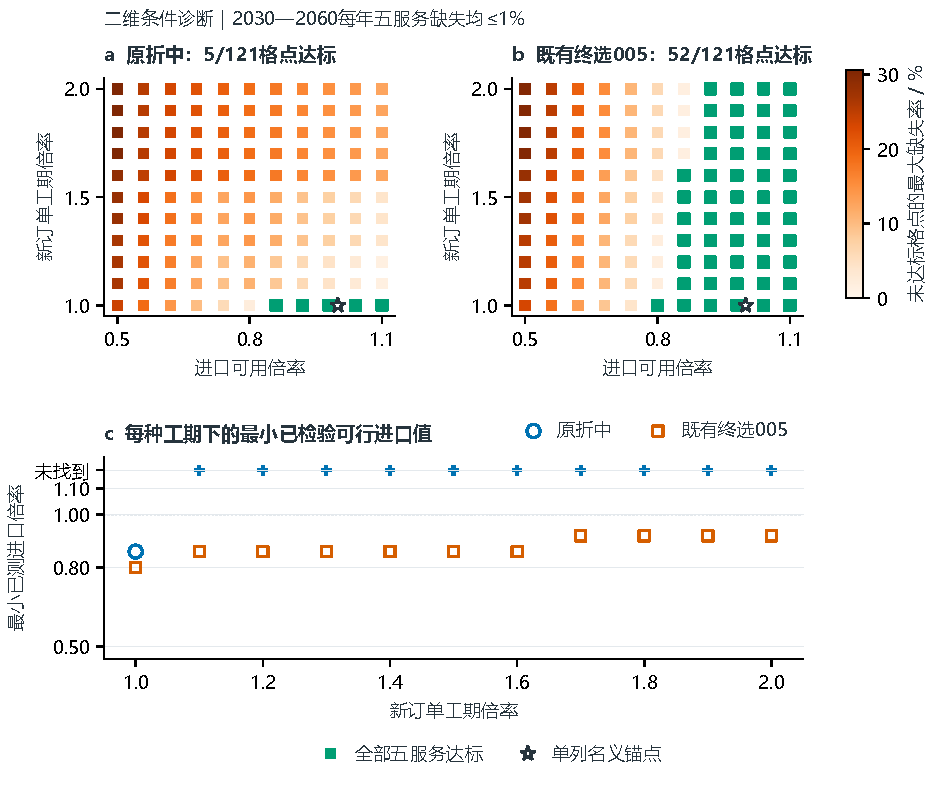
\includegraphics[width=160mm]{figures/figK_fixed_control_safety_envelope.pdf}
\caption{固定控制的进口—工期安全域。格点为实际测试组合，绿色满足2030—2060逐年五服务缺供$\le$1\%，橙色为最大缺失率；星号是单列名义锚点。下图仅连接每种工期最小的已测可行进口倍率，含工期1名义点；叉号表示已测试进口值中未找到可行点。}
\label{fig:fixed-control-envelope}\end{figure}

原折中在121点中仅5点达标，均为工期倍率1.00、进口倍率至少0.86的已测组合。保供修复（方案Ⅰ）增至52点：工期1.00的最小已测可行进口倍率为0.80，工期1.10—1.60为0.86，工期1.70—2.00为0.92。稳定非化石（方案Ⅱ）与方案Ⅲ分别为31、56点，形成不同资本与净排取舍。这里的点数衡量相同网格中的覆盖，图中标记用于选择已检验条件；两轴以外的条件仍由十维联合设计另行评价。

这一台阶直接对应油项目投产时点。对方案Ⅰ固定进口0.86，工期倍率从1.60增至1.70时，油新订单工期由5年取整为6年，2025年订单从2030年投产变为2031年投产；截至2030年，新订单形成的油能力由16.016降为0 Mtce/年，初始队列投产保持23.877 Mtce/年。2030年同为1195.631 Mtce的油请求，交付由1190.307降至1178.434 Mtce，缺失率由0.445\%升至1.438\%。保持工期1.70、将进口提高至已测0.92，油缺失归零且全部年份五服务达标，形成“投产台阶—油服务缺口—进口条件”的逐项见证。

进口增加不能代替全部建设。进口倍率1.10、工期2.00时，四个控制的2030年直接油服务均满足需求，但原折中仍在2031年出现12.44\%直接气缺失，稳定非化石（方案Ⅱ）仍在2030年出现2.72\%电力缺失。补充跨境料源可解除油供给约束，直接气与发电竞争、供给和电源建设兑现仍须共同检查。因此，早期油气交付先用渠道与订单时点核算，再按实际载能缺口配置电源；工程方案的适用条件应与资本和减排代价同时呈现。
进口倍率在本图中表示供给条件，表中资本为实际工程投资；保障额外进口能力的费用需另行核算。


\subsection{油气订单的有效建设窗口与2030年交付}
进口—工期网格揭示了投产台阶。进一步固定原保供修复方案及48组开发设计和名义条件，比较四种建设机制：P0为原提案与同比例支付；P1在油气不晚于2030年投产时优先付款；P2在有效窗口补至原物理建设上限并优先付款；P3全期均补至上限并优先付款。四臂共196条2025—2060年完整路径，在相同逐年预算金额下识别建设时点与组合结构的作用。

有效窗口由已知工期决定：$E_{f,t}=\mathbf{1}\{t+\lceil L_f d\rceil\leq2030\}$。油工期4、5、6年时，最后有效订单年分别为2026、2025、2024；气工期3、4年时分别为2027、2026。年建设上限、初始队列、退役、当期预算公式和进口演化沿用基准模型参数与演化方程。优先组资金不足时在组内按比例支付，剩余资金再分配给其他提案。本次四臂逐案逐年的实际预算金额相同，折现实付资本按实际订单另行累计。
\begin{table}[H]\centering\caption{建设时点机制的完整开发组与名义情景结果}
\begin{tabular}{lrrr}\toprule
机制 & 全年度可靠 & \shortstack{名义折现资本\\万亿元} & \shortstack{名义2060净排\\Gt}\\\midrule
原方案Ⅰ & 20/48 & 74.579 & 10.065 \\
有效窗口优先支付 & 20/48 & 74.579 & 10.065 \\
有效窗口补建设上限 & 20/48 & 74.936 & 10.076 \\
全期补建设上限 & 19/48 & 76.906 & 13.869 \\
\bottomrule\end{tabular}
\smallskip\par\noindent 可靠要求2030—2060各年电力、三种直接燃料及有效服务缺失均不超过1\%；48组为固定工程设计。
\end{table}
窗口优先支付在第38、39号设计增加气订单，第38号2030年气缺口降低0.419个百分点，但油缺口仍约24.396\%。窗口扩建P2在6组设计降低当年油缺口，完整年度可靠数仍为20/48；第32号原已达标，另五组仍未越过1\%门槛。全期扩建P3则降至19/48：高增长、低预算与进口收缩的第21号设计在2060年新增1.025\%电力缺失，折现资本由69.737增至71.075万亿元、净排由11.447增至14.471 Gt，以上差值均以原机制P0为参照。

第21号设计的全期油气扩建改变了共同资本配置和后续主体反馈。相对P0，2060年风光发电减少3158.661 TWh、煤电增加3687.398 TWh，总发电仍减少238.841 TWh；同时需求增加59.611 TWh，合成298.452 TWh电力缺口。局部燃料能力增长因此没有转化为全期可靠改善，应沿完整资产组合、实际投产和需求响应共同评价。

这一组负结果把措施落实到投产时钟：油工期6年时，2025年后的新订单均晚于2030；当期优先付款改变资金分配，却不改变既定工程周期。对具体年份的缺口，先核对已有队列、可在截止前形成的国内供给、进口和可释放库存，再确定建设与外部资源保障的组合。
\begin{figure}[H]\centering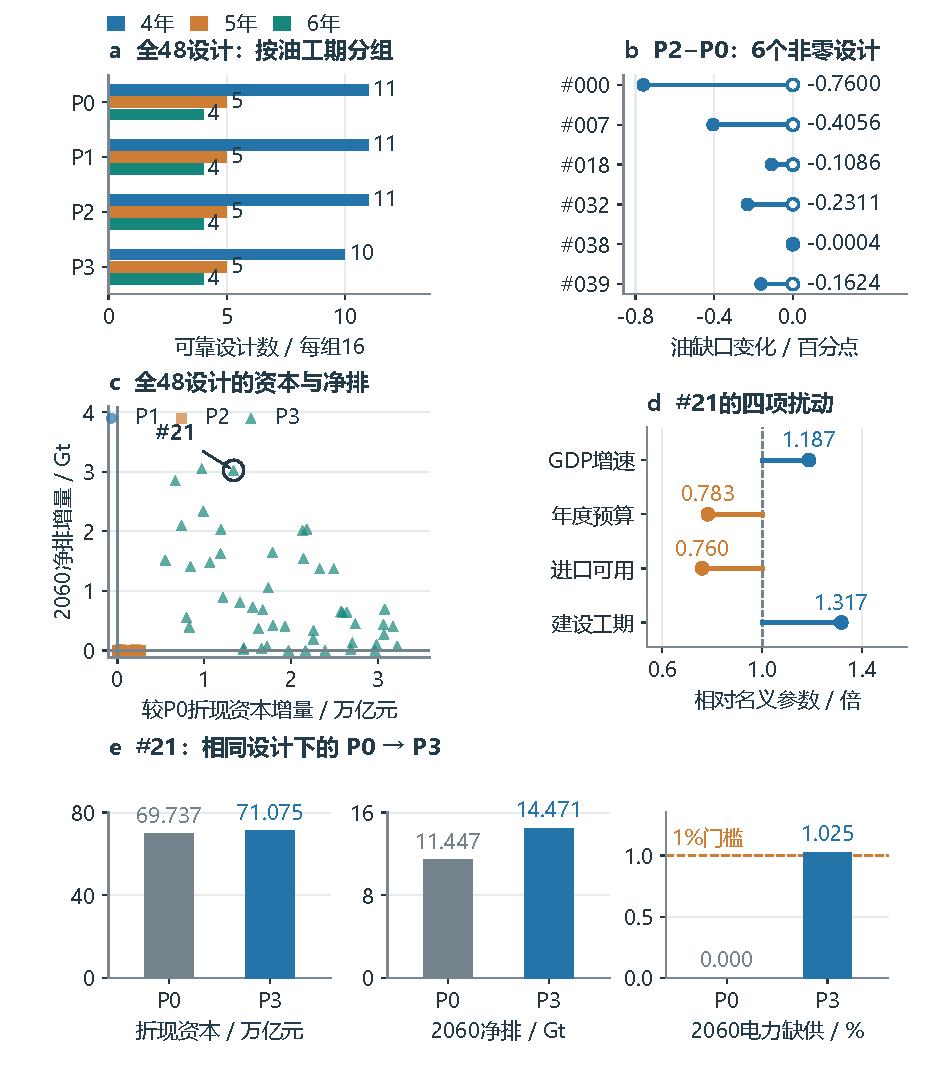
\includegraphics[width=\linewidth]{figures/figP_deadline_investment_mechanisms.pdf}\caption{建设时点机制的完整开发域比较。a按油工期分组，每组16个设计；全48设计可靠数为20/20/20/19。b显示P2相对P0油缺口的6个非零差，其余42组该指标为数值零。c保留全部48设计的资本—净排变化。d以名义值1标记第21号设计的四项扰动；e分别以完整坐标比较该设计P0与P3的资本、净排及电力缺供，1\%虚线为可靠门槛。资本按4\%、2024原点折现；净排和电力缺供取2060年度。}\end{figure}

\subsection{把年度投资组合落实到小时交付}
新增投资—运行、库存参照及运行条件试验统一采用SciPy/HiGHS逐时重优化，逐步反馈实际状态；原生实现证据在下一节单列。各轮协议和源程序在求解前固定，保存全部输入与逐时动作。

固定原折中、方案Ⅰ、方案Ⅱ和方案Ⅲ四个控制，将各自2030、2060年需求、装机、实际国内与进口料源流量和年末燃料库存传入同一360小时设计；每个快照各执行协调与原非化石局部储能规则，共16条完整路径、5760小时。方案Ⅰ使用实际年度原生复验输出，方案Ⅱ与方案Ⅲ由冻结控制重建年度轨迹；原折中2060的两条路径先逐列复现既有试验。各快照以50\%储能SOC、零热机记忆和零移峰债务初始化，之后连续反馈自身状态。该试验比较年度资产在相同工程事件中的交付，年度库存沿用各自轨迹，储能SOC采用统一设计初态。

\begin{figure}[H]\centering
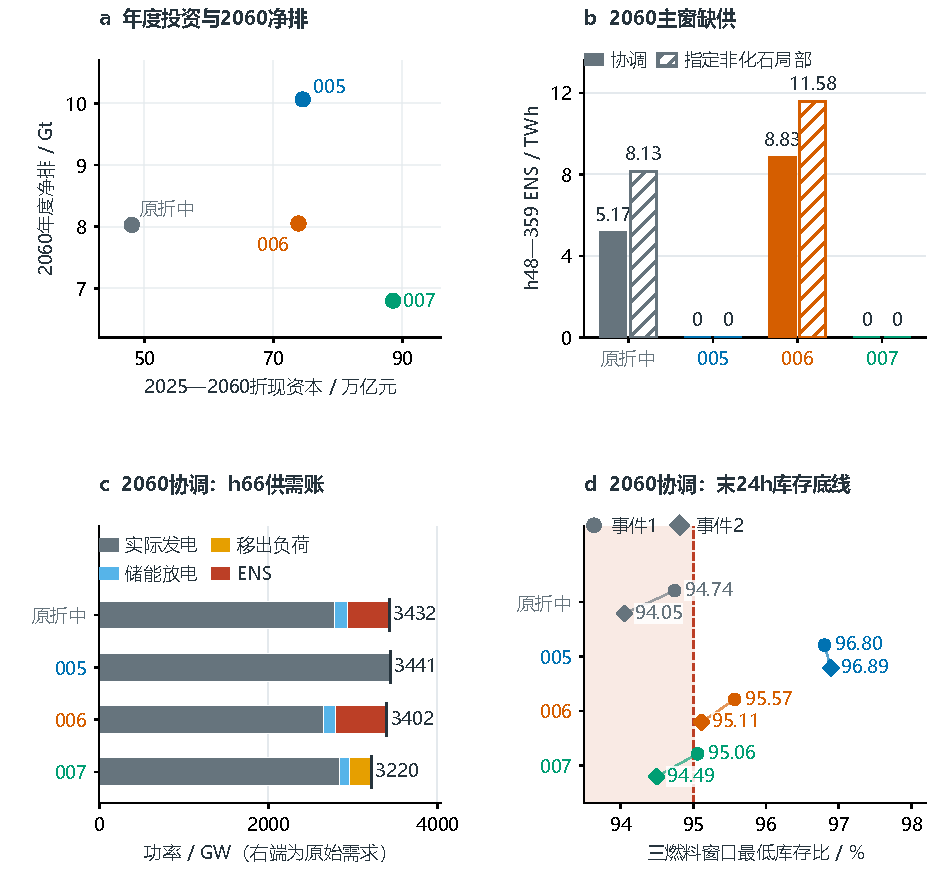
\includegraphics[width=160mm]{figures/figL_annual_operations_choice.pdf}
\caption{年度组合在小时层的实际交付。a为2025—2060折现资本与2060净排，b为h48—359缺供，c在共同h66核对供需；d为两次边界前24小时三燃料最低库存比，分母为各方案各事件前库存。2030八条路径主窗缺供均数值为零（绝对值$\le$$10^{-8}$GWh），完整360小时含预运行。}
\label{fig:annual-operations}\end{figure}
\begin{table}[H]\centering\caption{四个投资组合的协调运行：主评价窗与完整路径}
\begin{tabular}{lrrrrr}\toprule
组合 & \shortstack{2030主窗\\TWh} & \shortstack{2030全段\\GWh} & \shortstack{2060主窗\\TWh} & \shortstack{2060全段\\TWh} & \shortstack{2060主窗峰\\GW}\\\midrule
原折中 & 0.000 & 231.620 & 5.170 & 5.228 & 494.114 \\
方案Ⅰ & 0.000 & 224.241 & 0.000 & 0.188 & 0.000 \\
方案Ⅱ & 0.000 & 249.313 & 8.827 & 8.941 & 604.636 \\
方案Ⅲ & 0.000 & 96.235 & 0.000 & 0.000 & 0.000 \\
\bottomrule\end{tabular}
\smallskip\par\noindent 主窗为第48—359小时，全段为第0—359小时；小于$10^{-6}$ GWh的缺供按数值零展示，原始浮点值保留。
\end{table}

2060年方案Ⅰ与方案Ⅲ在主窗的电力缺供为数值零，方案Ⅱ为8.827 TWh，高于原折中的5.170 TWh。方案Ⅰ全360小时仍有187.839 GWh初始化缺供，四个2030快照的缺供也集中在初始化。年度服务达标与冲击交付因而须分别检验。

共同第66小时给出了组合差异的物理见证。方案Ⅰ需求3440.920 GW由实际发电完全覆盖，煤电出力2504.227 GW，距可用上限仍有244.887 GW。方案Ⅱ需求3401.528 GW虽低于原折中30.636 GW，发电可用上限却减少126.726 GW、储能交付功率减少14.432 GW；七类电源均达到当期上限，两储能仍有能量而触及放电功率上限，最终缺供604.636 GW，比原折中高110.521 GW。方案Ⅲ则以2844.383 GW发电、118.250 GW放电和257.620 GW负荷移出满足3220.253 GW需求。这些守恒账将资本转换为整套供给结构和时序动作，支持按实际缺口配置资产。

表中年度剩余净排以Gt计；小时燃烧CO$_2$与资源费用另行累计。2060协调完整360小时，原折中、方案Ⅰ、方案Ⅱ、方案Ⅲ的燃烧CO$_2$分别为439.721、473.313、428.412、390.363 Mt，资源费用分别为454.819、472.326、450.234、449.337十亿元。资源费含到货与净库存/SOC领用计价、运行和库存占用，不含缺供惩罚、碳价转移及新增工程资本。

\subsection{库存恢复采用三种参照回答三个问题}
方案Ⅰ在原事件前库存参照下，两次末24小时煤库存底线为96.80\%、96.89\%，两次服务与联合库存窗口均达标且随后保持；方案Ⅲ第二次底线为94.49\%，在第290小时再跌破。为进一步分离累积领用和事件增量，对上述16条冲击路径各增算一条同初态、同需求日型、同控制的无事件路径，共5760小时。新增路径只去除事件对可用出力、需求和进口的扰动。

定义$A_e=\min_{h\in W_e}S_h/S_{e,\rm pre}$，衡量相对最近事件前的恢复；$B_e=\min_{h\in W_e}S_h/S_0$，衡量相对试验初始储备的保持；$C_e=\min_{h\in W_e}(S_h/S_h^{\rm normal})$，衡量同小时无事件路径的资源差距。$W_e$取对应观察边界前24小时，$C_e$按逐小时比值取最小。原95\%恢复判定继续使用$A_e$，新增$B_e,C_e$用于解释库存演化。
\begin{table}[H]\centering\caption{2060协调路径第二次末24小时的煤库存及期末事件增量}
\begin{tabular}{lrrrr}\toprule
组合 & $A_2$/\% & $B_2$/\% & $C_2$/\% & \shortstack{期末额外领用\\Mtce}\\\midrule
原折中 & 94.05 & 88.95 & 91.95 & 30.461 \\
方案Ⅰ & 96.89 & 94.76 & 91.49 & 34.545 \\
方案Ⅱ & 95.11 & 90.93 & 92.14 & 30.303 \\
方案Ⅲ & 94.49 & 89.72 & 92.08 & 30.160 \\
\bottomrule\end{tabular}
\smallskip\par\noindent 额外领用为无事件期末库存减冲击期末库存；三列比例分别采用事件前、固定初始和同小时无事件库存作为分母。
\end{table}

方案Ⅰ相对最近事件前已恢复，但相对固定初始库存的第二次窗口底线为94.76\%，相对同小时无事件库存为91.49\%。其期末煤库存为372.181 Mtce；无事件路径本会累积至406.726 Mtce，两者相差34.545 Mtce。原折中相应事件增量为30.461 Mtce。三种参照共同表明：方案Ⅰ改善了供给组合与相对事件前的准备，持续资源保障还须计入正常演化的库存目标。原库存费用已包含资源净领用，表中额外领用按实物量报告。

\subsection{补库购买了哪些准备：现金、资源与目标分账}
在四个2060资产组合上各比较继承原到货与原付费应急合同，共8条360小时完整路径。合同按预定事件日历，在事件结束12小时后追加进口；总流量最高为原年进口能力折小时的150\%，因而需要额外通道余量。三燃料新增到货分别为煤10.623、油23.553、气6.046 Mtce；每条路径的非库存动作、缺供、峰值与CO$_2$均与对应原到货路径相同，增量到货全部留为期末库存。

每方案新增采购现金为1666.523亿元，其中基价1111.016亿元形成新增期末燃料资产，溢价555.508亿元构成物理资源净增费。沿用同一工程单位价值，采购现金与资产形成分别列账；运输扩容资本和融资费用另需工程项目数据。

以最近事件前库存为参照A，原折中与方案Ⅲ的第二次窗口由未持续达标转为达标，首次联合确认时刻仍为119、263小时。以固定初始库存为参照B，合同后的四方案第二次窗口最低比率依次为91.601\%、97.223\%、93.526\%、92.306\%；以原继承到货、无事件资源路径为参照C，依次为94.440\%、93.800\%、94.583\%、94.553\%。A回答相对最近事件前的恢复，B回答期初资源保持，C回答原无事件资源目标下的准备程度。该合同增购准备，原资源目标仍给出后续补充量。
\begin{figure}[H]\centering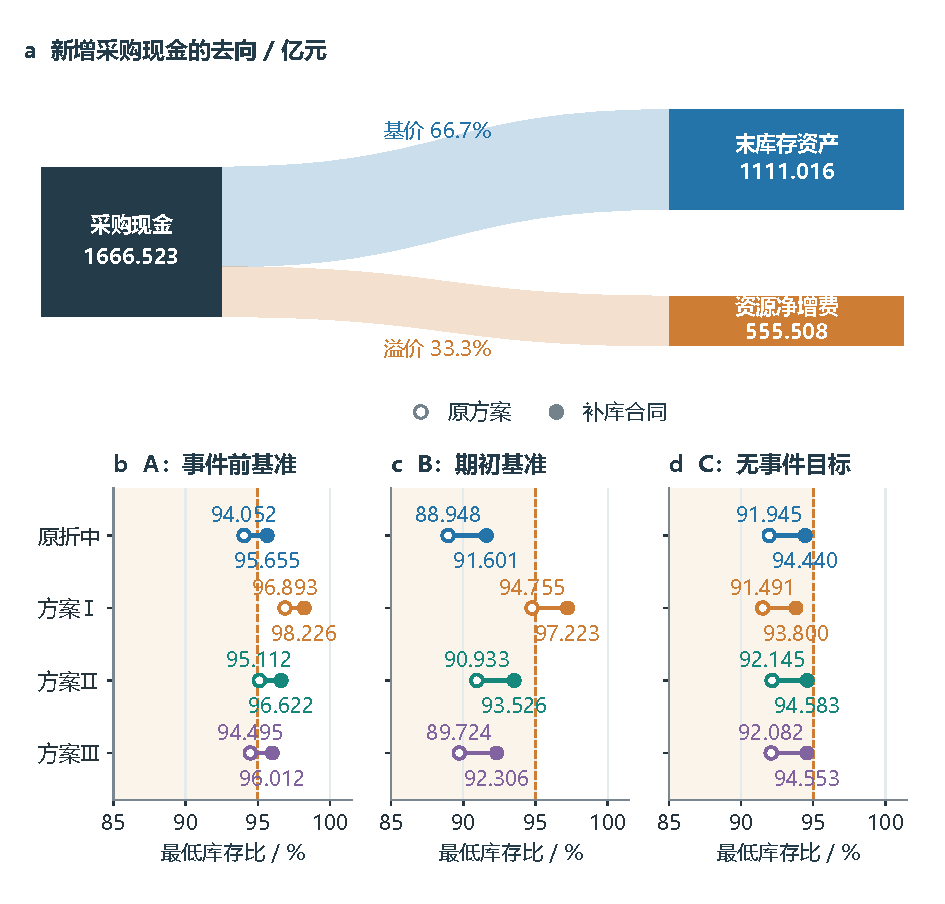
\includegraphics[width=\linewidth]{figures/figN_replenishment_cash_and_readiness.pdf}\caption{补库的现金分解与资源准备。a按实际金额比例将1666.523亿元采购现金分为1111.016亿元新增末库存资产和555.508亿元溢价，后者等于物理资源净增费；基价不重复计入资源净耗费。b—d显示h336—359逐燃料、逐小时库存比最低值，空心原方案→实心合同。A、B、C分别以自身事件前库存、自身期初库存及相同资产下原无事件资源路径为参照；95\%虚线为相应参照值。}\end{figure}

\FloatBarrier

\section{原生协同仿真与冲击恢复}
\subsection{原生模型实现与分层验证}
原生Simulink资源网络将“提出动作”和“更新状态”分开执行。控制器根据上期库存、SOC、机组出力记忆与共同24小时输入求解18项动作；原生Sum、Gain及Unit Delay模块计算本小时物理交付和下一小时状态。煤、油、气库存分别加入到货、扣除实际直接服务和发电领用；两类储能分别计算充放电效率损失；移峰债务和机组爬坡记忆持续继承\cite{mathworks_step}。

\begin{figure}[H]\centering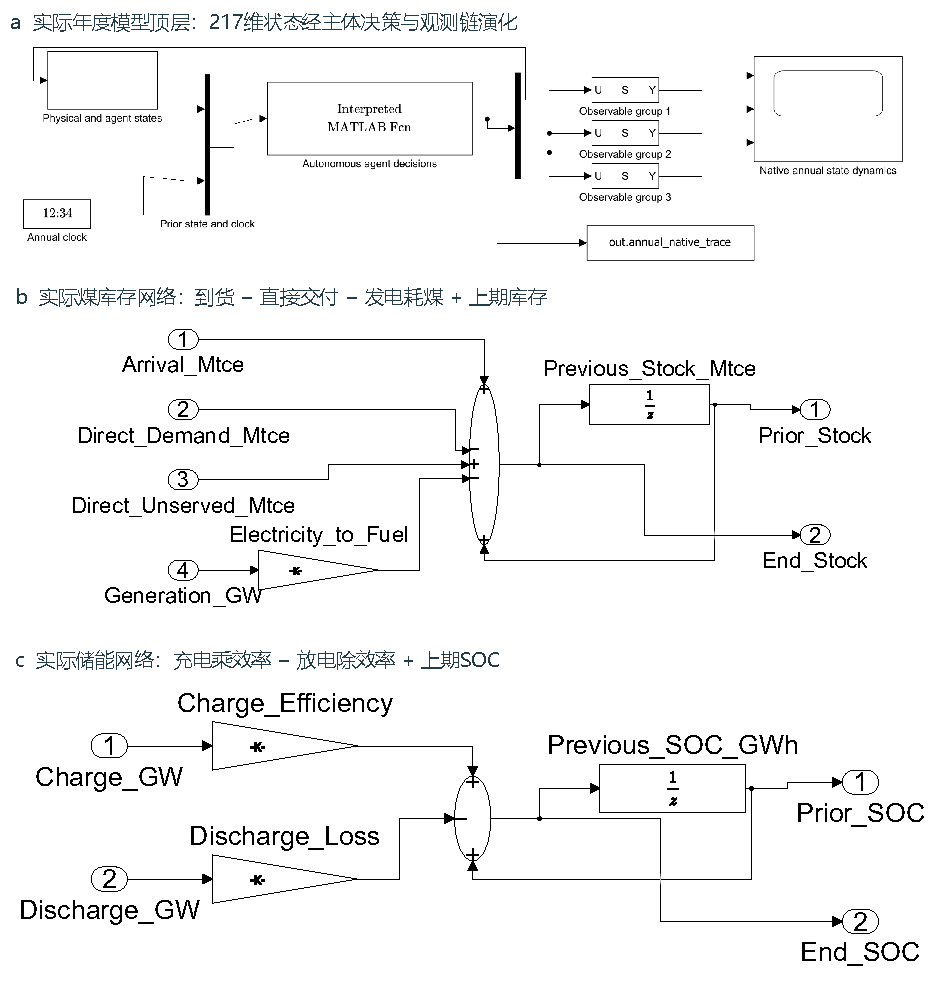
\includegraphics[width=\linewidth]{figures/native_v9_resource_conservation.pdf}\caption{实际Simulink工程的全景与守恒局部。a为年度217维状态模型的真实顶层封装，主体与12类资产15槽队列在决策函数内实现；b—c为煤库存与储能的原生矢量导出，分别按G/(8141$\eta$) Mtce/小时和$\eta_c$·充电$-$放电/$\eta_d$更新。中文说明位于原图外，Unit Delay保存上一小时状态。}\end{figure}

新物理网络在继承供应和付费补库下分别连续执行2160小时，与已执行输出逐列核对49个通道，并从导出CSV独立重建电力、燃料、SOC与债务账；最大电力平衡残差为$1.23\times10^{-11}$ GW。年度实现另对15组状态演化核对。新增保供修复（方案Ⅰ）在相同Simulink年度模型中实际完成2025—2060年演化，仅输入观察初态、固定参数与常量政策，由原生模型逐年产生217维状态和12类投资动作。36年共7,812个状态值、4,752个原始指标及432次投资动作与独立Python实现核对，最大归一化差为$3.64\times10^{-12}$；建设队列移位、投产与退役逐项相符，三燃料、电力及资本账独立闭合。该实现检验与前述历史误差分别报告：前者检查状态方程和实现，后者检查历史资料下的组件表现。

\begin{table}[H]\centering\caption{历史诊断、物理验证与原生实现的分层检验}
\begin{tabularx}{\linewidth}{p{.19\linewidth}XX}\toprule
检验层次 & 方法与对象 & 已完成证据\\\midrule
历史与行为 & 各训练起点以前资料校准共享预期及资产组件，条件给定已实现GDP & 一年/三年电力MAPE为1.713\%/3.992\%；近期净增基线为2.306\%/2.452\%\\
数学与物理 & 逐时平衡、库存、SOC、爬坡及负荷债务；线性规划原域与对偶条件 & 电力平衡最大残差$1.23\times10^{-11}$ GW；联合约束与末态证书按实际成功记录核查\\
软件实现 & MATLAB/Simulink与Python年度状态；AnyMath与Python各自闭环 & 年度最大归一化差$3.64\times10^{-12}$；1800个小时缺供差最大$2.3\times10^{-13}$ GW\\
\bottomrule\end{tabularx}\end{table}
各组对照采用相同初态和声明的信息条件，先用既有路径核对实现，再完整执行固定比较组；输入、原始结果与全部失败状态列于附录及支撑材料。年度控制在48组开发设计中选择，另48组拉丁超立方设计以种子20261019独立生成，控制固定后只检验一次，未据此再调参。工程设计范围与历史误差、软件一致性分别解释。

\subsection{AnyMath参数干预、小时重优化与连续恢复}
AnyMath实现采用“读取原生状态—求解24小时协调问题—执行首小时动作—原生网络推进状态”的循环。Julia/HiGHS在每小时重新优化发电、两类储能、移峰及未满足服务等18项动作，原生Sum、Gain和Unit Delay网络计算三燃料库存、两储能SOC、移峰债务及两机组记忆；下一次优化读取这些原生末状态\cite{anymath_docs}。修改冲击强度、持续时间、补库方式或储能功率后，从同一初态建立新会话，旧轨迹保留其参数身份。

为直观展示两次冲击与中间恢复，另设360小时工程设计：冲击区间为$[48,96)$与$[192,240)$，合同在冲击退出12小时后开始补库；系统采用折中2060快照。短设计与前述2160小时试验分别覆盖不同事件持续期，缺供和恢复结果各按所属设计报告。五组参数均在平台内完成360次逐时优化与原生状态推进，共享24小时完美前瞻，求解状态逐小时导出。

\begin{figure}[H]\centering
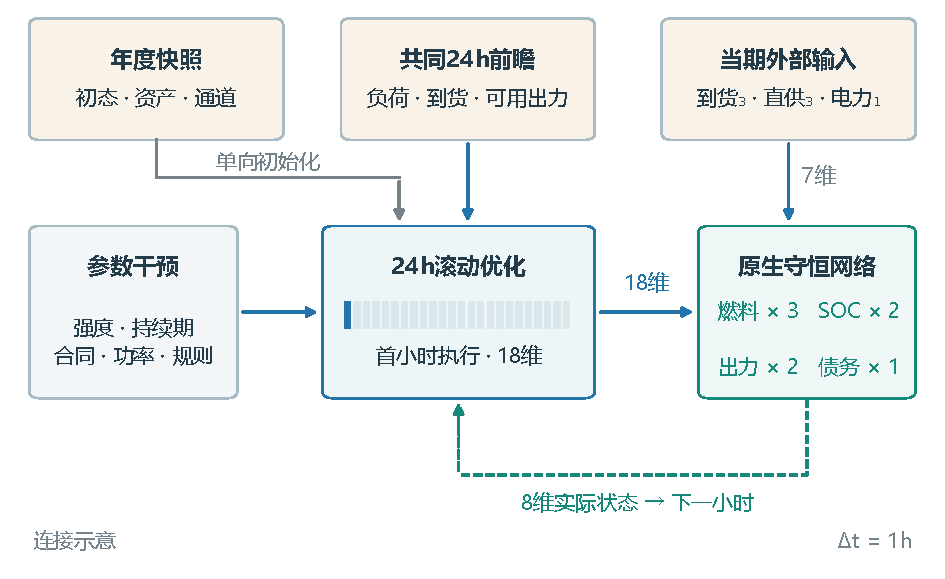
\includegraphics[width=\linewidth]{figures/native_closed_loop.pdf}
\caption{已实现小时系统的分层连接。年度快照单向提供初态、资产和通道能力，优化器与原生网络使用同源初态；共同24小时前瞻进入滚动优化，只执行首小时18维动作。7维当期外部输入与动作进入原生守恒网络，三燃料库存、两类SOC、两类热机出力记忆及一项移峰债务共8维实际状态反馈至下一小时，步长1h。此图为连接示意；箭头宽度不表示流量。}
\label{fig:native_closed_loop}\end{figure}

\begin{figure}[H]\centering
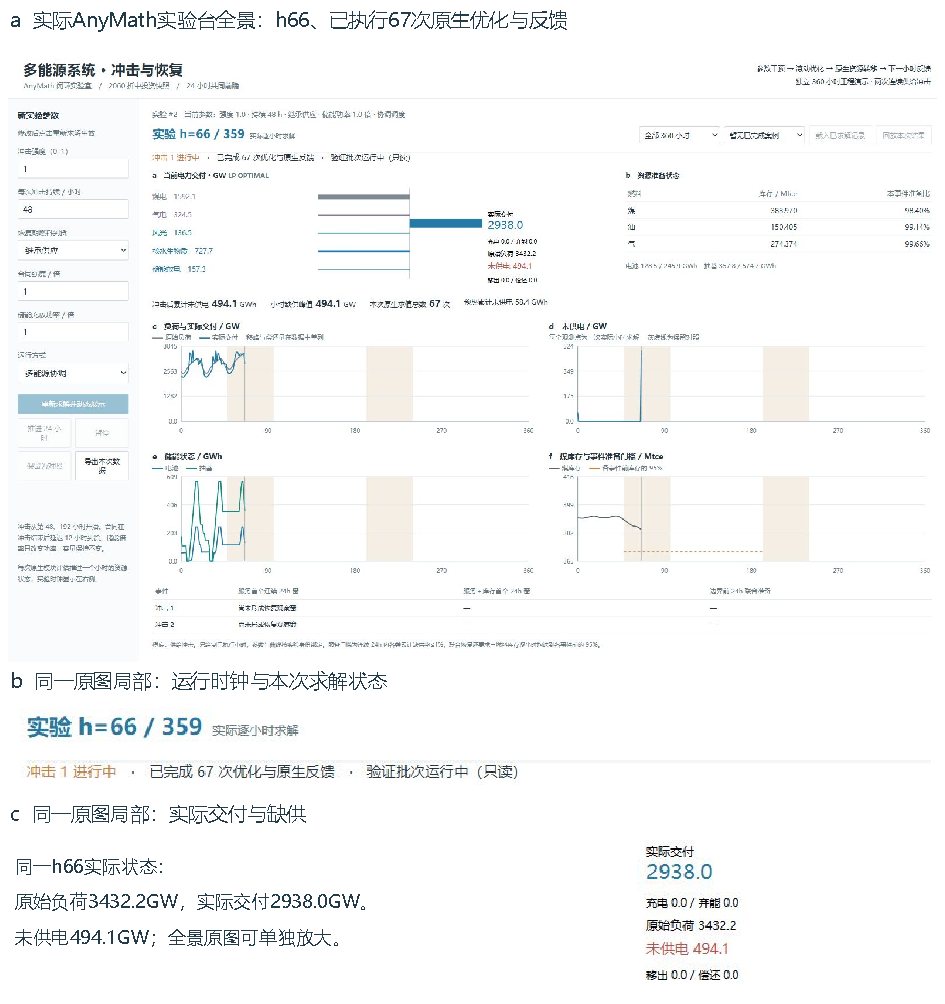
\includegraphics[width=\linewidth]{figures/native_anymath_v10_live.pdf}
\caption{同一h66的AnyMath真实全景与局部放大。参数控制、能流、库存/SOC、六视图和恢复表来自同一原图；b显示h66/359及已执行67次优化与原生反馈，c显示实际交付2938.0GW和缺供494.1GW。全景未拼接不同时刻，原始高清图随支撑材料提供。}
\label{fig:anymath_v10_live}\end{figure}

\begin{table}[H]\centering\caption{AnyMath闭环设计实验的实际结果（均为360小时全段）}
\begin{tabular}{lrrr}\toprule
方案 & 未供电/TWh & CO$_2$/Mt & 资源费/亿元\\\midrule
协调基准 & 5.228 & 439.7 & 4,548.2 \\
减轻冲击 & 0.058 & 393.7 & 4,350.6 \\
提高储能功率 & 5.170 & 436.3 & 4,548.5 \\
合同补库 & 5.228 & 439.7 & 5,103.7 \\
分散策略 & 8.192 & 440.9 & 4,548.6 \\
\bottomrule\end{tabular}\end{table}
\noindent 资源费按到货、库存领用、非化石运行、储能、移峰、库存持有与合同溢价记账，不含缺供惩罚、碳价转移及增功率工程投资。未供电含初始化阶段，前述2160小时剔除预热的指标另行报告。

\textbf{提高功率改变缺口时序，补库改变跨事件资源准备。}在能量容量不变时，将储能功率提高50\%，第66小时两类储能多交付78.634 GW，主窗缺供峰值由494.1降至415.5 GW。峰后缺口回补与削峰改善各为0.681 TWh，主窗累计未供电仍为5.170 TWh；全段减少的0.058 TWh来自前48小时初始化。因此，峰值改善与累计能量改善应分别核算。

应急合同在冲击退出12小时后开始追加到货，期末煤库存增加10.623 Mtce，而全段缺供仍为5.228 TWh。这一对照表明，新增资源在本组事件中主要转为库存准备，不能仅由采购量推断电力增发；其作用应继续沿恢复窗口和事件边界检验。

联合恢复须在连续24小时内满足各服务合计缺供率不超过1\%、三库存逐小时不低于事件前95\%。以下按本次条件轨迹比较首次确认、再跌破和观察边界，未确认者保留右截尾。

第1次冲击后，协调基准在第119小时确认首个合格窗口，又在第146小时重新跌破库存门槛。到观察边界，基准与合同方案的煤库存分别为各自冲击前的94.74\%和95.93\%；最后24小时联合准备分别为未达标与达标。

第2次冲击后，协调基准在第263小时确认首个合格窗口，又在第269小时重新跌破库存门槛。到观察边界，基准与合同方案的煤库存分别为各自冲击前的94.05\%和95.72\%；最后24小时联合准备分别为未达标与达标。

在本次条件轨迹中，合同补库使两次观察边界的联合准备均转为达标，累计未供电保持不变；资源准备与当期电力交付分别响应不同约束。


\begin{figure}[H]\centering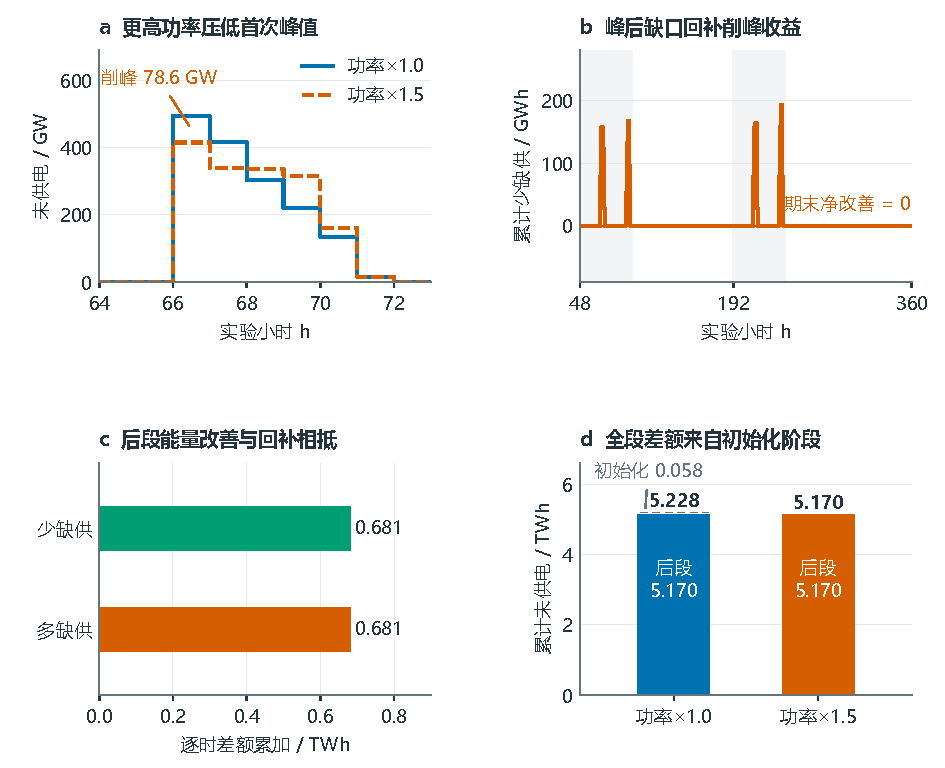
\includegraphics[width=\linewidth]{figures/figI_power_energy_accounting.pdf}
\caption{储能功率与能量缺口的分离。放电功率增加改变逐时缺口分布，后段缺供增减能量相互抵消；初始化阶段另列，全部功率与能量保持相应单位。}\label{fig:figI_power_energy_accounting}\end{figure}

\subsection{恢复定义与完整路径检验}
固定已执行轨迹，将连续窗口设为12、24、48小时，库存门槛设为90\%、95\%、99\%，各服务缺失门槛设为0.5\%、1\%、2\%，共重算270个事件定义。默认定义逐项复现原10个事件，计算前后调度动作保持原值。定义$\kappa_{e,W}=\min_{h\in[T_e-W,T_e),f}S_{f,h}/S_{f,\mathrm{pre}}$，其中$T_e$为事件观察边界，$S_{f,\mathrm{pre}}$为该次冲击前库存；$\kappa$即边界前$W$小时所有燃料的最小库存比。在服务合格时，库存要求不超过$\kappa$即可维持该窗口准备。

两次事件的24小时库存底线，基准分别为94.74、94.05\%，合同分别为95.82、95.65\%。95\%要求处于两方案的分界区间，区分了当期服务与持续准备；90\%和99\%规则分别对应更宽松和更严格的资源要求。

另以独立SciPy/HiGHS新执行五条各360小时完整闭环路径，两实现各自反馈本实现的实际状态。1800个逐小时缺供差的最大值为$2.3\times10^{-13}$ GW，累计缺供及10个事件的默认恢复判定、再跌破时刻一致。两实现的SOC、机组输出与偿还时点存在分支；这组完整路径比较与同状态最优目标核验共同支持本组服务和准备结论，实际轨迹仍保留其求解器身份。

\subsection{用更强的局部规则识别协调的增量价值}
原分散规则以需求减非化石可用出力形成储能净负荷，正值放电、负值充电。冲击期间，非化石出力不足使其难以利用煤气电余量充电。为检验协调在更强规则下的作用，增加“可达全电源余量局部”规则：以当期真实热机记忆出发，逐时按爬坡和可用上限递推煤气电可达出力，连同非化石可用出力计算储能净负荷；沿用原贪心储能顺序、效率和SOC约束，再由同一市场调度器执行。该规则使用同样24小时前瞻、资产、外部输入和资源账。
\begin{table}[H]\centering\caption{更强局部规则与协调的完整路径比较}
\begin{tabular}{lrrrr}\toprule
规则 & \shortstack{主窗缺供\\GWh} & \shortstack{主窗峰\\GW} & \shortstack{全段资源费\\十亿元} & \shortstack{全段CO$_2$\\Mt}\\\midrule
协调/原功率 & 5169.910 & 494.114 & 454.819 & 439.721 \\
可达余量局部/原功率 & 5279.366 & 494.114 & 459.893 & 447.447 \\
协调/1.5倍功率 & 5169.910 & 415.480 & 454.845 & 436.283 \\
可达余量局部/1.5倍功率 & 5222.077 & 415.480 & 460.277 & 444.789 \\
指定非化石局部/原功率 & 8133.428 & 651.383 & 454.855 & 440.877 \\
\bottomrule\end{tabular}
\end{table}
原功率下，协调相对可达余量局部规则减少缺供109.455 GWh（2.073\%）；1.5倍功率下减少52.167 GWh（0.999\%），两组各自的峰值相同。36.4\%的原结果对应指定非化石局部规则，更强基线下的增量来自联合安排储能、发电与负荷偿还。原功率/1.5倍功率下，协调资源费分别少50.737/54.324亿元、燃烧CO$_2$少7.726/8.506 Mt。终态也随策略改变：协调末SOC接近零，可达余量局部规则末电池与抽蓄均充满，合计820.638 GWh；费用已按相同0.32百万元/GWh计入SOC净领用，燃料库存另按同一价格计价。费用和排放随实际轨迹比较，终态准备程度由独立库存与SOC账同时呈现。

\subsection{相同期末储能电量下，协调收益仍保留}\label{sec:common-terminal}
原比较的协调路径期末储能接近零，强本地规则期末充满。保持四种控制与全部外部输入，新增共同终点要求：第360小时边界，电池与抽蓄均达到各自满容量，合计820.638 GWh。仅在滚动窗口触及真实终点时改变两个末SOC边界；

共同终点的干预仅在最后24小时进入规划，四臂第0—335小时全部状态与动作逐值相同。两条强本地路径全程不变；两条协调路径在后段减少放电并增加充电，额外煤气发电分别为774.727、791.650 GWh，完整路径缺供均不增加。电池和抽蓄电量统一后，实际燃料库存与热机出力继续逐项报告。
\begin{table}[H]\centering\caption{共同满电终点下，强本地规则减协调的配对差}
\begin{tabular}{lrrrr}\toprule
功率条件 & \shortstack{主窗缺供\\GWh} & \shortstack{主窗峰值\\GW} & \shortstack{全段物理费\\亿元} & \shortstack{全段CO$_2$\\Mt}\\\midrule
原功率 & 109.455 & 数值零 & 50.750 & 7.088 \\
1.5倍功率 & 52.167 & 数值零 & 54.007 & 7.891 \\
\bottomrule\end{tabular}
\smallskip\par\noindent 主窗为h48—359，全段为h0—359；峰值原始差约$5.7\times10^{-13}$ GW，展示阈值$10^{-8}$ GW。
\end{table}
原功率与1.5倍功率下，协调的缺供、物理资源费用与CO$_2$改善均保留，峰值各自相同。物理费沿用燃料到货与净库存、非燃料运行、储能循环、移峰、SOC净领用及库存持有账。共同终点使原SOC净领用估值项减少262.604百万元；两协调路径的其他运行资源费增加261.344、294.261百万元，净物理费分别变化$-1.260$、$+31.656$百万元。增购末电量形成资产，运行补电支出与净资源费据此衔接。
\begin{figure}[H]\centering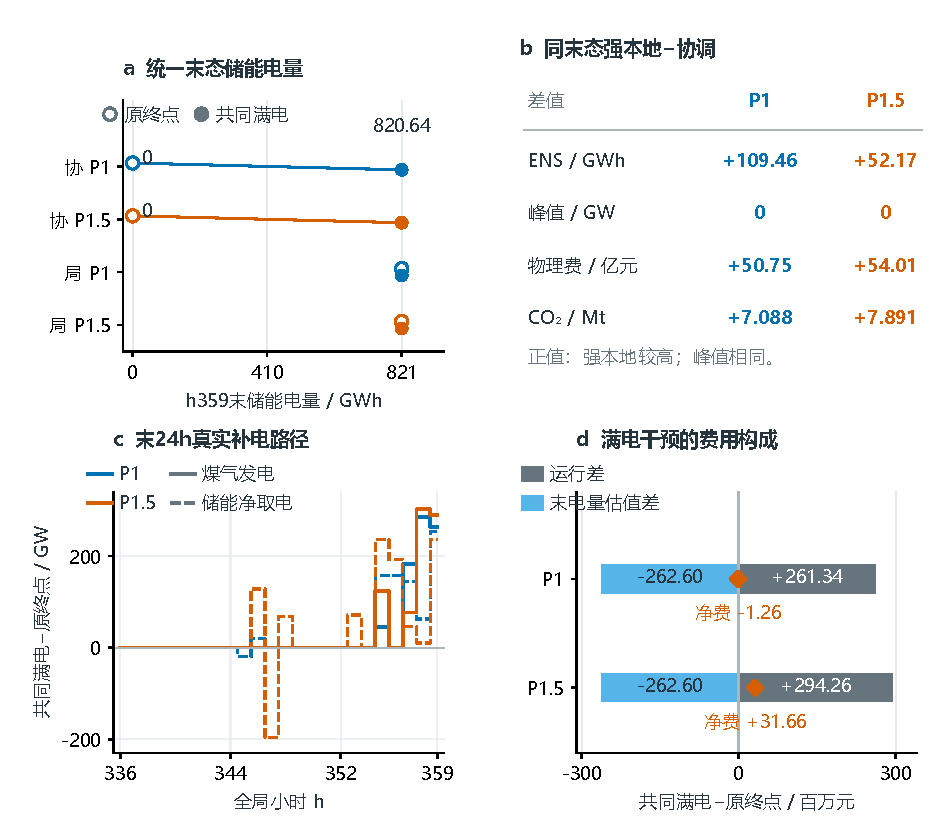
\includegraphics[width=\linewidth]{figures/figO_common_terminal_storage.pdf}\caption{共同满电终点下的实际补电、收益与计价。ENS和峰值取h48—359，费用及排放取完整360小时；共同满电约束进入h336—359。两功率仅P不同，能量容量、初始50\%电量和24小时前瞻相同；费用含0.32百万元/GWh末电量净领用估值，不含缺供罚金和碳价，末燃料与热机出力仍可不同。}\end{figure}

\subsection{事件信息改变动作与费用，服务结果另行检验}
保持24小时优化窗口和正常工程日型已知，只改变事件状态的可见时长$L=1,6,24$小时；超过可见部分，以最后一个已知事件状态延续。真实执行始终使用实际当小时事件，三条原策略各执行三种信息条件，共9条360小时路径。每条路径继承自身实际库存、SOC、爬坡记忆与债务，常态日型与事件预见性分别设置。

三种信息条件下，各原策略主窗累计缺供和峰值数值一致；动作并未全部相同。$L=1$相对24小时，协调、增功率协调和指定非化石局部规则分别有41、44、14个小时动作改变，全段资源费用分别增加1.544、2.464、1.619亿元。协调首次库存再跌破由第146小时前移至第145小时，服务窗口仍在第119、263小时确认。该组瓶颈限制了服务指标对信息变化的响应，信息价值同时体现在实际动作、资源领用与准备时点上。

\subsection{完整事件设计给出动作的优势区间}
固定上述五条控制器，以相位$\phi\in\{0,3,6,9,12,15,18,21\}$小时、事件持续期$d\in\{12,24,48,72\}$小时组成32个格点。两次冲击从$48+\phi$、$192+\phi$开始，其他事件强度、进口和需求扰动、360小时时轴及24小时前瞻保持原值。每格完整执行五条路径，160组共57,600小时；相位同时改变冲击与负荷/风光日型、绝对偿还时点的相遇关系，持续期改变事件剂量，因而各格用于工程设计条件的比较。

\begin{figure}[H]\centering
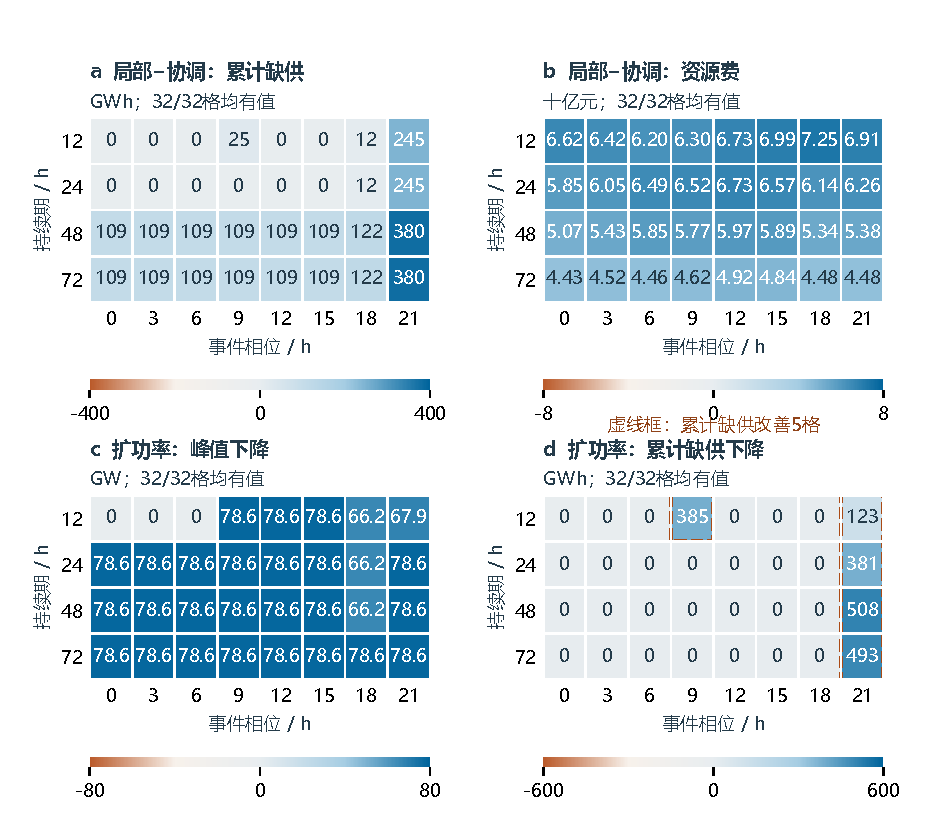
\includegraphics[width=160mm]{figures/figM_event_advantage_domain.pdf}
\caption{32格事件条件下的完整优势域。a—b为原功率下可达全电源余量局部减协调；c—d为协调原功率减1.5倍功率，能量容量不变。虚线框仅标5个累计缺供改善格，27格为有效数值零，不能统一解释为已达夜间守恒下界。主窗h48—359；各面板单位内绝对差$\le$$10^{-8}$显示0，原值128格完整保留，费用含净库存与SOC领用估值。}
\label{fig:event-advantage}\end{figure}

对可达余量局部规则，原功率协调在21/32格减少主窗缺供、11格数值相同，改善范围0—379.620 GWh；1.5倍功率下分别为19格改善、13格相同，改善0—422.201 GWh。原功率32格资源费均下降44.296—72.539亿元、燃烧CO$_2$少5.041—11.331 Mt，终态SOC差保持上述方向。全部格点展示了收益的大小与条件。

增加50\%储能功率在29/32格削减小时缺供峰值，最大78.634 GW；累计缺供仅在5/32格减少，范围0—508.270 GWh，另外27格数值相同。5个改善格为相位9小时/持续12小时，以及相位21小时/持续12、24、48、72小时。相位9、持续12小时格在第66—68小时多交付192.538 GWh；冲击第69小时结束后，可用能力盈余足以偿还负荷，额外交付得以保留为累计改善。原相位0、持续48小时格则将同一可用储能能量重新分配，主窗缺供总量相同。功率扩充能否进一步减少能量短缺，取决于功率受限时仍有可用能量，以及事件退出后能否无新增缺供地偿还先前负荷。各格的改善比例用于这32种设计条件，事件发生概率需由独立资料建立。

\subsection{储能时长依据与单参数挑战}
国家能源局报告给出2024年底新型储能73.76 GW、168 GWh、平均2.3小时，统计涵盖多种新型储能技术\cite{nea_storage_2025}。本文基年采用73.76 GW功率，并以4小时电池、6小时抽蓄作为工程配置；4小时也属于NREL储能技术经济比较的代表配置\cite{nrel_atb_storage}。为检验能量配置对运行结论的影响，固定折中2060资产和全部控制，将电池容量从原功率乘4小时改为原功率乘2.3小时，初始SOC仍为各自容量的50\%。同一时长内增加功率保持能量容量不变，抽蓄保持6小时；五规则各执行两时长，共10条完整路径、3600小时。
\begin{table}[H]\centering\caption{电池时长变化下的主窗缺供}
\begin{tabular}{rrrrr}\toprule
\shortstack{电池时长\\h} & \shortstack{协调原功率\\GWh} & \shortstack{可达局部原功率\\GWh} & \shortstack{协调1.5倍\\GWh} & \shortstack{可达局部1.5倍\\GWh}\\\midrule
4.0 & 5169.910 & 5279.366 & 5169.910 & 5222.077 \\
2.3 & 5566.564 & 5676.019 & 5566.564 & 5618.731 \\
\bottomrule\end{tabular}
\end{table}

电池由4小时减为2.3小时，协调在两种功率下主窗缺供均增加396.654 GWh，约为主窗原始需求的0.0434个百分点；两种功率协调的峰值仍为494.114/415.480 GW，累计缺供仍相同。2.3小时下，协调相对可达余量局部规则依然分别少缺供109.455/52.167 GWh；在1.5倍功率下还将峰值由465.778降至415.480 GW，较少可用能量使规则间的削峰差异显现。能量配置影响累计交付，功率配置影响逐时交付，两者在本组设计中分别显现。该试验只改变小时电池能量与其初始SOC，年度投资路径和资本费用继续按原组合报告。

\subsection{累计缺供的离线最优参照与剩余调度空间}
固定相位0/21小时、原功率/1.5倍功率、末SOC自由/共同满电八组条件，每组先复现24小时滚动路径，再固定其实际前48小时，从第48小时完整状态一次优化剩余312小时。原燃料、爬坡、容量、效率及13个绝对日末偿债条件全部保留，三种直接燃料服务全额交付。该离线参照同时获得真实后续输入并改变优化方式，用于识别固定资产下的可达边界。

先最小化累计缺供$U$，再在$U\le U^*+10^{-6}$ GWh下最小化物理资源费。8条滚动与8条离线共执行5760小时实际状态转移、2896次LP；原矩阵、解与对偶全部保存。八组滚动缺供与第一阶段最小值均数值相同，滚动值与对偶下界的最大绝对间隙小于$1.2\times10^{-11}$ GWh。第二阶段增加的约1 kWh来自预定容差。

\subsection{用四段夜间守恒解释能量瓶颈}
对结束于绝对日末的窗口$W=[a,b)$，债务$Z_b=0$、$Z_a\ge0$给出$\sum_W(repay-out)=Z_a\ge0$。储能满足$S_b-S_a=\eta_c\sum ch-\sum dis/\eta_d$，结合$0\le S\le E$与$\eta_c\eta_d\le1$，得到$\sum_W(dis-ch)\le\eta_dE$。再用发电可用上限$A$及电力平衡，得到
\begin{equation}
\sum_{t\in W}ENS_t\ge\left[\sum_{t\in W}\left(D_t-\sum_gA_{g,t}\right)-\sum_s\eta_{d,s}E_s\right]_+.
\label{eq:night-cut}
\end{equation}
每窗允许从满电开始，已放宽了真实燃料、爬坡与前期充电限制；四个互不重叠窗口的下界可以相加。图\ref{fig:energy-cut}把可用发电后的总缺口拆成最多可交付储能与不可消除的缺供。

\begin{figure}[H]\centering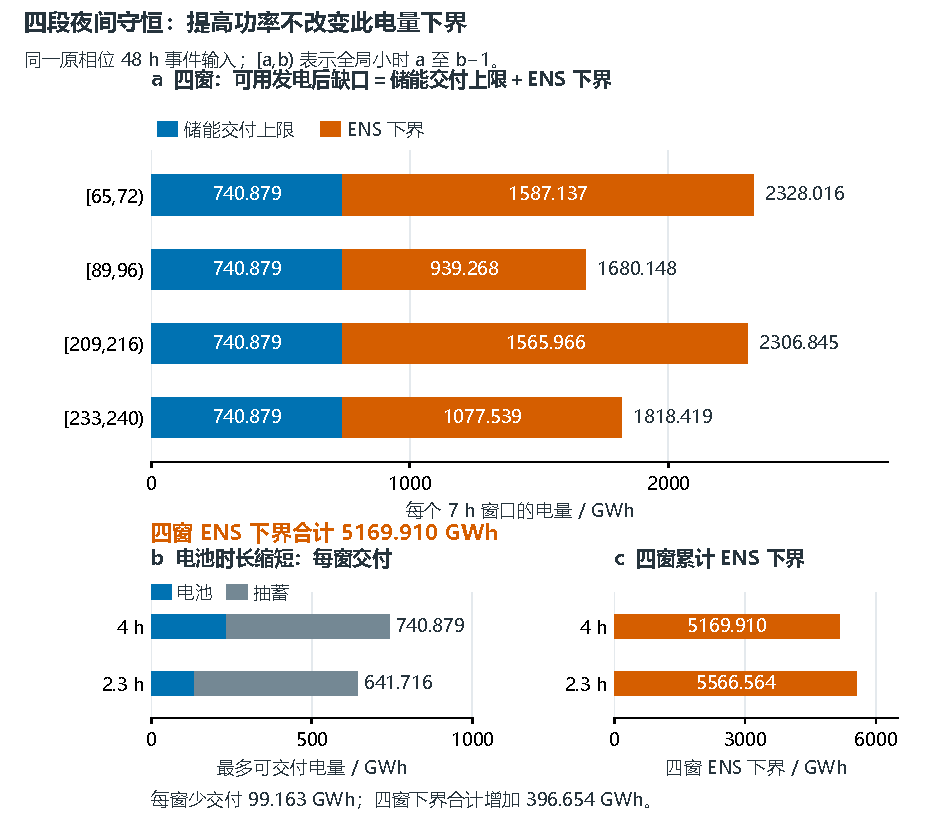
\includegraphics[width=160mm]{figures/figR_energy_conservation_floor.pdf}
\caption{原相位四段夜间的能量守恒下界。四个不重叠7小时窗均结束于日末偿债点，每窗允许满电开始，最大储能交付$\sum_j\eta_{d,j}E_j$；移峰不能净移出窗口。下界合计5169.910GWh，功率增加50\%而E不变时下界不变；电池由4小时减至2.3小时使四窗交付减少396.654GWh。结论限该原相位、既定容量与日末偿还规则，完整14路径56窗另表。}\label{fig:energy-cut}\end{figure}

这一结果解释了原48小时设计：调度已到达累计电量边界，增加功率仍可改变缺口的小时分布，增加可交付能量才可能下移该边界。32格事件试验中的5个能量改善格则具有不同的功率受限与事后偿还条件，按各自实际路径判断。

\subsection{多目标约束的费用边界与等费保峰排程}
在同一缺供边界上，分别增加燃烧排放不超过原滚动值、每小时缺供不超过原滚动峰值，以及两者共同约束；八组各三臂共24次LP和8640小时物理转移。沿用同一实际前缀、原矩阵、资源价格和缺供容差。记原二阶段可行域为$F_0$，碳、峰、联合约束域为$F_C,F_P,F_{CP}$，相应最小费用为$v_0,v_C,v_P,v_{CP}$。原滚动向量在四域均可行，故
\begin{equation}
v_0\le v_C\le v_{CP}\le v_R,\qquad v_0\le v_P\le v_{CP}\le v_R.
\end{equation}
完整24臂给出更细的结果：八组均有$v_P=v_0$及$v_{CP}=v_C$的数值等价关系，最大费用差小于$5.9\times10^{-11}$百万元。因此，先前保存的六条最低费用解虽提高了缺供峰值，另有等费最优解可把峰值控制回原水平。峰值升高来自当次最优排程的选择，并非这些条件下省费所必需。

无附加碳帽时，保住峰值仍可节省12.861—20.924亿元，但排放增加10.721—12.427 Mt。再守住排放后，六组只剩698.316—2738.648万元节约，另两组为数值等费；两组原始差约3.166元，低于10元费用证书容差。排放约束才明显压缩本组降费空间。

\begin{figure}[H]\centering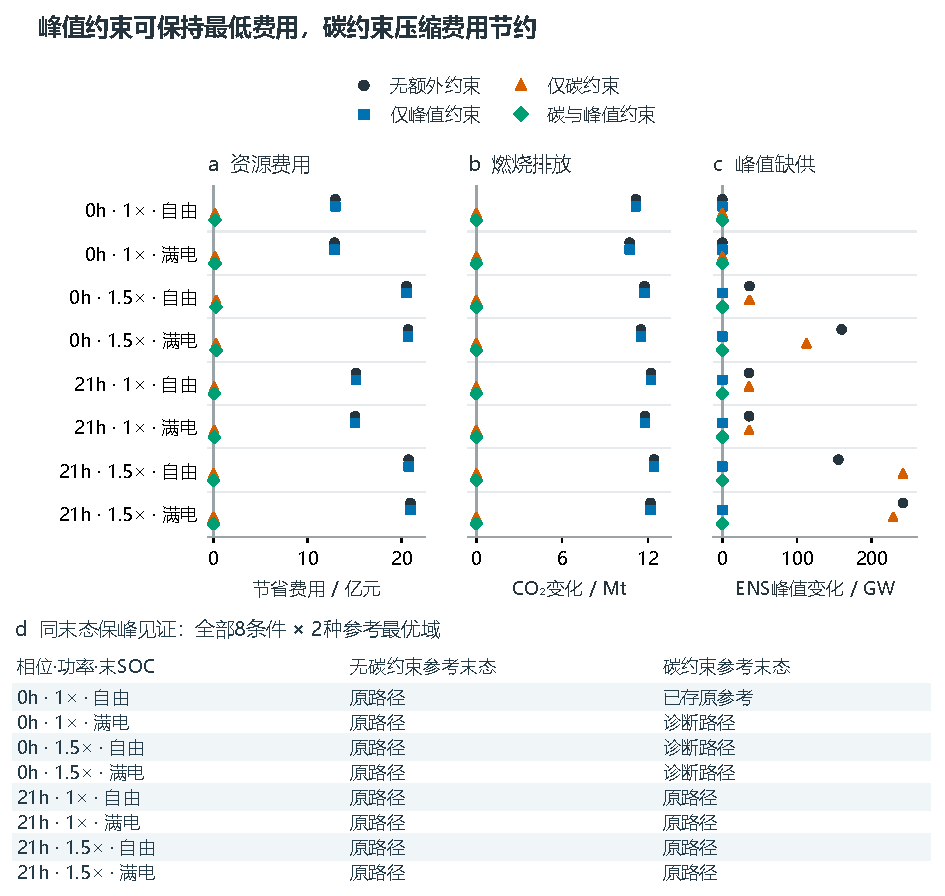
\includegraphics[width=160mm]{figures/figS_joint_dispatch_constraints.pdf}
\caption{同一缺供边界上的四类最优排程。a—c按全部八条件相对对应滚动路径比较费用、排放、峰值，主窗h48—359；实际前48小时固定，后312小时一次优化。ENS容差$10^{-6}$GWh，物理费含净SOC领用与持有费，不含碳价和缺供罚金。d保留全部16个同末态保峰见证，固定各自最优解的三燃料、两SOC与两热机末出力；“已存原参考”表示直接验证既有排程，$\le$10元不作收益。}\label{fig:joint-dispatch}\end{figure}

保峰是否占用了期末资源，还需在相同末态下比较。固定各自参考最优解的三种燃料库存、两项SOC及煤气末出力，16个条件均有费用数值等价的保峰排程；其中15个条件由新增成功解覆盖，另一个由原参考排程及其原域证书直接确认。完整尝试及求解器状态见附录，同末态比较的对象始终是各自参考解。

这一比较将操作目标落实为可检查的约束：累计能量边界由供给与可交付储能决定；同一边界内的小时缺口可重新分配；费用优化还必须同时查看排放与期末准备。资源费仍逐项核对燃料领用、非燃料运行、循环、移峰、净SOC领用和库存持有；各电源发电与费用分解、原最低费用图及全部末态列于附录。

\begin{table}[H]\centering\caption{关键工程参数的依据与作用}
\begin{tabularx}{\linewidth}{p{.18\linewidth}p{.25\linewidth}X}\toprule
参数 & 采用值 & 依据及在模型中的作用\\\midrule
储能配置 & 电池4小时，抽蓄6小时 & 工程配置；以官方2024多技术储能平均2.3小时增算单参数挑战\\
热机上爬坡 & 煤0.15、气0.70倍额定功率/小时 & 聚合工程约束，逐时限制由真实上期出力可达的本期出力\\
初始燃料储备 & 2024年按45天年消费初始化 & 年度初态设计；后续年度积累，小时层读取所选年份实际年末库存\\
联合恢复 & 服务缺失至多1\%，库存至少事件前95\%，持续24小时 & 本文操作判据；固定初始与同小时无事件库存另列参照\\
\bottomrule\end{tabularx}\end{table}
\FloatBarrier

\section{结论与应用建议}
多能源转型的安全性由建设兑现、运行交付与资源准备共同决定。三问形成可逐项核查的决策链。

现状上，2010—2024年一次能源消费增长65.3\%，化石服务与新能源扩张并行；主体模型通过独立料源、建设队列与交付约束承接这一矛盾。双碳推演中，基准至2060窗口末端仍未确认达峰，政策强化将2060剩余净排由12.639降至9.325 Gt；主体主动反馈的终点减排伴随跨期服务代价，评价需同时观察排放与交付。

投资上，折中路径比最低观察可靠资本多投入13.663万亿元、减少2060净排7.520 Gt，但原48组联合扰动仅3组年度可靠。保供修复将其增至20/48，另48组独立设计中21组达标，名义情景的折现资本增加26.526万亿元，2060年净排增加2.037 Gt。进口—工期网格定位不晚于2030年投产的油项目台阶；年度方案下钻小时层后，方案Ⅰ、方案Ⅲ在主窗满足电力交付，方案Ⅱ仍有8.827 TWh缺供。196条建设窗口对照中，窗口内扩建改善6组2030油缺口，却未提高20/48完整年度可靠数；全期扩大油气建设降至19/48。应先核对截止前实际可投产的队列，再配置国内建设与外部资源。

运行上，八组累计缺供均达到对应离线下界；原相位四段夜间守恒界为5.170 TWh。增加功率可改变小时缺口，改变累计电量还需可用供给、可交付储能或服务需求的变化。24臂联合约束进一步表明，八组最低费用均可同时守住原峰值；排放约束使降费空间从12.861—20.924亿元收缩为六组698.316—2738.648万元、两组数值等费。按累计能量、峰值、排放、费用与末态共同选择排程。

\begin{table}[H]\centering\caption{按瓶颈选择动作及其已检验作用}
\begin{tabularx}{\linewidth}{p{.15\linewidth}p{.23\linewidth}X}\toprule
识别的瓶颈 & 对应动作 & 完整路径中的实际作用\\\midrule
建设兑现与料源 & 分期资本及技术/供应订单 & 年度门槛、进口—工期网格与小时交付共同筛查所选组合\\
时序分配 & 联合协调储能、发电与偿还 & 对可达全电源余量局部规则，共同满电终点下原功率主窗少缺供109.455 GWh；32格中21格进一步改善\\
交付功率 & 功率增加50\%，能量固定 & 32格中29格削峰、5格减少累计缺供；原48小时设计削峰78.634 GW\\
跨事件准备 & 按时滞、渠道和资源目标补库 & 原付费合同增购末库存，新增现金、资产与溢价分账；四方案对原无事件目标的第二窗口库存仍低于95\%\\
\bottomrule\end{tabularx}\end{table}
三类运行动作分别对应时序、交付上限与资源补充。更强局部基线、事件信息、完整事件网格和2.3小时电池挑战给出收益的具体条件；库存以最近事件前、固定初始和同小时无事件三种参照共同解释。实际原生运行、完整跨实现路径与独立守恒账使方案、动作和结果衔接。工程应用时，以地区负荷、真实到货、库存和项目工期替换相应聚合输入，再按同一账本复验候选。

\subsection{五类协同对策与实施顺序}
\textbf{能源结构优化：先核投产窗口，再配置资本。}按截至目标年可兑现能力审查油气与电源订单。油工期为4、5、6年时，不晚于2030年投产的订单截止分别为2026、2025、2024年；窗口外的即时缺口应由已有队列、渠道及可用库存共同保障。P2改善6组单年油缺口而未提高全期可靠数，P3又出现新增电力失守，说明扩建须和其他资产交付共同评价。

\textbf{多能协同调度：同时检查能量、峰值与末态。}以实际状态滚动协调发电、储能和偿还，共同满电终点下相对强局部规则仍少缺供109.455 GWh。功率增加50\%在29/32格削峰、仅5格减少累计缺供；原相位已到四夜能量下界，应把功率配置与可交付能量分开决策，并直接加入峰值和排放约束选择费用排程。

\textbf{储备与应急建设：按到货时滞和资源目标补库。}把采购现金、末库存资产及溢价分别列账，本组1666.523亿元现金形成1111.016亿元资产和555.508亿元资源净增费。储备目标同时核对最近事件前、固定初始与同小时无事件库存；按跨境通道和合同到货条件落实资源，持续检查下一事件前的准备。

\textbf{市场机制设计：将稀缺与碳信号接到交付账。}联合评价价格规则诱发的订单、投产和需求变化。基准阶跃档位由800升至1200元/MWh时，2060年能源CO$_2$少0.200 Gt，累计未供服务却由19.608增至35.427 PWh；同档平滑规则为20.687 PWh。设计价格与碳反馈时，应同步比较供能、工程资本及资源费用，避免以终点减排替代完整服务评价。

\textbf{科技创新：以能量和工业净排缺口确定研发方向。}同一功率下，电池由4小时缩至2.3小时使原事件累计缺供增加396.654 GWh，可交付电量是独立的配置对象。基准工业过程与固定碳汇假设下仍有175.346 Mt结构净排下界，需要将工业深度减排或新增移除作为后续技术选项单独评价，不能只靠现有发电结构调整兑现净零。

实施上，近期先使用现有运行数据重排调度、明确库存目标和有效订单窗口；中期落实渠道、合同与已批准建设队列；长期依据地区负荷、到货和技术成本评价新增能量容量及工业减排。每一步均以实际交付、完整资源账和资本代价复核。


\begin{table}[!htbp]\centering\caption{模型口径与检验层次}\label{tab:scope}
\begin{tabularx}{\linewidth}{p{.15\linewidth}XX}\toprule
对象 & 实现与依据 & 结果的统一解释\\\midrule
历史分类 & 年鉴“一次电力及其他能源”保持原分类；前瞻以七类电源构造非化石工程映射 & 历史第四分类与模型非化石结果分别命名，分类映射用于条件比较\\
工程与行为 & 全国聚合母线、连续机组、外生水电可用率；建设、退役、成本及响应部分校准 & 217维为状态维数；12类资产承担投资选择，小时出力按聚合母线与连续爬坡执行\\
进口折标 & 煤、原油和天然气用官方参考系数，成品油以燃料油系数作聚合代表 & 基年满足$rP+I=C$；平衡调节项单列，折标低档在物理域内修订为$-2\%$\\
历史检验 & 固定起点、给定已实现GDP的共享预期与资产组件检验 & 用于组件误差诊断；独立进口映射从2024年前瞻起点生效\\
机制比较 & 主实验保留自主趋势、关闭主动响应；冻结份额另作诊断 & 主动反馈贡献与外生载能趋势分开解释；较高近期需求外推只作需求压力对照\\
尺度与信息 & 年度内部闭环，关键年状态单向下钻；原生试验24小时前瞻，信息挑战只改变事件可见时长 & 滚动控制采用24小时优化窗；离线参照固定实际前48小时后一次优化312小时；年度投资仍由年度规则产生\\
事件与恢复 & 工程天气、负荷和到货；连续继承燃料、SOC、爬坡记忆和债务 & 对应固定设计事件集合；库存以事件前、固定初始及同小时无事件分别参照，格点数描述工程条件覆盖\\
费用与搜索 & 按模拟订单付资；工程资本、小时资源费用、合同现金分账；固定预算搜索 & 固定方案保留开发48组与另48组独立设计；新建设机制在原开发48组内配对比较\\
碳核算 & 年度历史有效映射加简化工业与固定碳汇；小时用IPCC燃烧系数 & 年度剩余净排衡量所选技术组合下的中和缺口；小时报告实际燃料燃烧CO$_2$\\
\bottomrule\end{tabularx}\end{table}\FloatBarrier

\FloatBarrier\clearpage
\begingroup\small
\begin{thebibliography}{99}\setlength{\itemsep}{2pt}\addcontentsline{toc}{section}{参考文献}
\bibitem{contest} 赛事组委会. 2026年第二届全国大学生仿真建模应用挑战赛A题：双碳背景下多种能源融合发展系统仿真与优化研究[竞赛题面与评分表]. 2026.
\bibitem{nbs_yearbook_2025_9_2} 中国统计年鉴2025 表9-2 能源消费总量及构成[EB/OL]. 保存版访问日期：2026-10-16. \url{https://www.stats.gov.cn/sj/ndsj/2025/html/C09-02.jpg}.
\bibitem{nbs_yearbook_2025_9_1} 中国统计年鉴2025 表9-1 一次能源生产总量及构成[EB/OL]. 保存版访问日期：2026-10-16. \url{https://www.stats.gov.cn/sj/ndsj/2025/html/C09-01.jpg}.
\bibitem{ember_latest_2026_10_16} Ember Yearly Electricity Data, current global release[EB/OL]. 保存版访问日期：2026-10-16. \url{https://files.ember-energy.org/public-downloads/generation/outputs/release_generation_yearly_global.csv}.
\bibitem{worldbank_NY.GDP.MKTP.KD} World Bank World Development Indicators GDP constant 2015 US\$[EB/OL]. 保存版访问日期：2026-10-16. \url{https://api.worldbank.org/v2/country/CHN/indicator/NY.GDP.MKTP.KD?format=json&date=2010:2025&per_page=100}.
\bibitem{owid_gcb_2025} OWID CO2 dataset based on Global Carbon Budget 2025[EB/OL]. 保存版访问日期：2026-10-16. \url{https://raw.githubusercontent.com/owid/co2-data/master/owid-co2-data.csv}.
\bibitem{nea_electricity_2024} 国家能源局 2024年全社会用电量同比增长6.8\%[EB/OL]. 保存版访问日期：2026-10-16. \url{https://www.nea.gov.cn/20250120/4f7f249bac714e7693adecac996d742f/c.html}.
\bibitem{nbs_energy_method} 中国统计年鉴2025 能源篇简要说明[EB/OL]. 保存版访问日期：2026-10-16. \url{https://www.stats.gov.cn/sj/ndsj/2025/html/sm09.htm}.
\bibitem{nbs_energy_faq} 七、能源统计（21）[EB/OL]. 保存版访问日期：2026-10-16. \url{https://www.stats.gov.cn/hd/cjwtjd/202302/t20230207_1902276.html}.
\bibitem{nbs_communique_2024} 国家统计局. 中华人民共和国2024年国民经济和社会发展统计公报，表12主要商品进口数量[EB/OL]. 2025-02-28，访问日期2026-10-18. \url{https://www.stats.gov.cn/zwfwck/sjfb/202502/t20250228_1958817.html}.
\bibitem{nea_gas_development_2025} 国家能源局石油天然气司等. 中国天然气发展报告（2025）[R/OL]. 2025，印刷页7，访问日期2026-10-18. \url{https://www.nea.gov.cn/20250829/a4e2deb9b6444df1a191b9d60c111ffd/20250829a4e2deb9b6444df1a191b9d60c111ffd_43ab87a785d1b64d49b9210dbc15d3781e.pdf}.
\bibitem{nbs_yearbook_2025_9_19} 中国统计年鉴2025 表9-19 分地区主要能源产品产量[EB/OL]. 保存版访问日期：2026-10-16. \url{https://www.stats.gov.cn/sj/ndsj/2025/html/C09-19.jpg}.
\bibitem{nbs_prices_2024_dec_late} 2024年12月下旬流通领域重要生产资料市场价格变动情况[EB/OL]. 保存版访问日期：2026-10-16. \url{https://www.stats.gov.cn/xxgk/sjfb/zxfb2020/202501/t20250103_1958140.html}.
\bibitem{nea_renewable_2024} 国家能源局 2024年可再生能源并网运行情况[EB/OL]. 保存版访问日期：2026-10-16. \url{https://www.nea.gov.cn/20250221/e10f363cabe3458aaf78ba4558970054/c.html}.
\bibitem{nea_hydrogen_2025} 中国氢能发展报告（2025）[EB/OL]. 保存版访问日期：2026-10-16. \url{https://www.nea.gov.cn/20250430/96022785b3a747248288ad1c57d3a025/83d863317f2f44edb605348e4de40993.pdf}.
\bibitem{ndrc_conversion} 国家发展改革委等. 合成纤维制造业（维纶）清洁生产评价指标体系[EB/OL]. 2019，附录C：各种能源折标准煤系数，访问日期2026-10-18. \url{https://www.ndrc.gov.cn/xxgk/zcfb/gg/201901/W020190905485836987613.pdf}.
\bibitem{nbs_conversion} 国家统计局. 第二次全国经济普查方案：能源统计表及主要能源折标准煤参考系数[EB/OL]. 保存版访问日期2026-10-18. \url{https://www.stats.gov.cn/zt_18555/zdtjgz/zgjjpc/decqgjjpc_19354/pcfa2/202303/t20230306_1929620.html}.
\bibitem{mathworks_linprog} MathWorks. linprog: Solve linear programming problems[EB/OL]. \url{https://www.mathworks.com/help/optim/ug/linprog.html}.
\bibitem{ipcc} IPCC. 2006 IPCC Guidelines for National Greenhouse Gas Inventories, Volume 2: Energy, Chapter 2, Table 2.2[EB/OL]. \url{https://www.ipcc-nggip.iges.or.jp/public/2006gl/pdf/2_Volume2/V2_2_Ch2_Stationary_Combustion.pdf}.
\bibitem{mathworks_step} MathWorks. Simulation.step: Advance simulation by a specified number of steps[EB/OL]. \url{https://www.mathworks.com/help/simulink/slref/simulink.simulation.step.html}.
\bibitem{anymath_docs} AnyMath文档. 软件控制建模[EB/OL]. 访问日期2026-10-18. \url{https://engee.com/helpcenter/stable/cn/modeling/programmatic-modeling.html}.
\bibitem{ai_tool} OpenAI Codex，GPT-6系列（具体服务版本以平台记录为准），OpenAI，2026年10月16—20日。
\bibitem{submission} 模竞平台. 2026年参赛须知[EB/OL]. 2026-10-10. \url{https://www.mojinghub.com/news/137}. 源程序须同时列入论文附录和支撑材料；提交细节以赛事最终官方通知为准.
\bibitem{nea_storage_2025} 国家能源局能源节约和科技装备司，电力规划设计总院. 中国新型储能发展报告（2025）[R/OL]. 2025，印刷页11，PDF第21页，访问日期2026-10-19. \url{https://www.nea.gov.cn/20250731/1d40d09f75714280a9218d5bea178fbd/228ab8631dcc4b2293c84dc1f07e6e42.pdf}.
\bibitem{nrel_atb_storage} NREL. 2024 Annual Technology Baseline: Utility-Scale Battery Storage[EB/OL]. 2024，访问日期2026-10-19. \url{https://atb.nlr.gov/electricity/2024/utility-scale_battery_storage}.
\bibitem{scipy_highs_1153} SciPy. linprog HiGHS、dual simplex与interior point接口，版本1.15.3[EB/OL]. 访问日期2026-10-19. \url{https://docs.scipy.org/doc/scipy-1.15.3/reference/optimize.linprog-highs.html}; \url{https://docs.scipy.org/doc/scipy-1.15.3/reference/optimize.linprog-highs-ds.html}; \url{https://docs.scipy.org/doc/scipy-1.15.3/reference/optimize.linprog-highs-ipm.html}.
\bibitem{official_station_lists}赛事组委会. A题附件1—4：火电、水电、抽蓄、风电和核电站名录[DS]. 2026年随题Excel原件；参考年份与抽样设计未声明。原件及逐表核查见支撑材料\path{data/v17/official_attachments/}与\path{outputs/v17/stations/}.
\end{thebibliography}
\endgroup

\subsection*{辅助工作说明}
本作品由参赛团队统筹并对提交内容负责。OpenAI Codex（GPT-6系列，OpenAI；2026年10月16—20日）作为辅助工具，用于资料检索整理、模型实现与校核、程序调试、图表绘制排版及文字修改\cite{ai_tool}。相关模型、参数与结论以正文、原始资料及实际计算结果为依据。
\label{body-end}\clearpage

\appendix
\section{支撑材料与程序索引}\label{appendix-start}
\subsection{目录与复现入口}
支撑材料包含本版论文对应的模型、原始资料、参数配置、保存的计算结果、图表生成代码及本稿源文件。源文件沿用实际调用所需的名称；目录中的编号用于标识计算核与结果来源。
\begin{table}[H]\centering\caption{本版支撑材料目录与入口}
\begin{tabularx}{\linewidth}{p{.20\linewidth}X}\toprule
目录或入口 & 内容与用途\\\midrule
\path{src/} & 年度模型、投资搜索、连续事件、约束核验和图文生成程序\\
\path{config/} & 模型参数、情景与固定实验配置\\
\path{data/} & 官方附件、原始资料与预处理数据\\
\path{simulation/} & MATLAB/Simulink与AnyMath原生模型、控制器和状态接口\\
\path{outputs/} & 本文计算结果、逐案状态、矩阵、配对表和求解记录\\
\path{figures/} & 当前图件的可编辑矢量文件\\
\path{paper/} & 本版论文TeX稿源与正文使用图件\\
\bottomrule\end{tabularx}\end{table}
\noindent\textbf{图表与论文：}\texttt{复现图表与论文.py}，读取随附结果、重绘图表并编译论文。\par
\noindent\textbf{MATLAB：}\path{start_v9_lab.m}，启动原生物理网络与交互实验台。\par
\noindent\textbf{AnyMath：}\path{simulation/anymath_v10/start_v10.jl}，启动原生小时滚动优化。\par

\subsection{原生状态连接与计算入口}\label{app:anymath-native}
MATLAB原生环境采用R2026a、Simulink及Optimization Toolbox，小时求解调用\texttt{linprog}。实验台聚焦折中2060快照：控制器提出动作，原生物理网络推进库存、SOC、债务和机组记忆；支持初始化、单步、24小时推进、连续与暂停。回放读取已执行完整轨迹并单独标识；改变原生输入后重新初始化。

\begin{figure}[H]\centering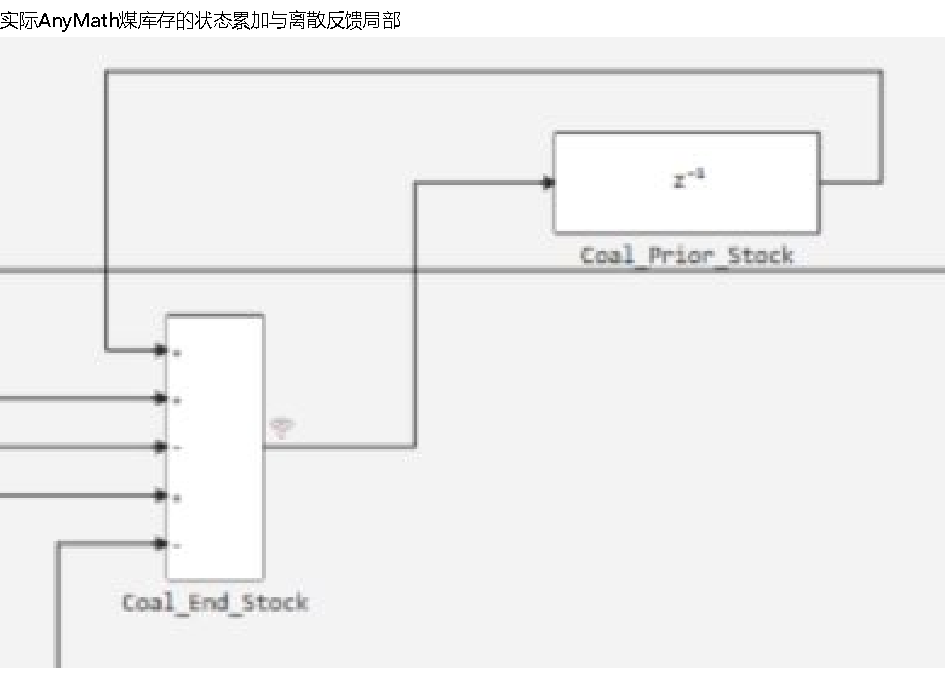
\includegraphics[width=\linewidth]{figures/native_anymath_state_feedback.pdf}\caption{实际平台截图的状态反馈局部。左侧信号进入Coal\_End\_Stock加和模块，更新库存经Coal\_Prior\_Stock离散延迟反馈到下一步。}\end{figure}

Python执行年度实验、可靠性投资搜索与连续事件计算，图表读取保存结果。年度与历史检验的对应程序为\path{src/v6_annual_experiments.py}，投资搜索程序为\path{src/v6_planning.py}，连续事件程序为\path{src/v6_resilience.py}。离线边界与守恒证据对应\path{src/v15_dispatch_bound_v2.py}和\path{src/v15_energy_cut_certificate.py}；联合约束、末态与数值表示核验对应\path{src/v16_joint_dispatch.py}、\path{src/v16_endpoint_peak.py}、\path{src/v16_endpoint_numerics.py}和\path{src/v16_endpoint_bound_form.py}。原始求解状态与失败记录和成功结果一并保留。

AnyMath每小时以上一实际末状态初始化原生记忆，在\texttt{StopTime=0}处求值一个隐含$\Delta t=1$ h的离散资源转移，返回8维末状态后继续优化；小时索引由外层会话推进。滚动LP存在多最优解，跨实现核验比较同状态最优目标与物理可行性，不要求首动作唯一。实际云执行含中断后从同版本、同8维末状态续算的路径，前缀与衔接核对保留在对应计算结果中。

\section{原生原型与最优解选择的补充图表}
\subsection{储能状态如何改变高峰时的实际交付}
实验台显示当前方案、供给方式、策略及实际已执行小时。原生模式支持初始化、单步、24小时推进、连续和暂停，曲线仅显示已求解前缀；保存轨迹回放使用独立标识。输入改变后重新初始化，避免把新参数套在旧状态上。
\begin{figure}[H]\centering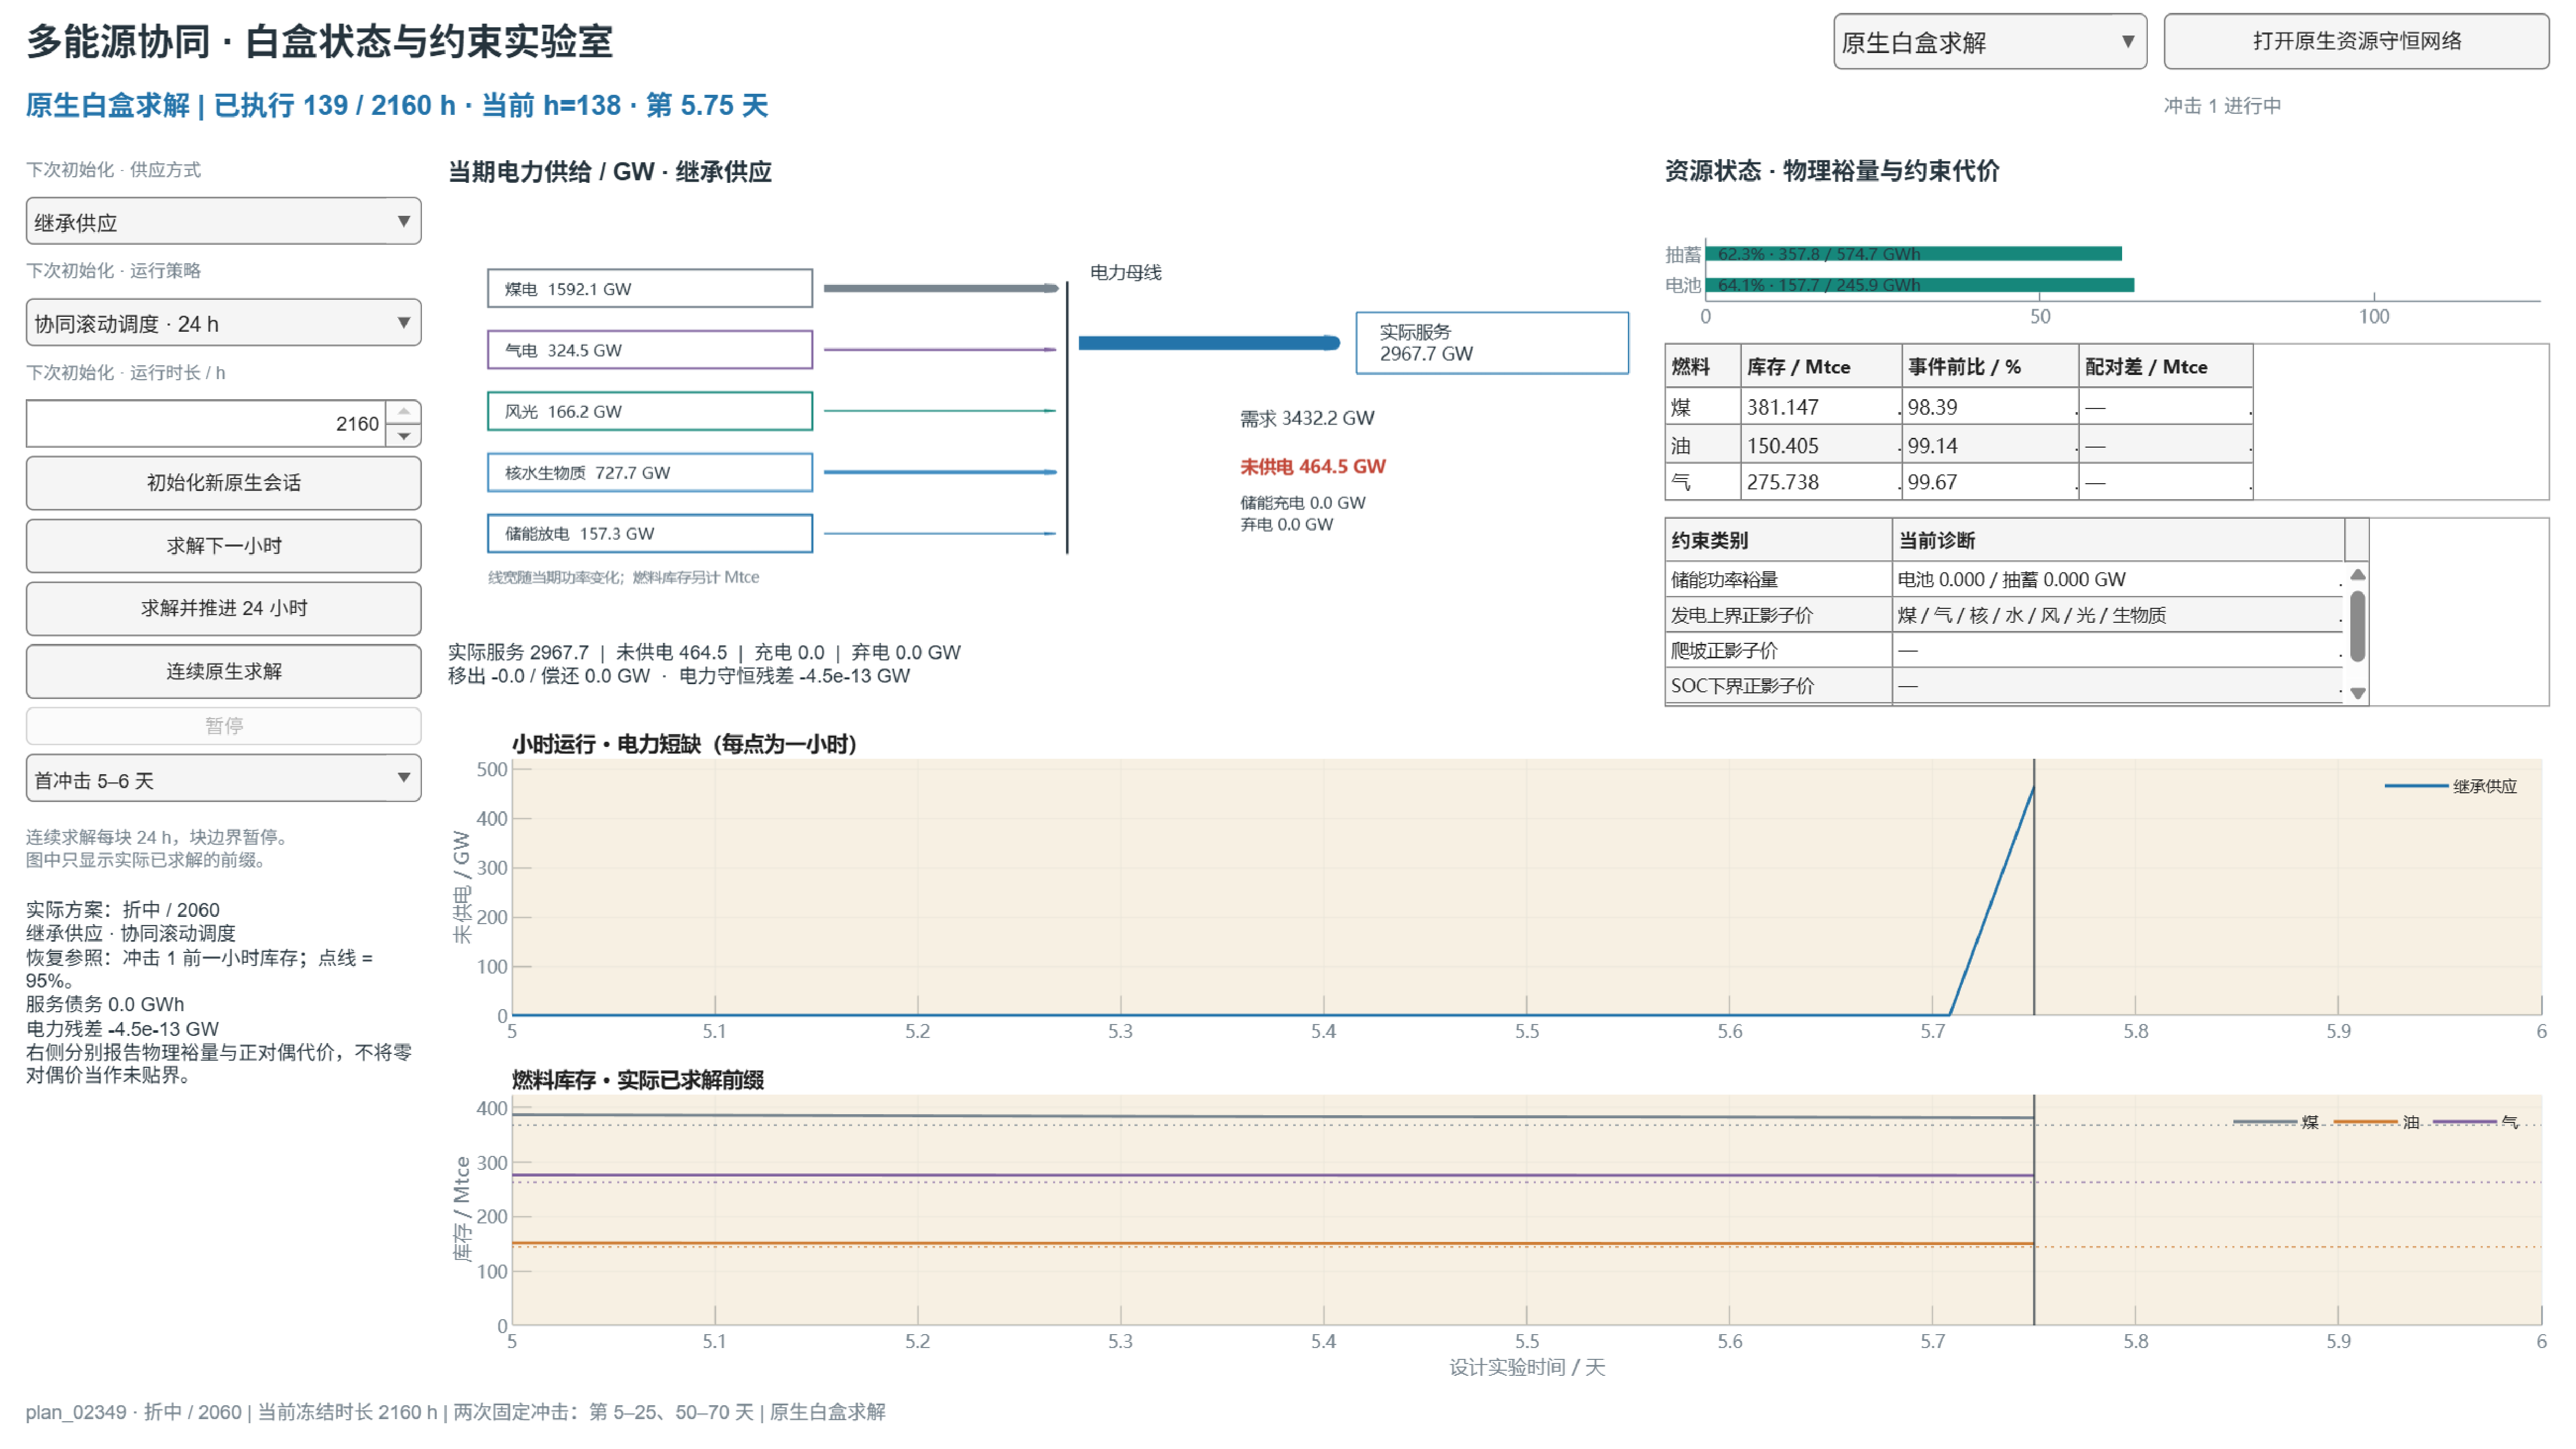
\includegraphics[width=160mm]{figures/native_v9_app_overview.pdf}\caption{实际原生求解至h=138的过程实验台。能流与库存对应同一小时，窗口同时显示已执行前缀、缺供和约束状态；该截图来自新物理资源网络。}\end{figure}

\begin{table}[H]\centering\caption{相同初态与外部输入下的两条原生状态路径}
\begin{tabular}{lrr}\toprule
状态或交付 & 协调 & 分散\\\midrule
h=137末电池SOC / GWh & 222.478 & 0.000 \\
h=137末抽蓄SOC / GWh & 466.240 & 0.000 \\
h=138电池放电 / GW & 61.487 & 0.000 \\
h=138抽蓄放电 / GW & 95.782 & 0.000 \\
h=138未供电 / GW & 464.457 & 621.726 \\
h=0--144累计未供电 / GWh & 1,530.829 & 2,271.709 \\
\bottomrule\end{tabular}\end{table}

第137小时末，协调路径仍保留电池与抽蓄能量，分散路径已耗尽。第138小时，两类储能合计交付157.269 GW，恰与两路径该小时的缺电差对应；截至第144小时，协调路径累计少缺供740.879 GWh。

将两种策略从\textbf{同一个第137小时末状态、同一未来24小时输入}重新分支，第138小时未供电均为464.457 GW，差值为零。因此，这一峰时的路径收益来自此前形成的储能状态，而非同状态下该时刻产生了更高的即时供电。此处聚焦协调与分散各145小时的状态路径；前述90天交付与库存结果，另由两种供应方式下各2160小时的完整原生运行核对。
\FloatBarrier


\begin{figure}[H]\centering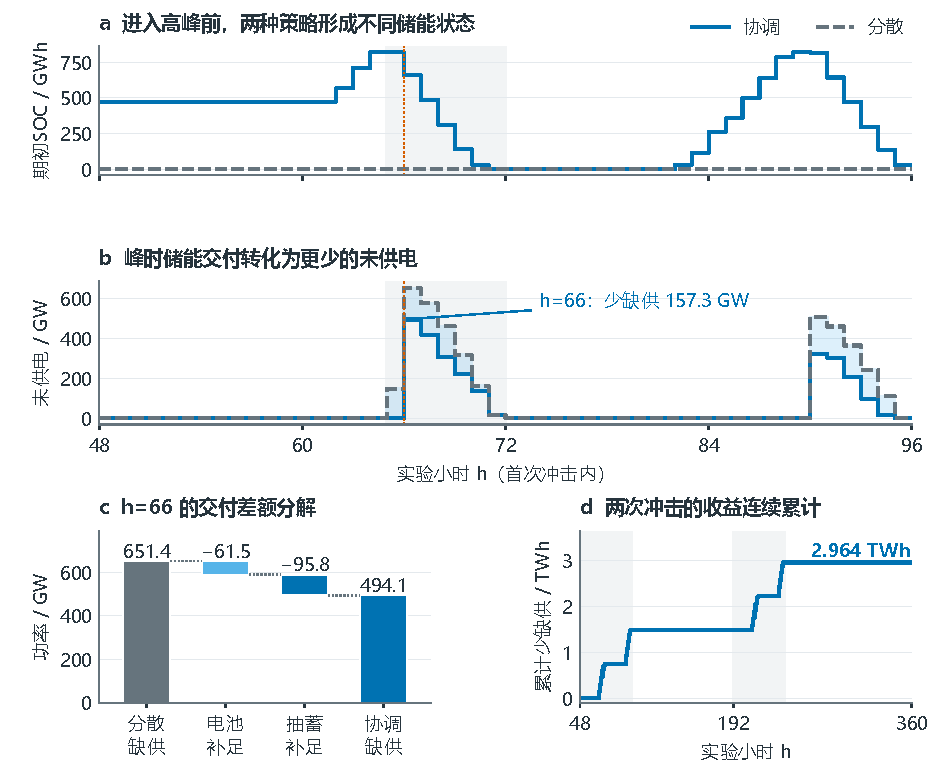
\includegraphics[width=\linewidth]{figures/figH_coordination_mechanism.pdf}
\caption{协调相对指定非化石局部规则的动作链：首次冲击内的逐小时期初SOC、峰值时储能交付及累计缺供。各面板读取相同已执行轨迹，收益统计统一为第48—359小时。}\label{fig:figH_coordination_mechanism}\end{figure}

\begin{figure}[H]\centering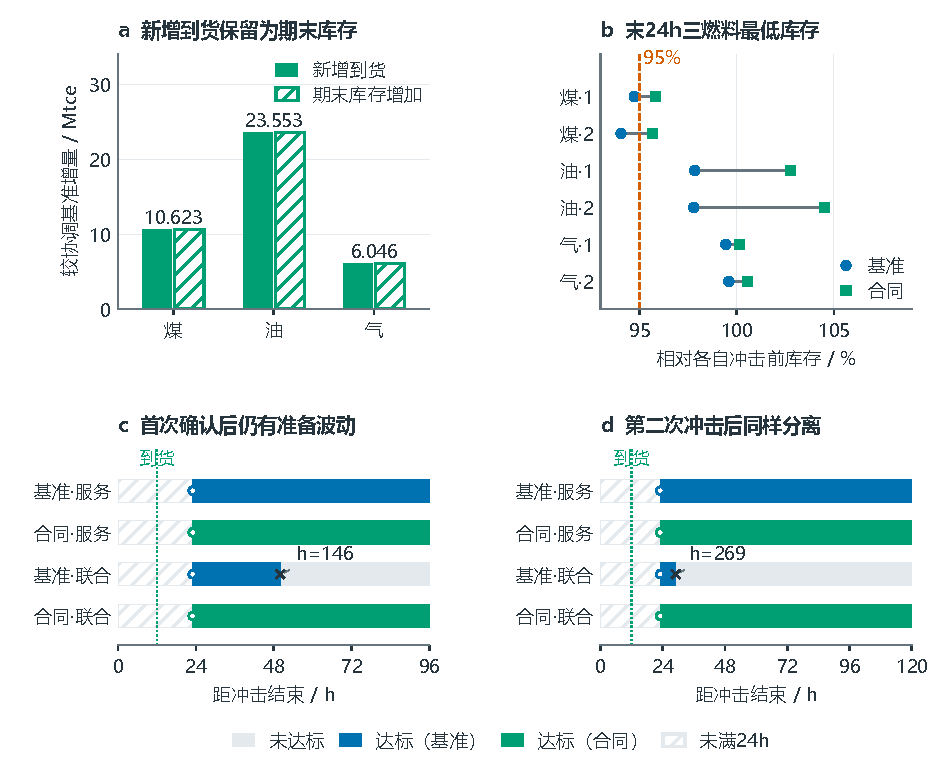
\includegraphics[width=\linewidth]{figures/figJ_contract_readiness.pdf}
\caption{合同到货如何形成资源准备。新增到货与末库存增量逐燃料核对；库存底线取事件边界前完整24小时内的最小比值，分母为各方案各事件的冲击前库存。色带分别表示服务窗口与联合准备窗口。}\label{fig:figJ_contract_readiness}\end{figure}

\begin{figure}[H]\centering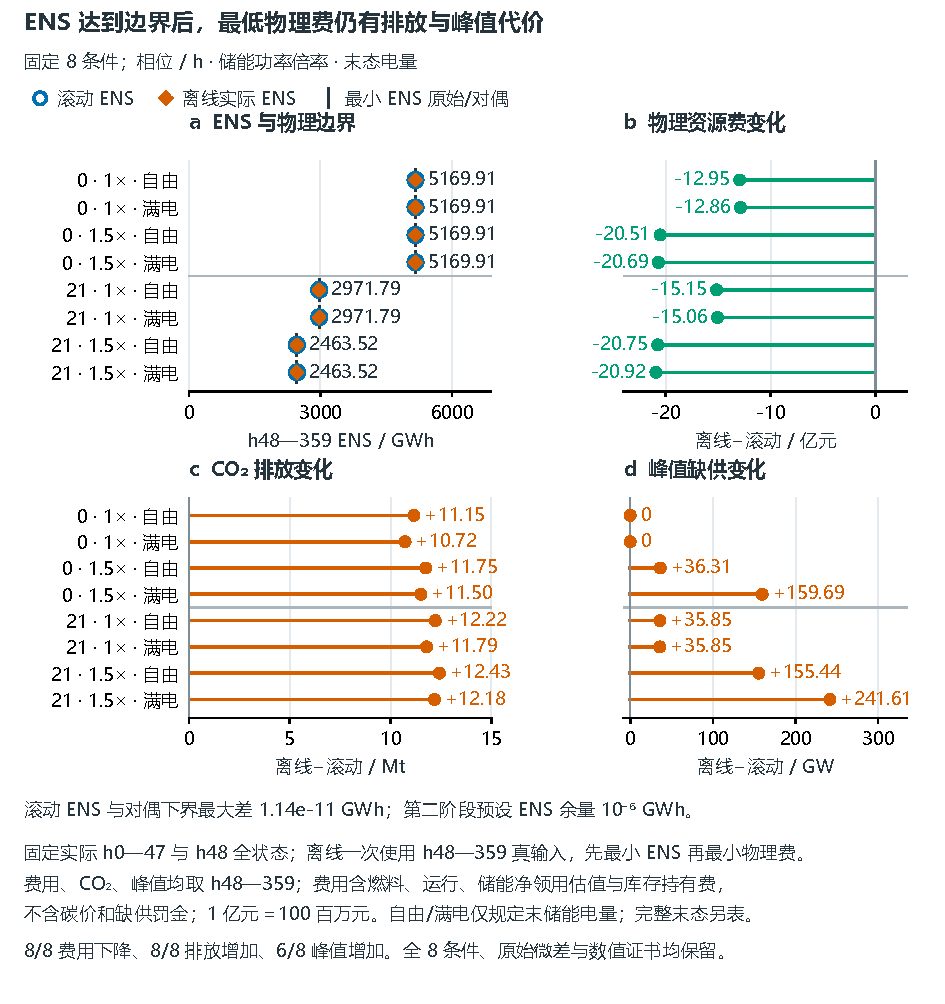
\includegraphics[width=160mm]{figures/figQ_dispatch_bound_tradeoffs.pdf}
\caption{固定前缀下的八组离线参照：累计缺供边界、物理资源费、排放及峰值。二阶段允许$10^{-6}$ GWh缺供容差；此图保留当次求解器选出的最优解；六条峰值升高均另有等费保峰替代，见正文联合约束图。原值与完整末态见配对表。}\end{figure}

\begin{table}[H]\centering\caption{原相位四个夜间窗口的守恒电量下界}
\begin{tabular}{rrrr}\toprule
全局小时h & \shortstack{可用发电后缺口\\GWh} & \shortstack{储能最大交付\\GWh} & \shortstack{ENS下界\\GWh}\\\midrule
65—71 & 2328.016 & 740.879 & 1587.137 \\
89—95 & 1680.148 & 740.879 & 939.268 \\
209—215 & 2306.845 & 740.879 & 1565.966 \\
233—239 & 1818.419 & 740.879 & 1077.539 \\
\bottomrule\end{tabular}
\smallskip\par\noindent 各窗结束于原24小时债务截止点；按七种电源可用出力计算，各储能允许从满电开始。
\end{table}\section{联合约束、数值表示与完整状态记录}
联合约束24案完整成功。附加同末态原16案保留12成功与4个求解器状态2；关闭预处理的8次诊断保留2成功与6个状态2。末态等式改写为同值固定界的最后8次另列独立身份，全部实际状态见完整状态表；成功解同时核对原矩阵KKT与360小时物理转移。算法诊断不计为独立工程条件。两法按SciPy 1.15.3官方接口设置，实际选项与环境保存在冻结协议中\cite{scipy_highs_1153}。

\begin{table}[H]\centering\caption{同末态固定队列的完整原始求解状态}
\begin{tabular}{llccccc}\toprule
\shortstack{相位/功率/\\末SOC} & 参考 & 原表示 & DS & IPM & \shortstack{等价\\DS} & \shortstack{等价\\IPM}\\\midrule
0/1/自由 & 无碳帽 & 成功 & — & — & — & — \\
0/1/自由 & 碳封顶 & 状态2 & 状态2 & 状态2 & 状态2 & 状态2 \\
0/1/满电 & 无碳帽 & 成功 & — & — & — & — \\
0/1/满电 & 碳封顶 & 状态2 & 成功 & 状态2 & 状态2 & 状态2 \\
0/1.5/自由 & 无碳帽 & 成功 & — & — & — & — \\
0/1.5/自由 & 碳封顶 & 状态2 & 状态2 & 成功 & 成功 & 状态2 \\
0/1.5/满电 & 无碳帽 & 成功 & — & — & — & — \\
0/1.5/满电 & 碳封顶 & 状态2 & 状态2 & 状态2 & 状态2 & 成功 \\
21/1/自由 & 无碳帽 & 成功 & — & — & — & — \\
21/1/自由 & 碳封顶 & 成功 & — & — & — & — \\
21/1/满电 & 无碳帽 & 成功 & — & — & — & — \\
21/1/满电 & 碳封顶 & 成功 & — & — & — & — \\
21/1.5/自由 & 无碳帽 & 成功 & — & — & — & — \\
21/1.5/自由 & 碳封顶 & 成功 & — & — & — & — \\
21/1.5/满电 & 无碳帽 & 成功 & — & — & — & — \\
21/1.5/满电 & 碳封顶 & 成功 & — & — & — & — \\
\bottomrule\end{tabular}
\smallskip\par\noindent DS为双单纯形，IPM为内点法；两轮诊断均关闭预处理。破折号表示该条件未列入该轮固定四案，不是求解失败。状态2保留求解器原返回值，不能单独作为物理不可行证明。算法不计为独立工程条件。
\end{table}
\begin{table}[H]\centering\caption{四个原参考向量的完整零求解见证检查}
\begin{tabular}{llr}\toprule
相位/功率/末SOC & 原域见证 & 峰值减上界/GW\\\midrule
0/1/自由 & 有效 & 0.000000 \\
0/1/满电 & 有效 & 0.000000 \\
0/1.5/自由 & 峰值超界 & 36.314724 \\
0/1.5/满电 & 峰值超界 & 112.849882 \\
\bottomrule\end{tabular}
\smallskip\par\noindent 四个参考全部检查，保留两个超界负项。原功率自由/满SOC参考通过原域KKT与既有360小时物理来源核对；其中自由案补齐最后一种见证。原参考全部沿用已保存轨迹，新增LP与新增物理小时均为零。
\end{table}
固定末库存还揭示约束结构。对同一到货与直接服务路径，燃料总领用$Q_f=S_{f,48}+\sum I_{f,t}-S_{f,360}$，因此$C=\sum_f\epsilon_fQ_f$随三燃料末库存确定。独立代数核查将936条燃料余额等式按原排放系数加权并扣除三条末库存等式，所得系数与碳上界行的最大差为$1.09\times10^{-19}$，RHS差为$6.54$—$7.56\times10^{-12}$ Mt。该冗余与两方法分歧一并保留，不以单次状态2判定物理域为空。

\noindent 关键逐行结果见\path{outputs/v16/joint_dispatch_figures/}；八组工程条件、原16案和两轮诊断的全部失败均保留。\par

\section{结果标识与精确参数}
方案Ⅰ、Ⅱ、Ⅲ分别对应程序标识005、006、007。第21号联合设计的GDP增速倍率为1.186736，资本倍率为0.782592，进口倍率为0.760028。全部建设机制差值以图中明确的P0参照报告，原48组、32事件格与全部八组约束比较的原值均保留在支撑材料。表内舍入值用于阅读，精确值以对应原始计算表为准。

官方附件处理入口为\path{src/v17_station_evidence.py}，本版图件入口为\path{src/v18_main_visuals.py}和\path{src/v18_evidence_visuals.py}；论文稿源位于\texttt{paper/V18成果稿/}。

\end{document}
